



%----------------------------------------------------------------------------------------

\newpage

%%%%%%%%%%%%%%%%%%%%%%%
\section{Static Correlations}{Correlations Statiques}

\label{app:sec:staticcorrelations}



%%%%%%%%%%%%%%%%%%%%%%%
\subsection{Morphological Measures}{Mesures morphologiques}


% No need fo distributions, maps enough.
%%%%%%%%%%%%%%%%%%%
%\begin{figure}
%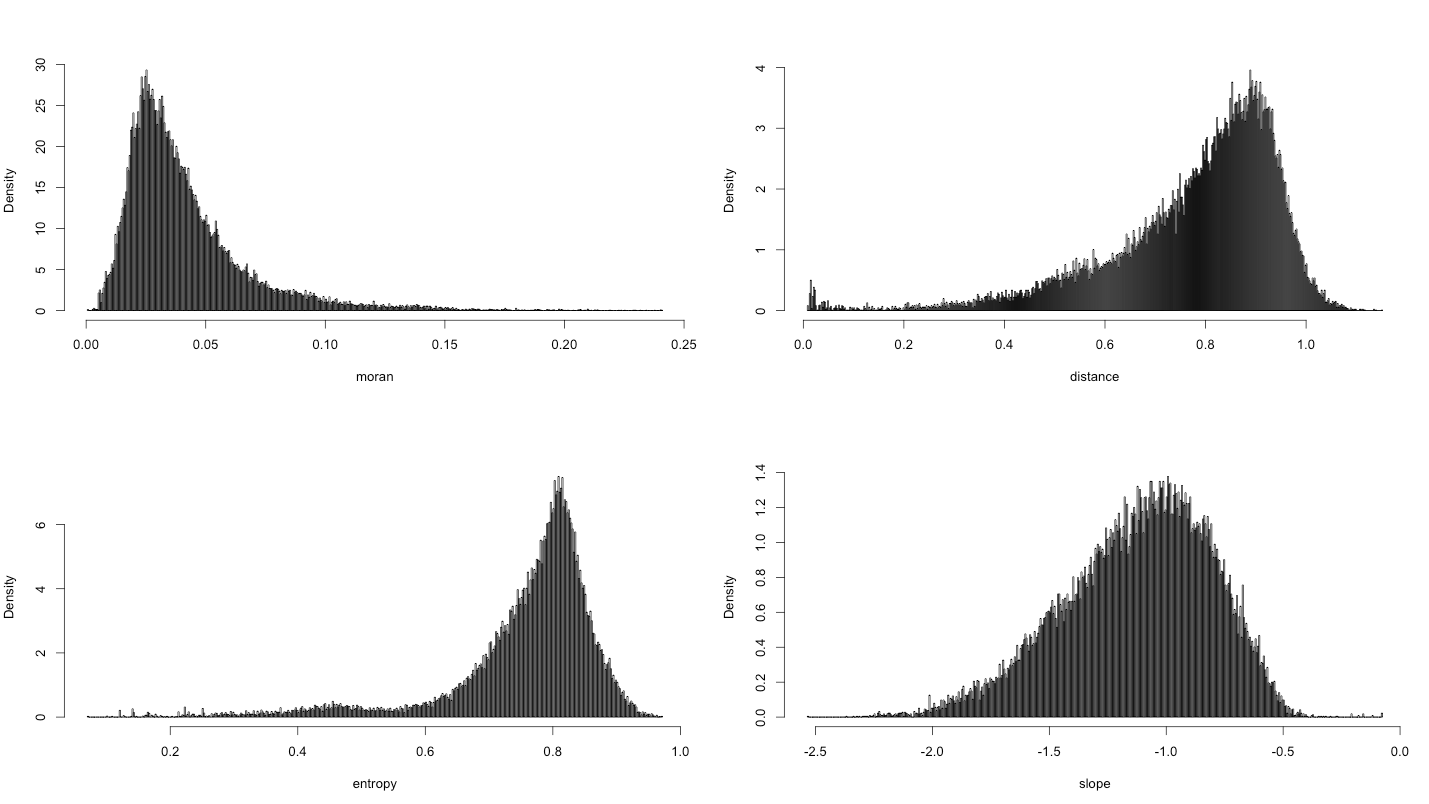
\includegraphics[width=1.2\textwidth]{Figures/Static/Density/hists_GOOD}
%\caption[Empirical Distribution of Morphological Indicators]{Empirical Distribution of Morphological Indicators}{Distribution empirique des indicateurs morphologiques\comment{(Florent) titres/labels illisibles ; dans quelle perspective as tu calculé ces indicateurs/affiché l'histogramme ?}}
%\end{figure}
%%%%%%%%%%%%%%%%%%
%




%%%%%%%%%%%%%%
\begin{figure}
%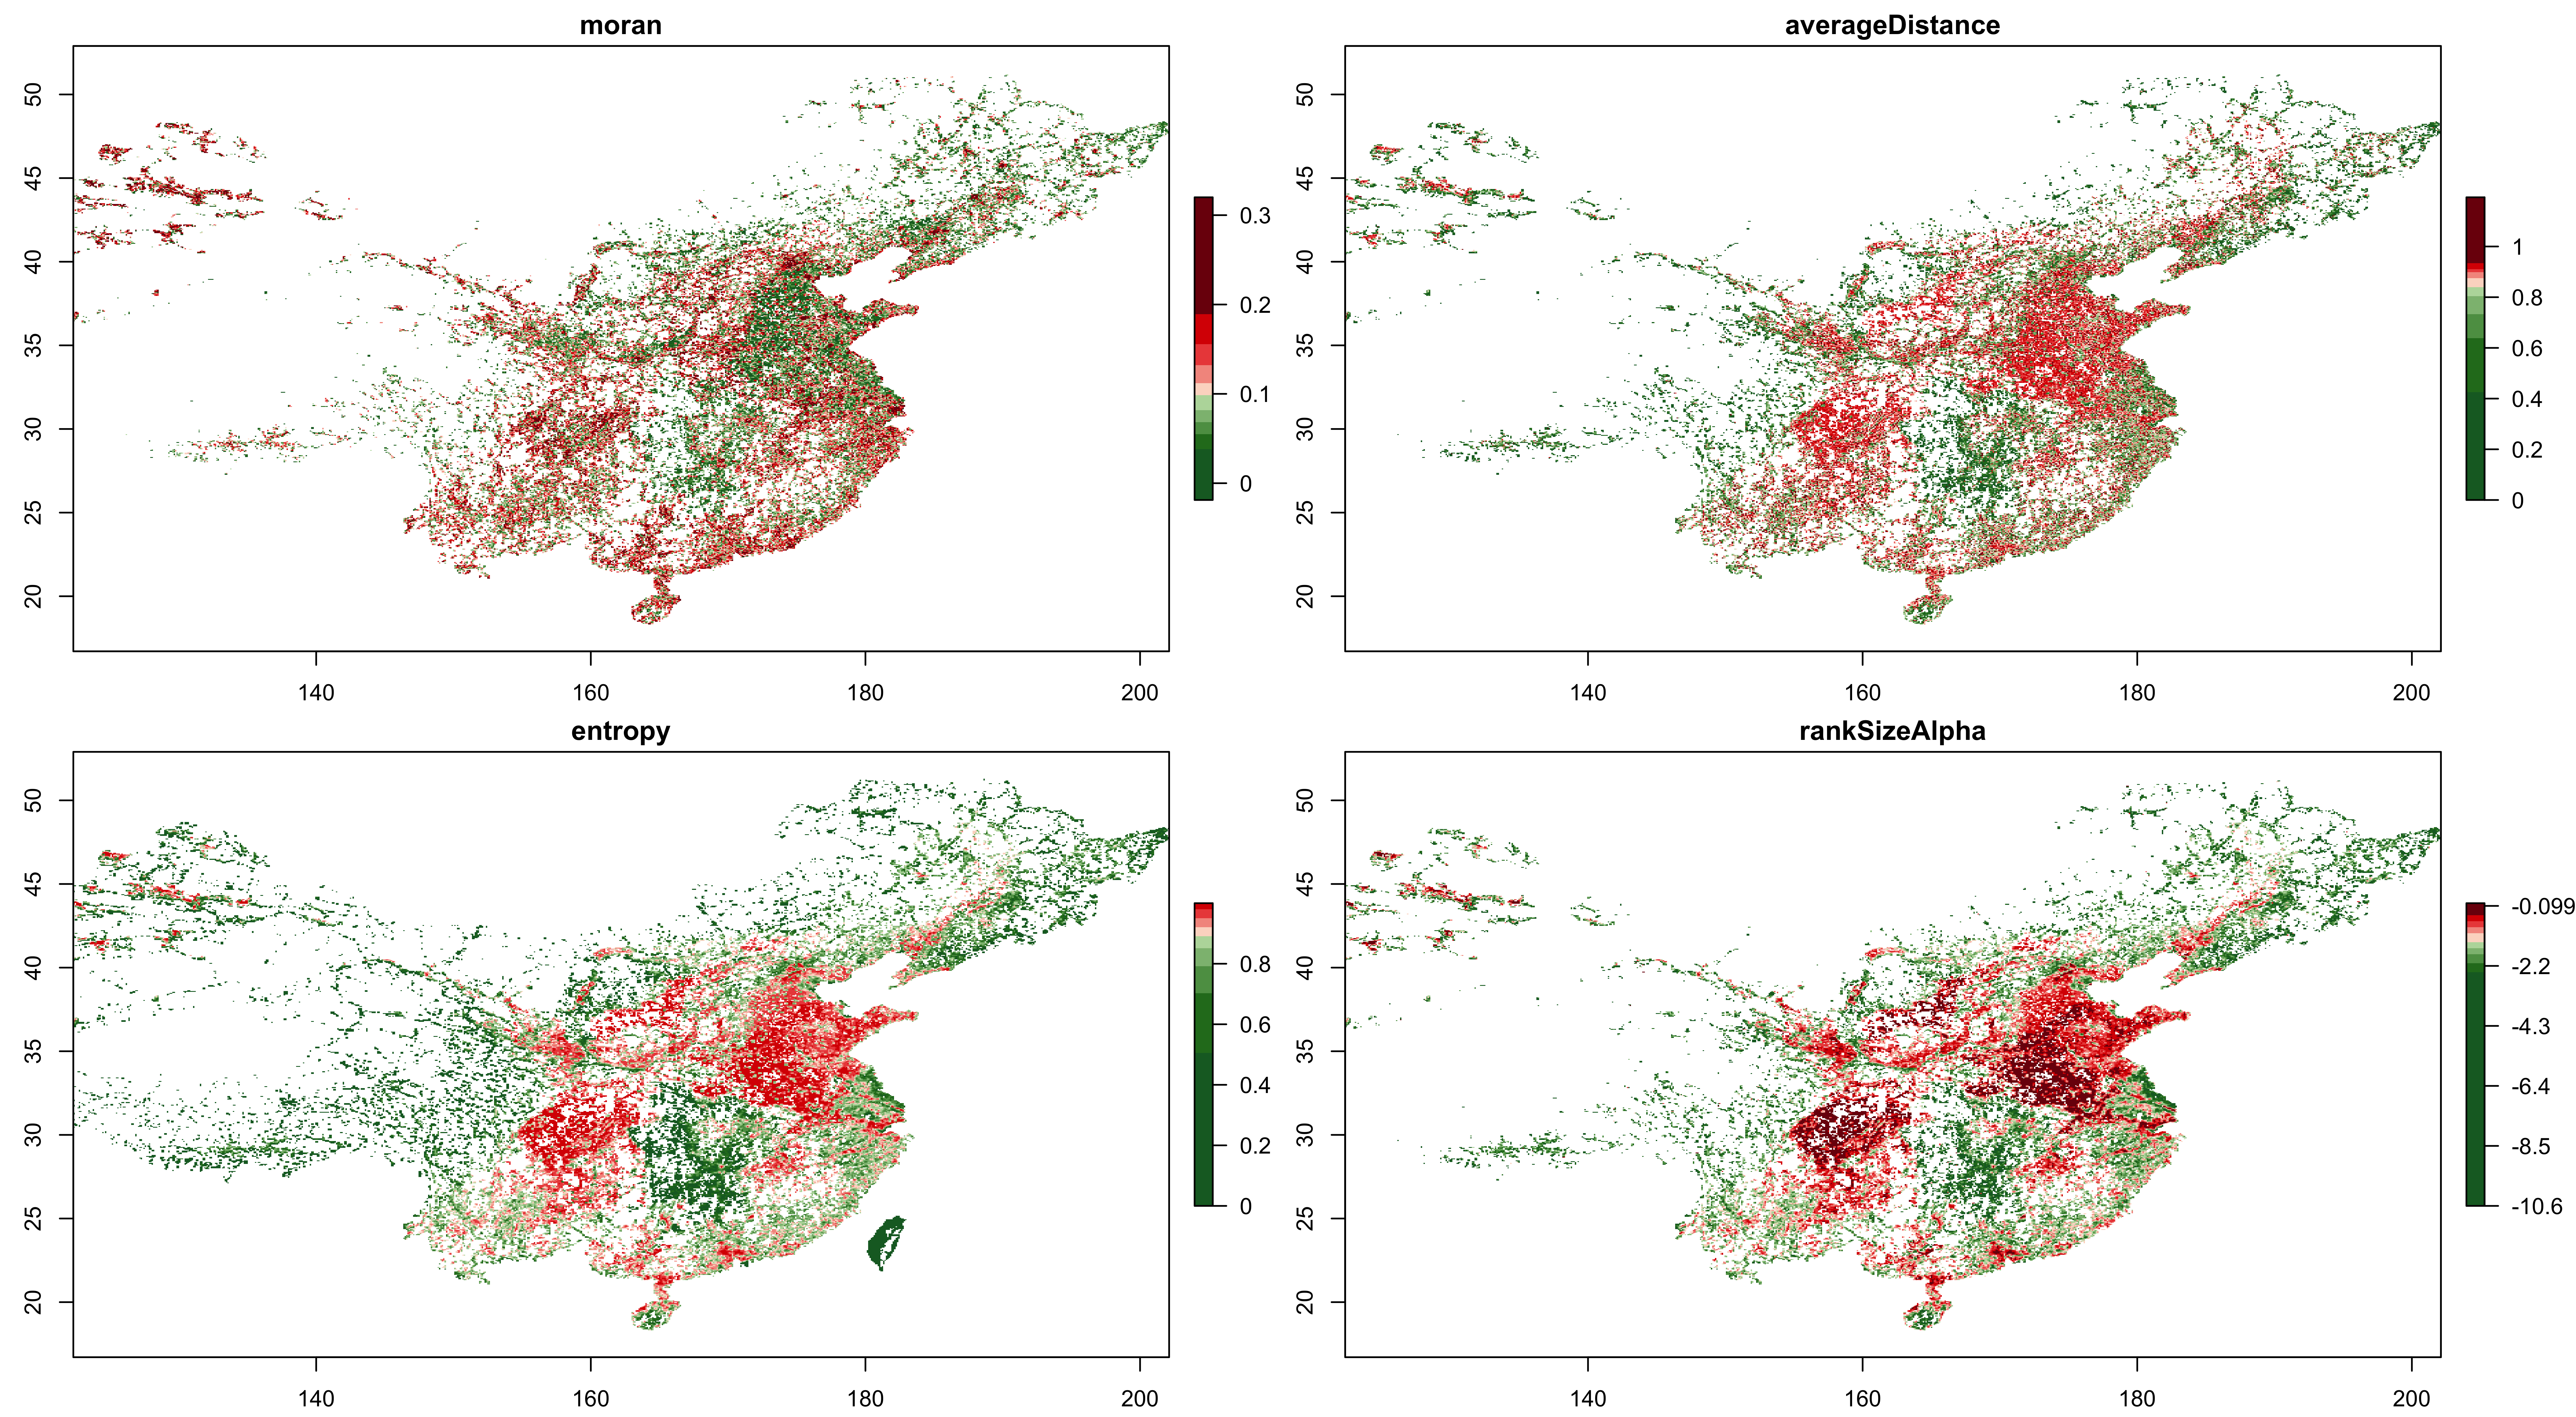
\includegraphics[width=\linewidth]{Figures/StaticCorrelations/CN_indics_morpho}
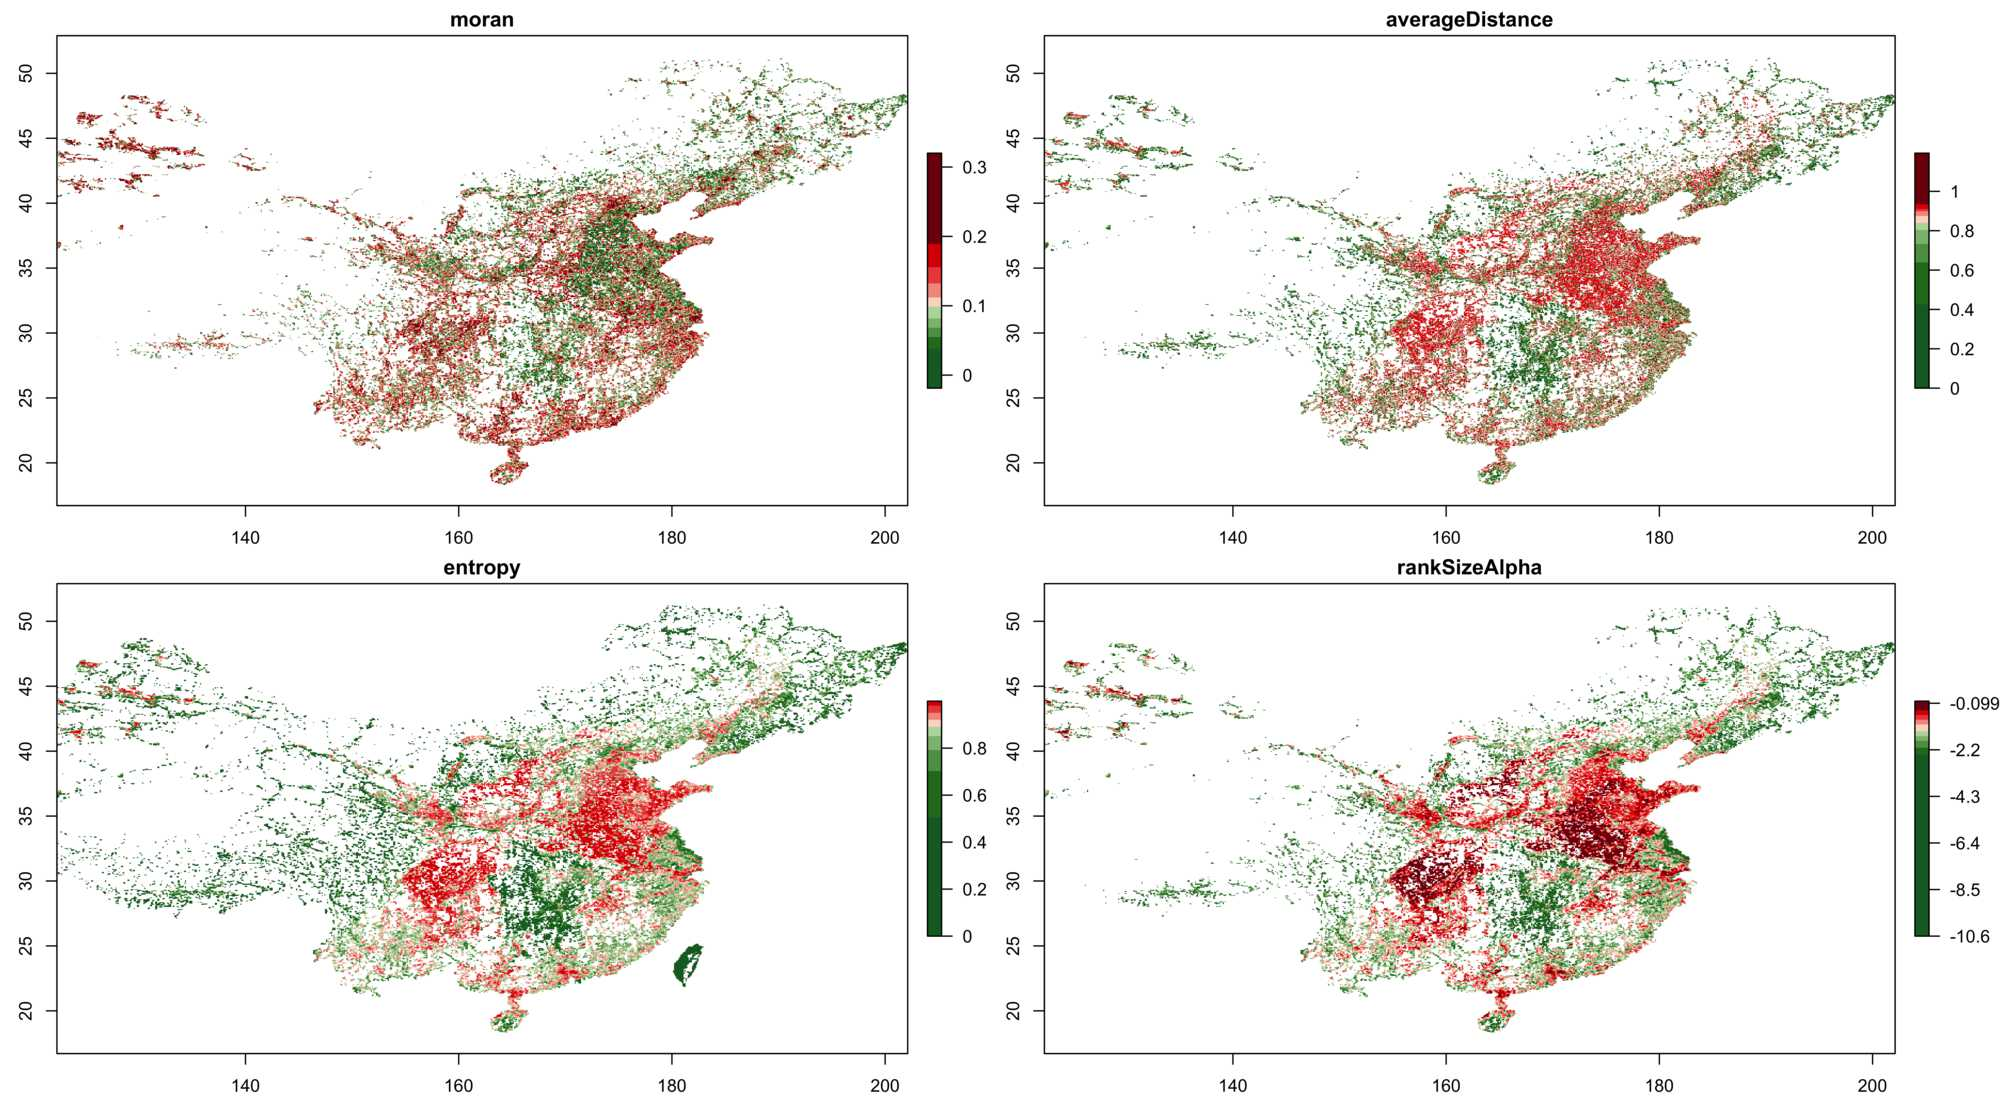
\includegraphics[width=\linewidth]{Figures/Final/A-staticcorrelations-morphocn.jpg}
\appcaption{\textbf{Morphological indicators for China.}\label{fig:app:staticcorrelations:morphocn}}{\textbf{Indicateurs morphologiques pour la Chine.}\label{fig:app:staticcorrelations:morphocn}}
\end{figure}
%%%%%%%%%%%%%%

%%%%%%%%%%%%%%%%%%%%%%%
\subsection{Road network}{Réseau routier}




%%%%%%%%%%%%%%%%%%%%%%%
\subsubsection{Network Simplification Algorithm}{Algorithme de Simplification du Réseau}

% data collected from http://download.geofabrik.de/europe.html : bosse pas sur le fichier world, huge.

Nous détaillons ici l'algorithme de simplification du réseau routier à partir des données OpenStreetMap. La logique générale est la suivante : (i) import des données par sélection et agrégation spatiale à la résolution du raster ; (ii) simplification pour conserver le réseau topologique uniquement, opérée en parallèle par \emph{split/merge}.


Les données OSM sont importées dans une base de données \texttt{pgsql} (extension \texttt{Postgis} pour la gestion des géométries et avoir des index spatiaux. L'import est fait en utilisant le logiciel \texttt{osmosis}~\cite{osmosis}, à partir d'une image en format compressé \texttt{pbf} de la base OpenStreetMap\footnote{Les dumps ont été récupérés à partir de \url{http://download.geofabrik.de}, en juillet 2016 pour l'Europe, et juillet 2017 pour la Chine.}. Nous filtrons à cette étape les liens (\texttt{ways}) qui possèdent le tag \texttt{highway}, et conservons les noeuds correspondants.


Le réseau est d'abord agrégé à une granularité de 100m pour pouvoir être utilisé de manière cohérente avec les grilles de population. Cela permet par ailleurs d'être robuste aux imperfections locales de codage ou données très locales manquantes. Pour cette étape, les routes sont filtrées sur un sous-ensemble de tags pertinents\footnote{Que nous prenons dans \texttt{motorway,trunk,primary,secondary,tertiary,unclassified,residential}.}. Pour l'ensemble des segments des lignes correspondantes, un lien est créé entre la cellule d'origine et de destination, avec longueur réelle calculée entre les centres des cellules et vitesse prise comme la vitesse de la ligne si elle est disponible.
  
La simplification est alors opérée de la façon suivante :
\begin{enumerate}
\item Network is simplified by iterative suppression of nodes with degree two, with keeping link speed and real length to their effective value.
\end{enumerate}

% \cite{2016arXiv161101890B} : interactive appli for network simplification



%\paragraph{Implementation}{Implémentation}
%A \texttt{PostGIS} database is used to store raw and simplified network, in order to perform efficient spatial requests, compared for example to initial \texttt{osm} data formats (\texttt{osm} or \texttt{pbf}). However the size of storage of data into this base is much higher (factor 10) so processing was parallelized between european countries. Consistence is ensured by the use of the same common density raster as simplification canvas. Final network is stored into the Postgis database for efficient indicator computation given a spatial extent.

%\paragraph{Sensitivity to simplification parameters}{Sensibilité aux paramètres de simplification}
%Sensitivity of indicators to raster resolution and to degree simplification algorithm must still be tested to ensure the relevance of data preprocessing.



% example of simpl stage
 %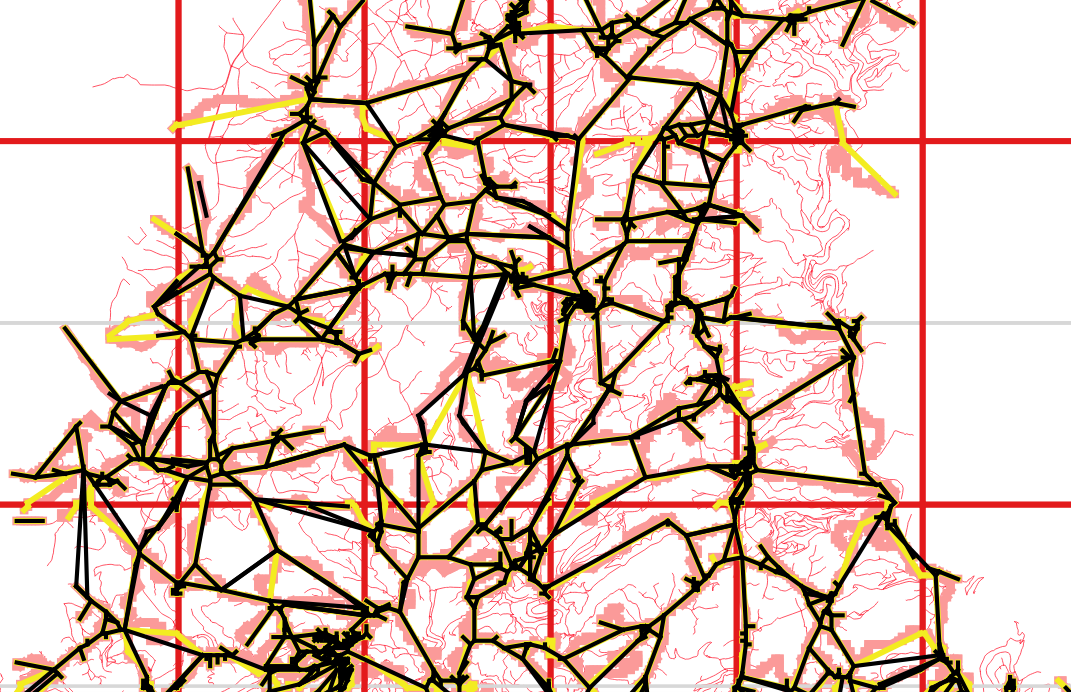
\includegraphics[width=\textwidth,height=0.5\textheight]{figures/ex_nw}




\subsubsection{Network Indicators}{Indicateurs de réseau}

Nous donnons en Fig.~\ref{fig:app:staticcorrelations:networkcn} un échantillon d'indicateurs de réseau pour la Chine.

%%%%%%%%%%%%%%
\begin{figure}
%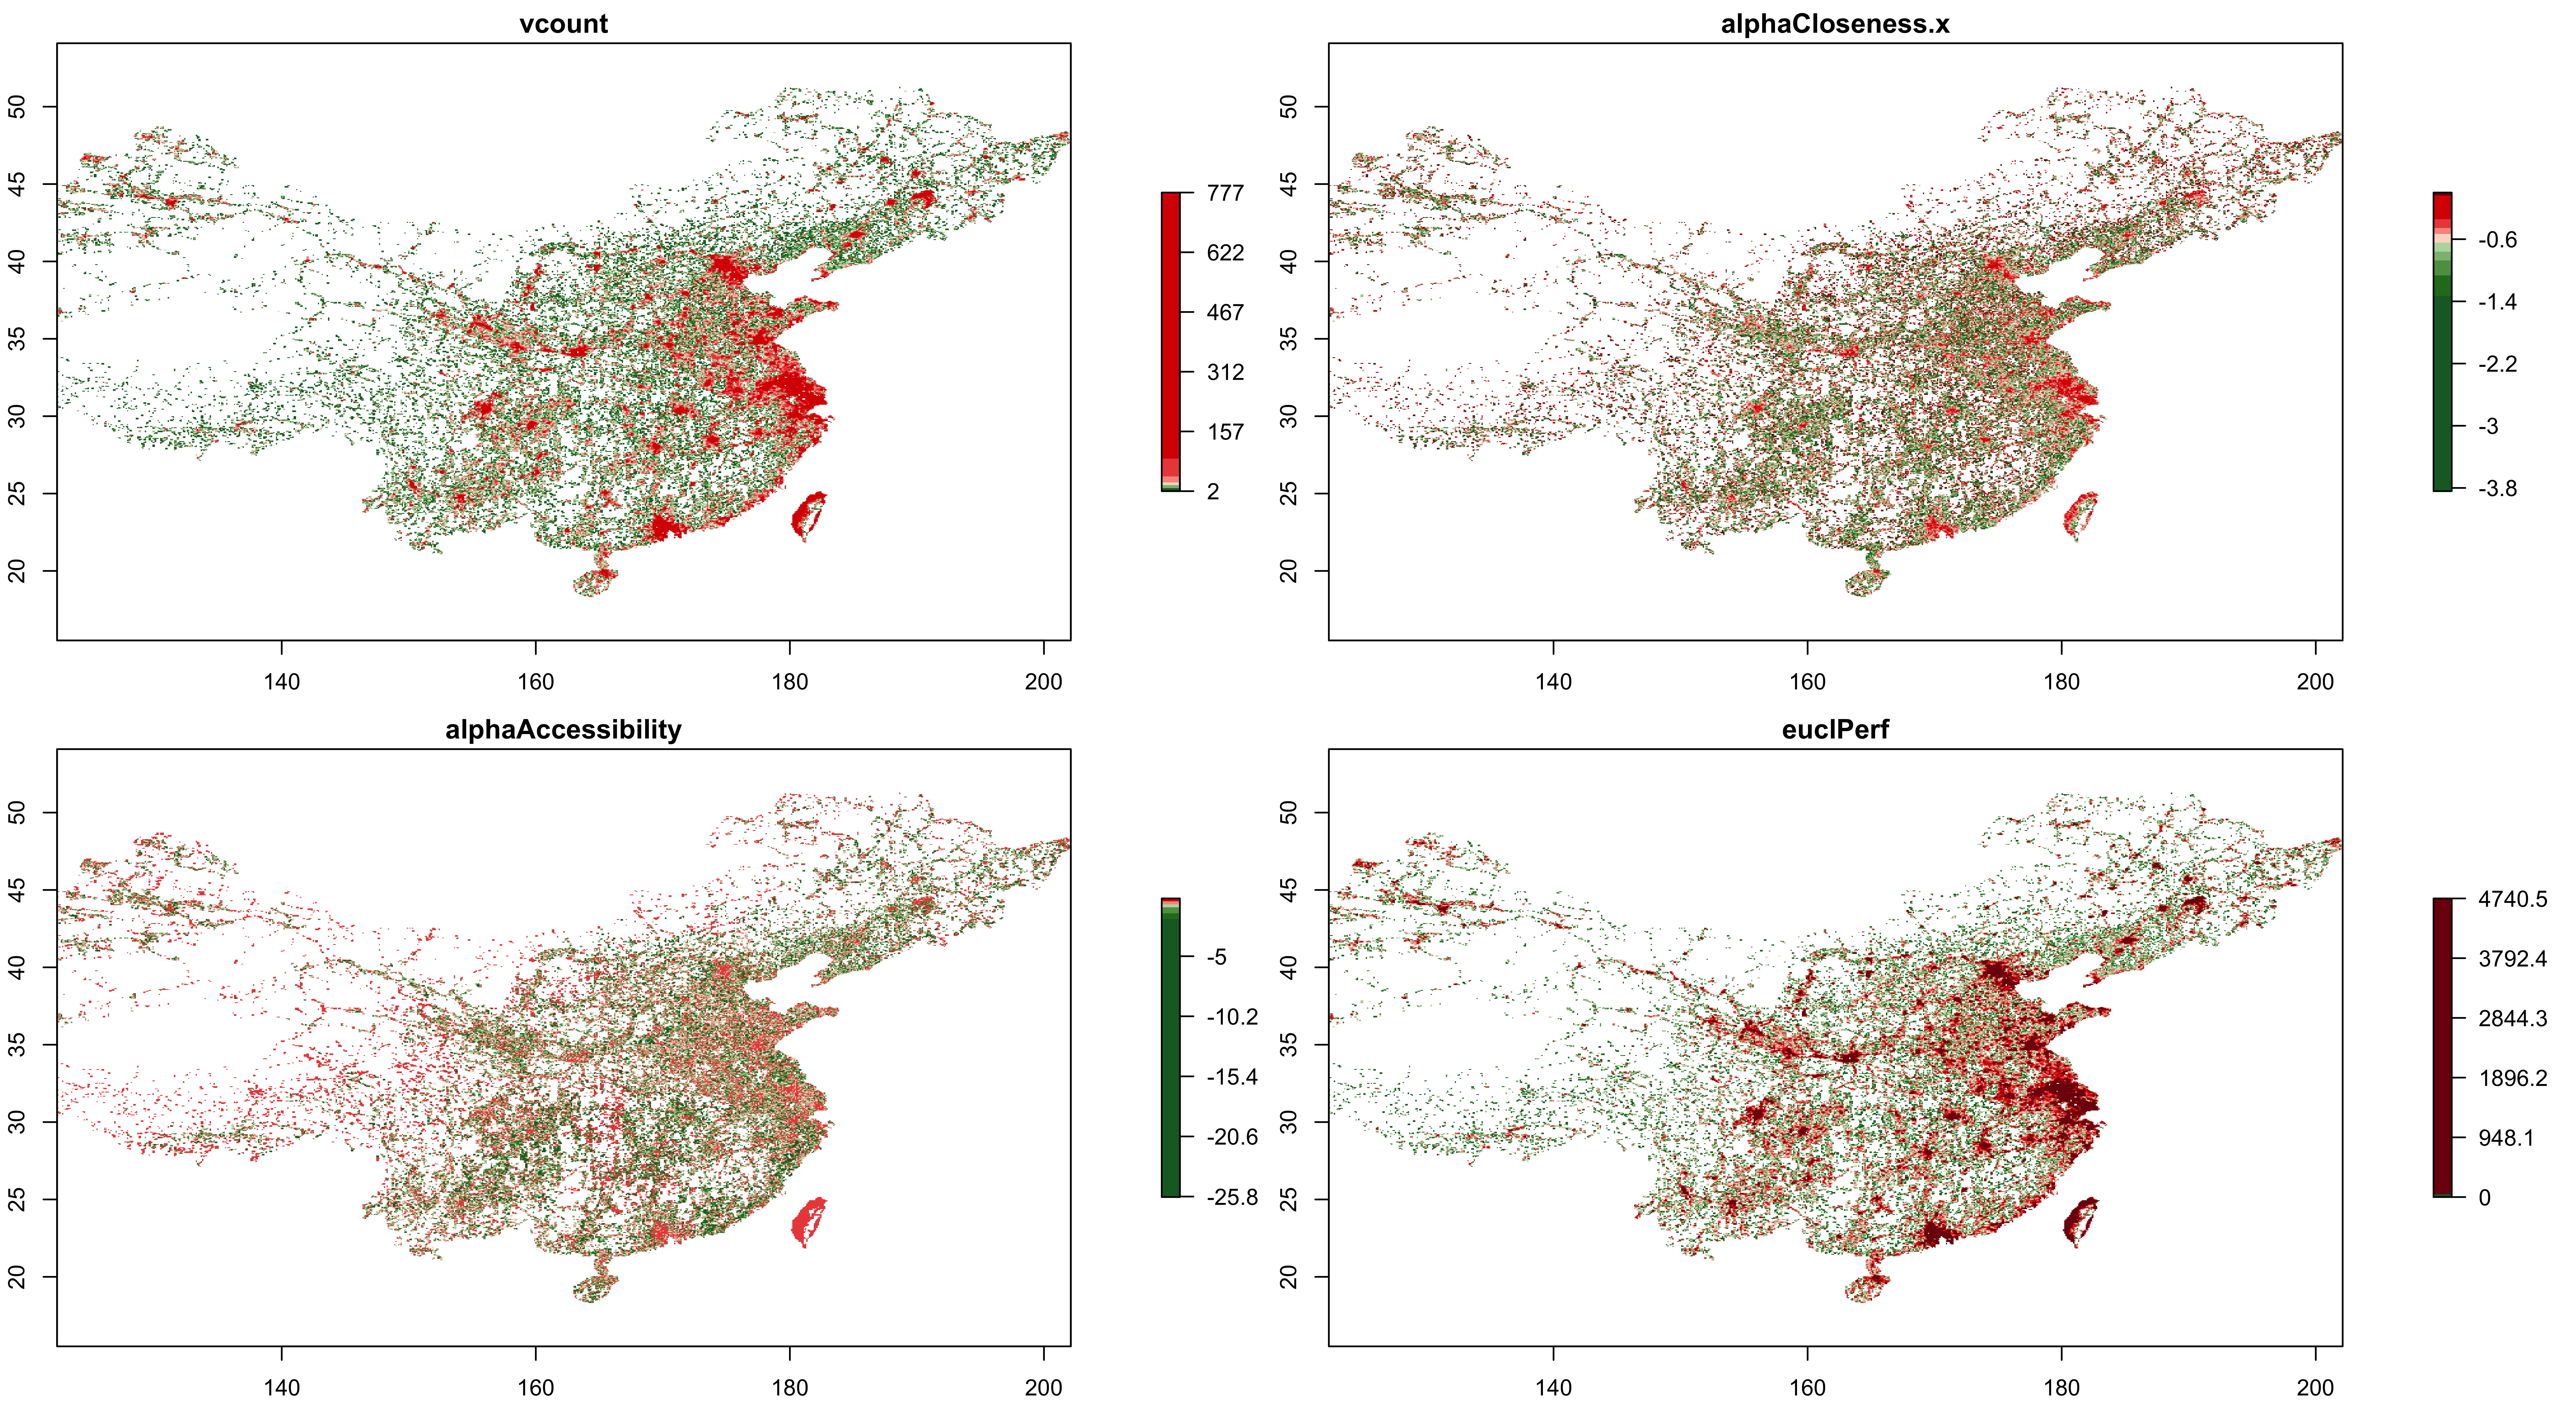
\includegraphics[width=\linewidth]{Figures/StaticCorrelations/CN_indics_network_selected}
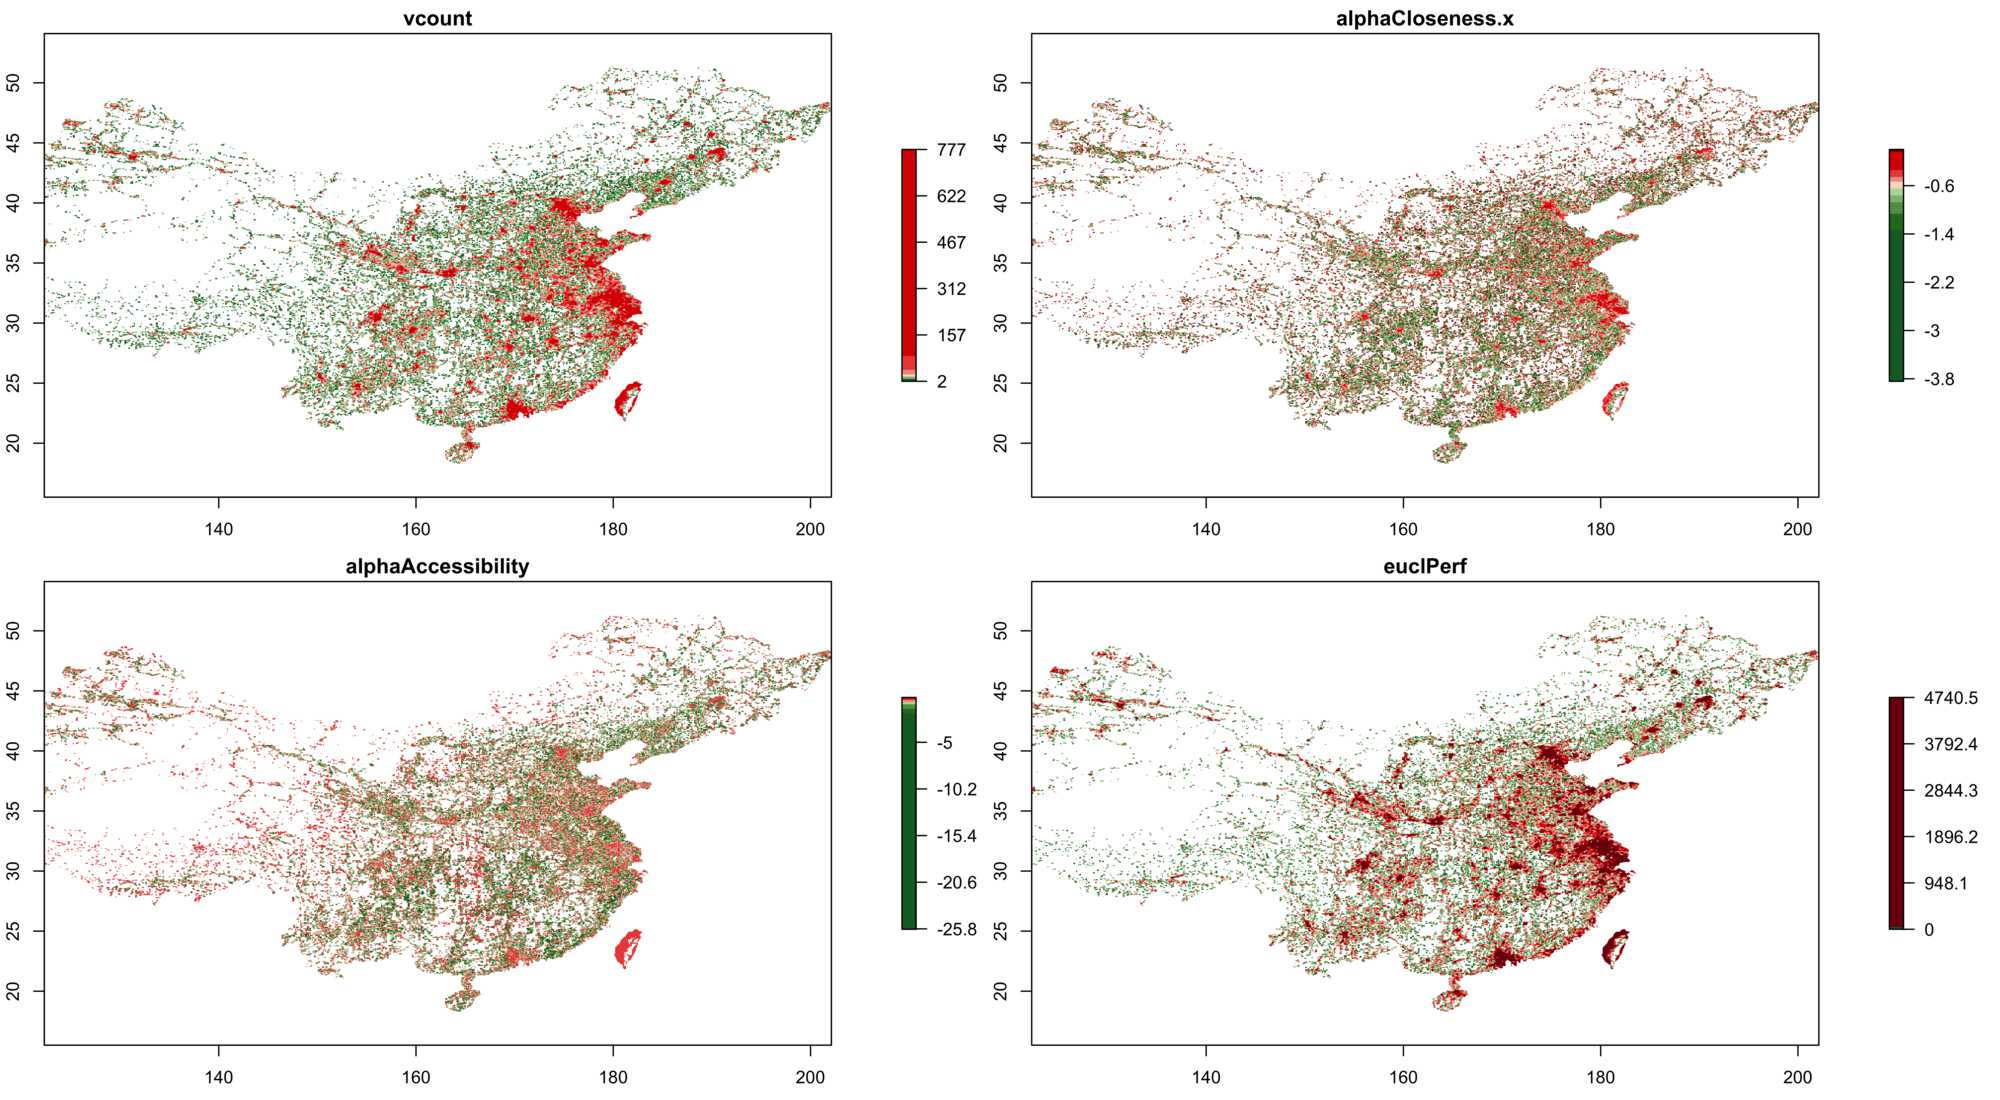
\includegraphics[width=\linewidth]{Figures/Final/A-staticcorrelations-networkcn.jpg}
\appcaption{\textbf{Network indicators for China.}\label{fig:app:staticcorrelations:networkcn}}{\textbf{Indicateurs de réseau pour la Chine.} Nous montrons une sélection d'indicateurs de réseau : nombre de noeuds $\left|V\right|$ (\texttt{vcount}), hiérarchie de \emph{closeness} $\alpha_{cl}$ (\texttt{alphaCloseness.x}), hiérarchie de l'accessibilité $\alpha_Z$ (\texttt{alphaAccessibility}), performance euclidienne $v_0$ (\texttt{euclPerf}).\label{fig:app:staticcorrelations:networkcn}}
\end{figure}
%%%%%%%%%%%%%%





%%%%%%%%%
%% -- ON HOLD --


%%%%%%%%%%%%%%%%%%%%%%%
%\subsection{Network Resilience}{Résilience des Réseaux}
%La description complète d'un réseau suppose la donnée d'une grande quantité d'information, puisque la moitié de la matrice d'adjacence est nécessaire dans le cas non-dirigé (matrice complète dans le cas dirigé). L'établissement de typologies, c'est à dire de sortes de classes d'équivalence topologiques au sens large, est une façon de voir les enjeux de la recherche actuelle sur les réseaux : existe-t-il des formes typiques de réseau, et comment les représenter dans une dimension réduite ? Relativement importante est la dimension épistémologique de cette interrogation fondamentale, qui peut sous certaines hypothèses être ramenée à l'opposition d'un réductionisme à une vision intrinsèque de la complexité. Si une classification systématique réductrice existe pour tout système complexe, alors les niveaux d'émergence supérieurs n'ont pas de signification propre. Il est paradoxal d'observer dans ce cas la position ambigüe de certains travaux de physiciens qui tiennent ce réductionisme comme un dogmatisme mais prétendent s'attaquer à des problèmes complexes typiques des systèmes socio-techniques.
%Les mesures de réseau globales comme nous avons vu en cours sont une façon de répondre partiellement à cette question de réduction dimensionnelle. En pratique, on veut être également capable de relier ces mesures à des propriétés pratiques du réseau, qui seront cruciales pour le design et le management de réseaux réels (par exemple réseaux techniques : transport d'électricité, internet ; réseaux de transport ; réseaux sociaux ; réseaux de villes ; etc.) : par exemple le coût, la résilience, la performance. Cet exercice propose de survoler ces deux questions fondamentales pour différents exemples de réseaux réels et synthétiques : illustrer dans un premier temps la signification concrète de différentes valeurs en relation à la topologie ``apparente'' du réseau ; dans un second temps explorer des liens potentiels entre mesures et propriétés afin de donner une idée d'une manière de caractériser la résilience.
%Cet exercice pourra paraître relativement simple mais est central pour une appréhension juste de la complexité des processus géographiques tels qu'ils occurrent dans toute leur réalité. La table~\ref{tab:measures} donne les valeurs d'indicateurs, pour certains types de réseaux. On fournit leur valeur moyenne et leur écart-type dans le cas de réseaux synthétiques aléatoires pour lesquels les mesures auront alors été estimées sur $b=500000$ répétitions des réseaux aléatoires.\footnote{qu'on fixe comme arbitraire. Le problème du nombre de répétitions nécessaires pour une convergence raisonnable des indicateurs statistiques et hors du champ de ce devoir, et d'ailleurs un problème ouvert pour la plupart des modèles de simulation complexes puisque qu'on sait établir des intervalles de confiances soit sous certaines hypothèses théoriques de distribution statistique soit par simulation (\emph{bootstrap}) ce qui ne réduit pas la complexité intrinsèque.} Pour les réseaux réels ou synthétiques non variables, une valeur seule est donnée, sachant que l'estimation de paramètres moyens dans des situations réelles est directement liée à la stationnarité spatio-temporelle des processus\footnote{et donc à leur ergodicité, i.e. à l'équivalence entre moyenne spatiale et moyenne temporelle}, ce qui est également une question ouverte concernant les systèmes spatiaux complexes. Les figures~\ref{fig:examples} et ~\ref{fig:real} illustre des exemples des réseaux considérés. Les questions suivantes portent sur une interprétation simple des mesures. Parmi les réseaux considérés, on étudie des réseaux routiers réels, dont la localisation spatiales est présentée en figure~\ref{fig:loc}, ainsi que des réseaux synthétiques.
%Les réseaux étudiés sont donc les suivants\footnote{chaque générateur synthétique a des paramètres propres, pour lesquels nous choisissons les valeurs par défaut suivantes : probabilité aléatoire d'Erdos-Renyi $p=0.005$ ; proportion de liens de la grille conservés $65\%$ ; attachement préférentiel : nouveau liens $m=10$, exposant $\alpha=1$, exposant de vieillissement $\beta = -2$, pas de vieillissement 100 ; nombre de feuille par branche de l'arbre $f=3$.} : 
%\begin{itemize}
%\item Réseau routiers réels (simplifiés à une résolution de 100m) : Paris, Ile-de-France, La Courtine (Creuse), Grand Lyon, London Metropolitan Area, Randstad
%\item Aléatoire (probabilité fixe d'établir un lien entre chaque paire de noeud)
%\item Attachement préférentiel (type Barabasi-Albert : les liens sont établis itérativement avec une probabilité proportionnelle au degré des noeuds)
%\item Grille perturbée (grille régulière dont on retire une proportion fixée de liens)
%\item Arbre (au nombre de feuilles par branche fixe)
%\end{itemize}

%Les mesures calculées pour un réseau $N=(V,E)$ sont celles décrites en~\ref{sec:staticcorrelations}.

%\begin{itemize}
%\item Statistiques descriptives : nombre de noeuds $\left|V\right|$ et nombre de liens $\left|E\right|$
%\item Densité $\gamma$
%\item Degré moyen $\bar{d}$
%\item Diamètre\footnote{pour toutes les mesures liées au plus courts chemins, les distances topologiques et non pondérées ont été prises en compte, afin de permettre la comparabilité des réseaux réels et des réseaux synthétiques. Pour une comparabilité des réseaux réels ayant des couvertures géographiques d'étendue significativement différentes, il faut normaliser par le diamètre.} $\delta$
%\item Centralité d'intermédiarité $b$ : s'agissant d'une mesure locale (associée ici aux liens), on considère sa moyenne $<b>$ et son niveau de hiérarchie\footnote{donné par la pente de la regression linéaire d'un fit brutal d'une loi rang-taille : $\log{b_i} = \beta + \alpha\cdot \log i$ où les $b_i$ sont triés par ordre decroissants.} $\alpha\left[b\right]$
%\item Centralité de proximité $c$ : de même on calcule $<c>$ et $\alpha\left[c\right]$
%\item Efficacité $e = \frac{2}{n\cdot (n-1)} \sum_{i<j} \frac{1}{d_{ij}}$ avec $d_{ij}$ distance topologique entre $i$ et $j$
%\item Coefficient de clustering $t$, qui donne la probabilité que les voisins d'un noeud soient connectés
%\item Modularité $\mu$ qui donne une mesure plus générale de la structure en communauté du graphe
%\end{itemize}


%
%%%%%%%%%%%%%%%
%\begin{table}
%\hspace{-1cm}
%\begin{tabular}{c|c|c|c|c|c|c|c|c|c|c|c|c}
%\hline
%Réseau & $\left|V\right|$ & $\left|E\right|$ & $\gamma$ & $\bar{d}$ & $\delta$ & $<b>$ \\\hline
%Aléatoire & $1000$ & $2498 \pm 50 $ & $0.005 \pm 1\cdot 10^{-4} $ & $5 \pm 0.1 $ & $9 \pm 0.59 $ & $0.0018 \pm 5.4\cdot 10^{-5} $\\\hline
%Att. Préf. & $1000$ & $4579 \pm 21 $ & $0.0092 \pm 4.3\cdot 10^{-5} $ & $9.2 \pm 0.043 $ & $7 \pm 0.18 $ & $0.00084 \pm 8.6\cdot 10^{-6} $\\\hline
%Grille & $499\pm 3.7 $ & $624$ & $0.005 \pm 7.5\cdot 10^{-5} $ & $2.5 \pm 0.019 $ & $53 \pm 4.5 $ & $0.03 \pm 0.0027 $\\\hline
%Arbre & $1000$ & $999$ & $0.002$ & $2$ & $12$ & $0.0099$\\\hline
%Ile-de-France & $\left|V\right|$ & $\left|E\right|$ & $\gamma$ & $\bar{d}$ & $\delta$ & $<b>$\\\hline
%Paris & $\left|V\right|$ & $\left|E\right|$ & $\gamma$ & $\bar{d}$ & $\delta$ & $<b>$\\\hline
%Grand Lyon & $\left|V\right|$ & $\left|E\right|$ & $\gamma$ & $\bar{d}$ & $\delta$ & $<b>$\\\hline
%La Courtine & $\left|V\right|$ & $\left|E\right|$ & $\gamma$ & $\bar{d}$ & $\delta$ & $<b>$\\\hline
%Randstad & $\left|V\right|$ & $\left|E\right|$ & $\gamma$ & $\bar{d}$ & $\delta$ & $<b>$\\\hline
%London& $\left|V\right|$ & $\left|E\right|$ & $\gamma$ & $\bar{d}$ & $\delta$ & $<b>$\\\hline
%\end{tabular}
%\bigskip
%\hspace{-1cm}
%\begin{tabular}{c|c|c|c|c|c|c}
%\hline
%Réseau & $\alpha \left[b\right]$ & $<c>$ & $\alpha\left[c\right]$ & $e$ & $t$ & $\mu$\\\hline
%Aléatoire & $-0.29 \pm 0.0092 $ & $0.46 \pm 0.68 $ & $-0.076 \pm 0.032 $ & $0.24 \pm 0.003 $ & $0.005 \pm 0.0011 $ & $0.45 \pm 0.0072 $\\\hline
%Att. Préf. & $-0.63 \pm 0.015 $ & $0.26 \pm 0.0021 $ & $-0.062 \pm 0.0022 $ & $0.28 \pm 0.0018 $ & $0.079 \pm 0.0028 $ & $0.66 \pm 0.0082 $\\\hline
%Grille & $-1.2 \pm 0.077 $ & $7.3 \pm 3.5 $ & $-0.99 \pm 0.31 $ & $0.072 \pm 0.0032 $ & $0$ & $0.87 \pm 0.0058 $\\\hline
%Arbre & $-1$ & $0.1$ & $-0.094$ & $0.11$ & $0$ & $0.93$
%\end{tabular}
%\caption[][]{}{Valeurs de mesures de réseaux pour différents exemples typiques réels et synthétiques \label{tab:measures}}
%\end{table}
%%%%%%%%%%%%%%%
%

%
%\paragraph{}{Formes Urbaines et indicateurs de réseaux}
%
%Commentez qualitativement les différentes formes des systèmes territoriaux observées. On pourra par exemple se poser la question de la polycentricité d'une Méga-région Urbaine. Reliez ces observations aux valeurs prises par les indicateurs que vous jugez pertinents.
%
%\paragraph{}{Interprétation des Indicateurs}
%
%Pour les réseaux synthétiques, commentez les valeurs prises par les indicateurs. Lesquelles étaient intuitivement attendues ? Dans quelle mesure est-on capable de caractériser et discriminer chaque type de réseau. De quel réseau synthétique s'attend-on à ce que les réseaux réels soient les plus proches ? Peut-on le confirmer par les indicateurs ?
%
%
%Nous proposons à présent de tenter une caractérisation de la résilience des réseau. La définition utilisée prend en compte la capacité du réseau à rester performant face à la rupture de lien, comme proposé par~\cite{ash2007optimizing}. On considère la rupture aléatoire d'une proportion fixée $\alpha$ de liens, et on note $N_{\alpha}$ le réseau résultant de la suppression à partir du réseau $N$. L'indicateur de résilience au niveau $\alpha$ est alors défini par $r = \mathbb{E} \left[\Delta_{\alpha} e \right] = \mathbb{E}\left[ e\left(N_{\alpha}\right) - e\left(N\right)\right]$. On peut définir de même les variations des autres indicateurs. La structure de covariance des différentes variations, et en particulier la correlation avec la résilience, est un moyen indirect de caractériser la résilience, au sens de quel type de propriété permet au réseau d'augmenter sa résilience. La table~\ref{tab:corr} donne pour chaque réseau aléatoire les correlations estimées $\rho\left[X\right] = \hat{\rho}\left[\Delta_{\alpha} e,\Delta_{\alpha} X\right]$ où l'estimateur $\hat{\rho}$ est calculé en pratique sur une plage de valeurs pour $\alpha$ (de 0.5 à 0.95 par 0.05) et sur un nombre de répétitions fixé ($b=$, en faisant l'hypothèse que répéter sur le réseau est équivalent à répéter sur la suppression des liens).
%
%
%%%%%%%%%%%%%%%
%\begin{table}
%\begin{tabular}{c|c|c|c|c|c|c|c|c|c|c|c|c}
%\hline
%Réseau & $\left|V\right|$ & $\left|E\right|$ & $\gamma$ & $\bar{d}$ & $\delta$ & $<b>$ & $\alpha \left[b\right]$ & $<c>$ & $\alpha\left[c\right]$ & $e$ & $t$ & $\mu$\\\hline
%Aléatoire & $\left|V\right|$ & $\left|E\right|$ & $\gamma$ & $\bar{d}$ & $\delta$ & $<b>$ & $\alpha \left[b\right]$ & $<c>$ & $\alpha\left[c\right]$ & $e$ & $t$ & $\mu$\\\hline
%Attachement Préférentiel & $\left|V\right|$ & $\left|E\right|$ & $\gamma$ & $\bar{d}$ & $\delta$ & $<b>$ & $\alpha \left[b\right]$ & $<c>$ & $\alpha\left[c\right]$ & $e$ & $t$ & $\mu$\\\hline
%Grille Perturbée & $\left|V\right|$ & $\left|E\right|$ & $\gamma$ & $\bar{d}$ & $\delta$ & $<b>$ & $\alpha \left[b\right]$ & $<c>$ & $\alpha\left[c\right]$ & $e$ & $t$ & $\mu$\\\hline
%\end{tabular}
%\caption[][]{}{Correlations estimées \label{tab:corr}}
%\end{table}
%%%%%%%%%%%%%%%
%
%
%
%\paragraph{}{Caractérisation de la résilience}
%
%Commentez à partir de la table des corrélations, pour les différents types de réseau, les facteurs influençant la résilience. Quel enseignement peut-on en tirer pour la conception de réseaux techniques par exemple ?
%
%
%
%\paragraph{}{Résilience Dynamique et Topologie}
%
%Les approches à la notion de résilience sont diverses et complémentaires. L'aspect dynamique, au sens par exemple du temps nécessaire au système pour retrouver son état initial après perturbation, est particulièrement intéressant pour les systèmes urbains. Dans le cas de réseaux où les noeuds ont leur dynamique propre, les solutions pour une définition robuste et universelle sont très récentes, comme celle proposée par~\cite{Gao:2016ty}.
%
%
%Vous semble-t-il simple, dans le cas de dynamiques couplées au sein d'un réseau, d'isoler la contribution de la topologie du réseau de celle des dynamiques propres à la dynamique générale ? Dans quelle mesure serait-il alors complexe de quantifier la résilience dynamique dans une dimension réduite ?
%
%





%%%%%%%%%%%%%%
%\begin{figure}
%\centering
%\includegraphics[width=0.45\textwidth,height=0.3\textheight]{figures/random_lowres.png}
%\includegraphics[width=0.45\textwidth,height=0.3\textheight]{figures/lattice.png}\\
%\includegraphics[width=0.45\textwidth,height=0.3\textheight]{figures/pa-age_lowres.png}
%\includegraphics[width=0.45\textwidth,height=0.3\textheight]{figures/tree_lowres.png}
%\appcaption{Synthetic Networks}{Représentation d'instances des exemples synthétiques de réseaux. Dans l'ordre de haut en bas et de droite à gauche : réseau aléatoire, grille perturbée, attachement préférentiel, arbre.\label{fig:examples}}
%\end{figure}
%%%%%%%%%%%%%%

%%%%%%%%%%%%%%
%\begin{figure}
%\includegraphics[width=0.45\textwidth,height=0.3\textheight]{figures/idf_lowres.png}
%\includegraphics[width=0.45\textwidth,height=0.3\textheight]{figures/paris_lowres.png}\\
%\includegraphics[width=0.45\textwidth,height=0.3\textheight]{figures/lyon_lowres.png}
%\includegraphics[width=0.45\textwidth,height=0.3\textheight]{figures/lacourtine_lowres.png}\\
%\includegraphics[width=0.45\textwidth,height=0.3\textheight]{figures/randstad_lowres.png}
%\includegraphics[width=0.45\textwidth,height=0.3\textheight]{figures/londonM25_lowres.png}\\
%\appcaption{Real networks}{Réseaux routiers réels étudiés. Dans l'ordre de haut en bas et de droite à gauche : Ile-de-France, Paris, Grand Lyon, La Courtine, Randstad, London Metropolitan Area\label{fig:real}}
%\end{figure}
%%%%%%%%%%%%%%

%%%%%%%%%%%%%%
%\begin{figure}
%\centering
%\includegraphics[width=0.8\textwidth]{figures/areas}
%\appcaption{Localisation of networks}{Localisation Géographique des réseaux réels étudiés.}
%\label{fig:loc}
%\end{figure}
%%%%%%%%%%%%%%


% questions :
% - commentaires sur mesures ?
% - intuitivement, le plus sensible aux perturbations ?
% - matrice des correlations pour chaque type : lecture ; interpretation
% - comment mesurer correlations sur réseaux réels ?
% - vers une mesure dynamique de la résilience : question conceptuelle sur séparation dynamique/topologie - évoquer papier barabasi ?





\subsection{Sensitivity to resolution}{Sensibilité à la résolution}


\bpar{}{
Nous évaluons ici la sensibilité des divers indicateurs à la taille de la grille. Nous montrons en Fig.~\ref{fig:app:staticcorrelations:sensitivity-maps-morpho} les indicateurs morphologiques et en Fig.~\ref{fig:app:staticcorrelations:sensitivity-maps-morpho} certains indicateurs de réseau, cartographiés pour la France, pour des tailles différentes de grille. Les tailles données ici, en écho à celle de 50km utilisée dans les résultats principaux, sont dans des ordres de grandeur équivalents : nous testons des fenêtres de taille 30km et 60km. Les décalages sont à chaque fois de la moitié de la fenêtre (15km et 50km respectivement). Il est possible de voir ``à l'oeil'' que certains indicateurs sont peu sensibles, le changement d'échelle ressemblant à un lissage du champ le plus fin : par exemple dans le cas morphologique pour l'indice de Moran, l'entropie et la hiérarchie. La distance moyenne, en fait très bruitée à l'échelle la plus faible, est nécessairement sensible à l'agrégation, ce qui est consistant avec une sensibilité attendue au lissage. Les indicateurs de réseau sont relativement robustes à la taille de la fenêtre.
}

\bpar{}{
Cette comparaison, d'une part est à prendre avec précaution de par la non-comparabilité directe des échelles pour les indicateurs, et d'autre part reste limitée. Nous proposons alors une méthode pour quantifier la variabilité des indicateurs à la taille de la fenêtre. Soit $X_D$ et $X_d$ deux champs spatiaux correspondant à deux échelles spatiales $D > d$ (qu'on prend comme des distances caractéristiques), qu'on suppose discrets en des points respectifs $\left(\vec{x}_i^{(D)}\right)_{1 \leq i \leq N_D}$ et $\left(\vec{x}_j^{(d)}\right)_{1 \leq i \leq N_d}$. L'idée est de comparer un lissage du champ le plus fin au champ le moins fin : si la corrélation entre ces deux valeurs est forte, il est possible de passer d'un champ à l'autre par agrégation et l'échelle de calcul n'influe ainsi pas autrement que sur la résolution finale. Soit $W_{ij} = \left( \exp{ - d_{ij} / d_0} \right)_{ij}$ une matrice de poids spatiaux calculée par les distances euclidiennes $d_{ij}$ entre les points $\vec{x}_i^{(D)}$ et $\vec{x}_j^{(d)}$. Alors avec $W'_{ij} = W_{ij} / \sum_j W_{ij}$, on peut calculer le lissage spatial de $X_d$ aux points $\vec{x}_i^{(D)}$, par le produit matriciel
\[
\tilde{X}_d (\vec{x}_i^{(D)}) = W' \ast \vec{x}_j^{(d)}
\]

La corrélation est alors donnée par $\rhob{\tilde{X}_d}{X_D}$ évaluée sur l'ensemble des points $\vec{x}_i^{(D)}$.
}


\bpar{}{
La Fig.~\ref{fig:app:staticcorrelations:sensitivity-corrs} donne les variations de la corrélation pour l'ensemble des couples $(D,d)$
}



%% maps

%%%%%%%%%%%%
\begin{figure}
	% Figures/StaticCorrelations/indics_morpho_areasize60_offset30_factor0.5.png
	% Figures/StaticCorrelations/indics_morpho_areasize200_offset100_factor0.5.png
	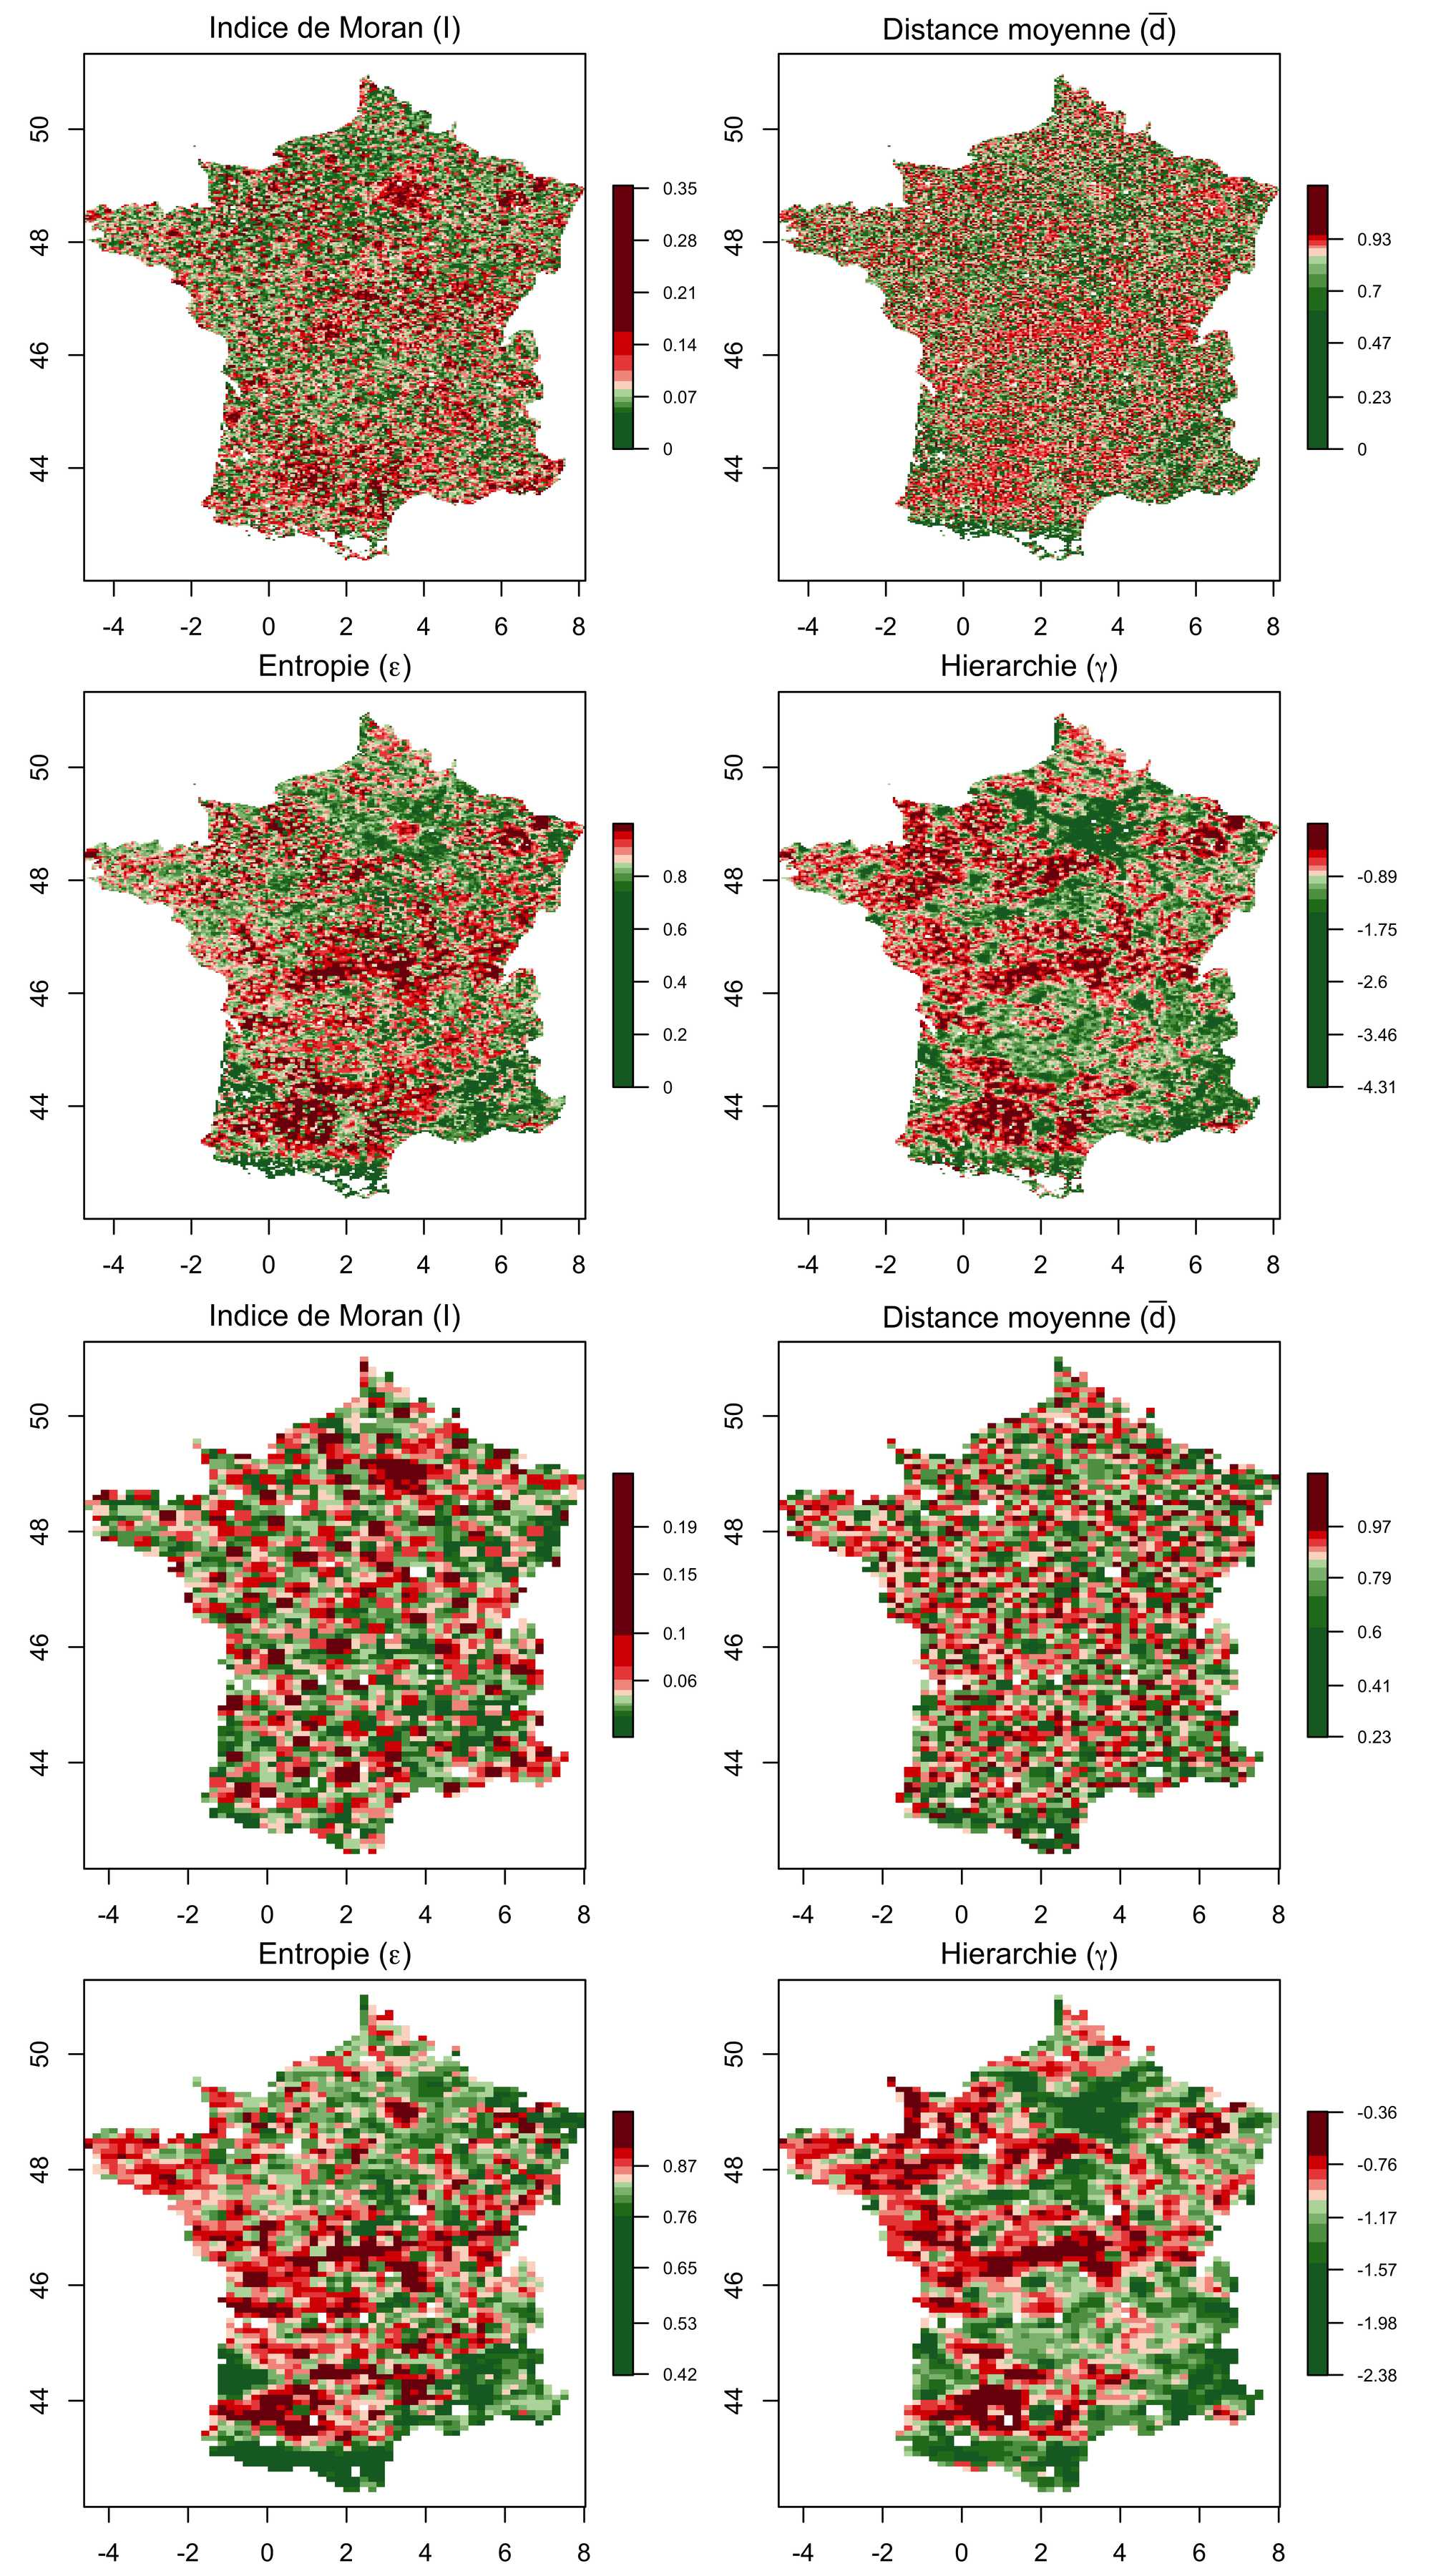
\includegraphics[width=\linewidth,height=0.95\textheight]{Figures/Final/A-staticcorrelations-sensitivity-maps-morpho.jpg}
	\appcaption{\label{fig:app:staticcorrelations:sensitivity-maps-morpho}}{\textbf{Indicateurs morphologiques pour différentes tailles de grille.} Les 4 premières cartes montrent les indicateurs calculés avec une fenêtre de taille 30km, les 4 dernières avec une fenêtre de taille 100km.\label{fig:app:staticcorrelations:sensitivity-maps-morpho}}
\end{figure}
%%%%%%%%%%%%


%%%%%%%%%%%%
\begin{figure}
	% Figures/StaticCorrelations/indics_network_areasize60_offset30_factor0.5.png
	% Figures/StaticCorrelations/indics_network_areasize200_offset100_factor0.5.png
	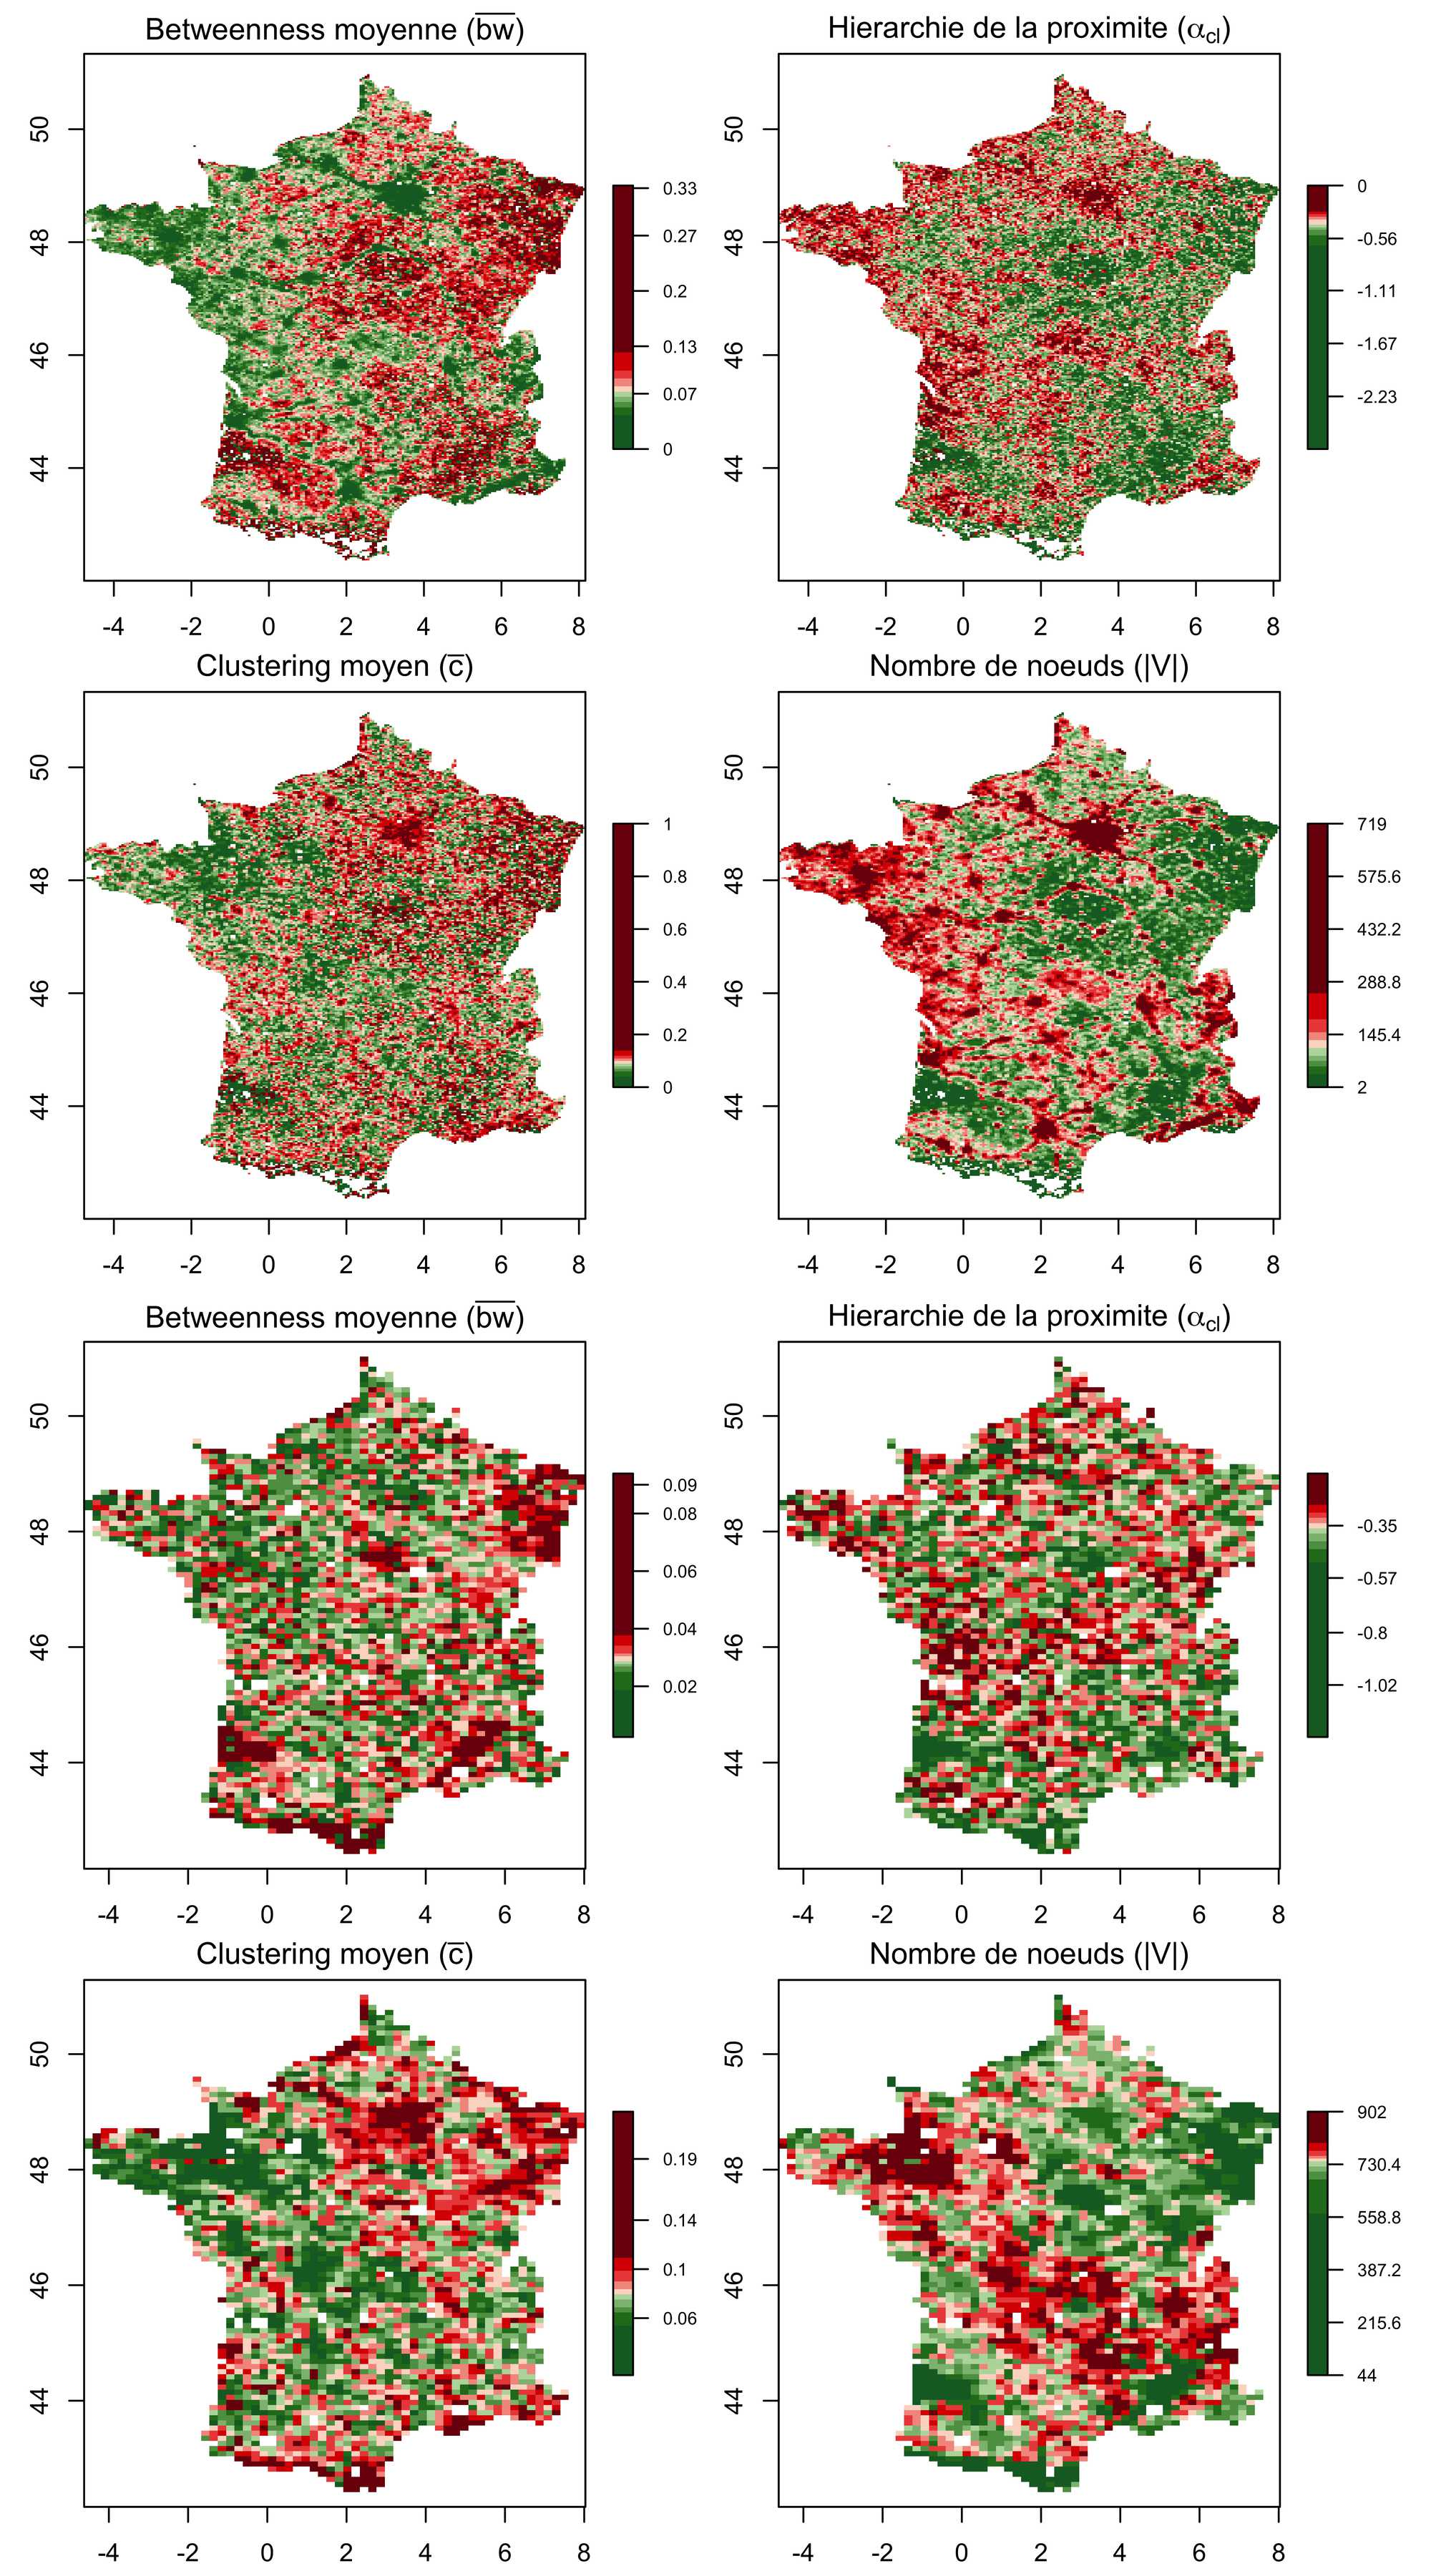
\includegraphics[width=\linewidth,height=0.95\textheight]{Figures/Final/A-staticcorrelations-sensitivity-maps-network.jpg}
	\appcaption{\label{fig:app:staticcorrelations:sensitivity-maps-network}}{\textbf{Echantillon des indicateurs de réseau pour différentes tailles de grille.} Les 4 premières cartes montrent les indicateurs calculés avec une fenêtre de taille 30km, les 4 dernières avec une fenêtre de taille 100km.\label{fig:app:staticcorrelations:sensitivity-maps-network}}
\end{figure}
%%%%%%%%%%%%


%% smoothed correlation

%%%%%%%%%%%%
\begin{figure}
	% Figures/StaticCorrelations/sensit_morpho_low60_high100.png
	% Figures/StaticCorrelations/sensit_network_low60_high100.png
	% Figures/StaticCorrelations/sensit_morpho_low60_high200.png
	% Figures/StaticCorrelations/sensit_network_low60_high200.png
	% Figures/StaticCorrelations/sensit_morpho_low100_high200.png
	% Figures/StaticCorrelations/sensit_network_low100_high200.png
	% Figures/StaticCorrelations/sensit_morpho_crossed.png
	% Figures/StaticCorrelations/sensit_network_crossed.png
	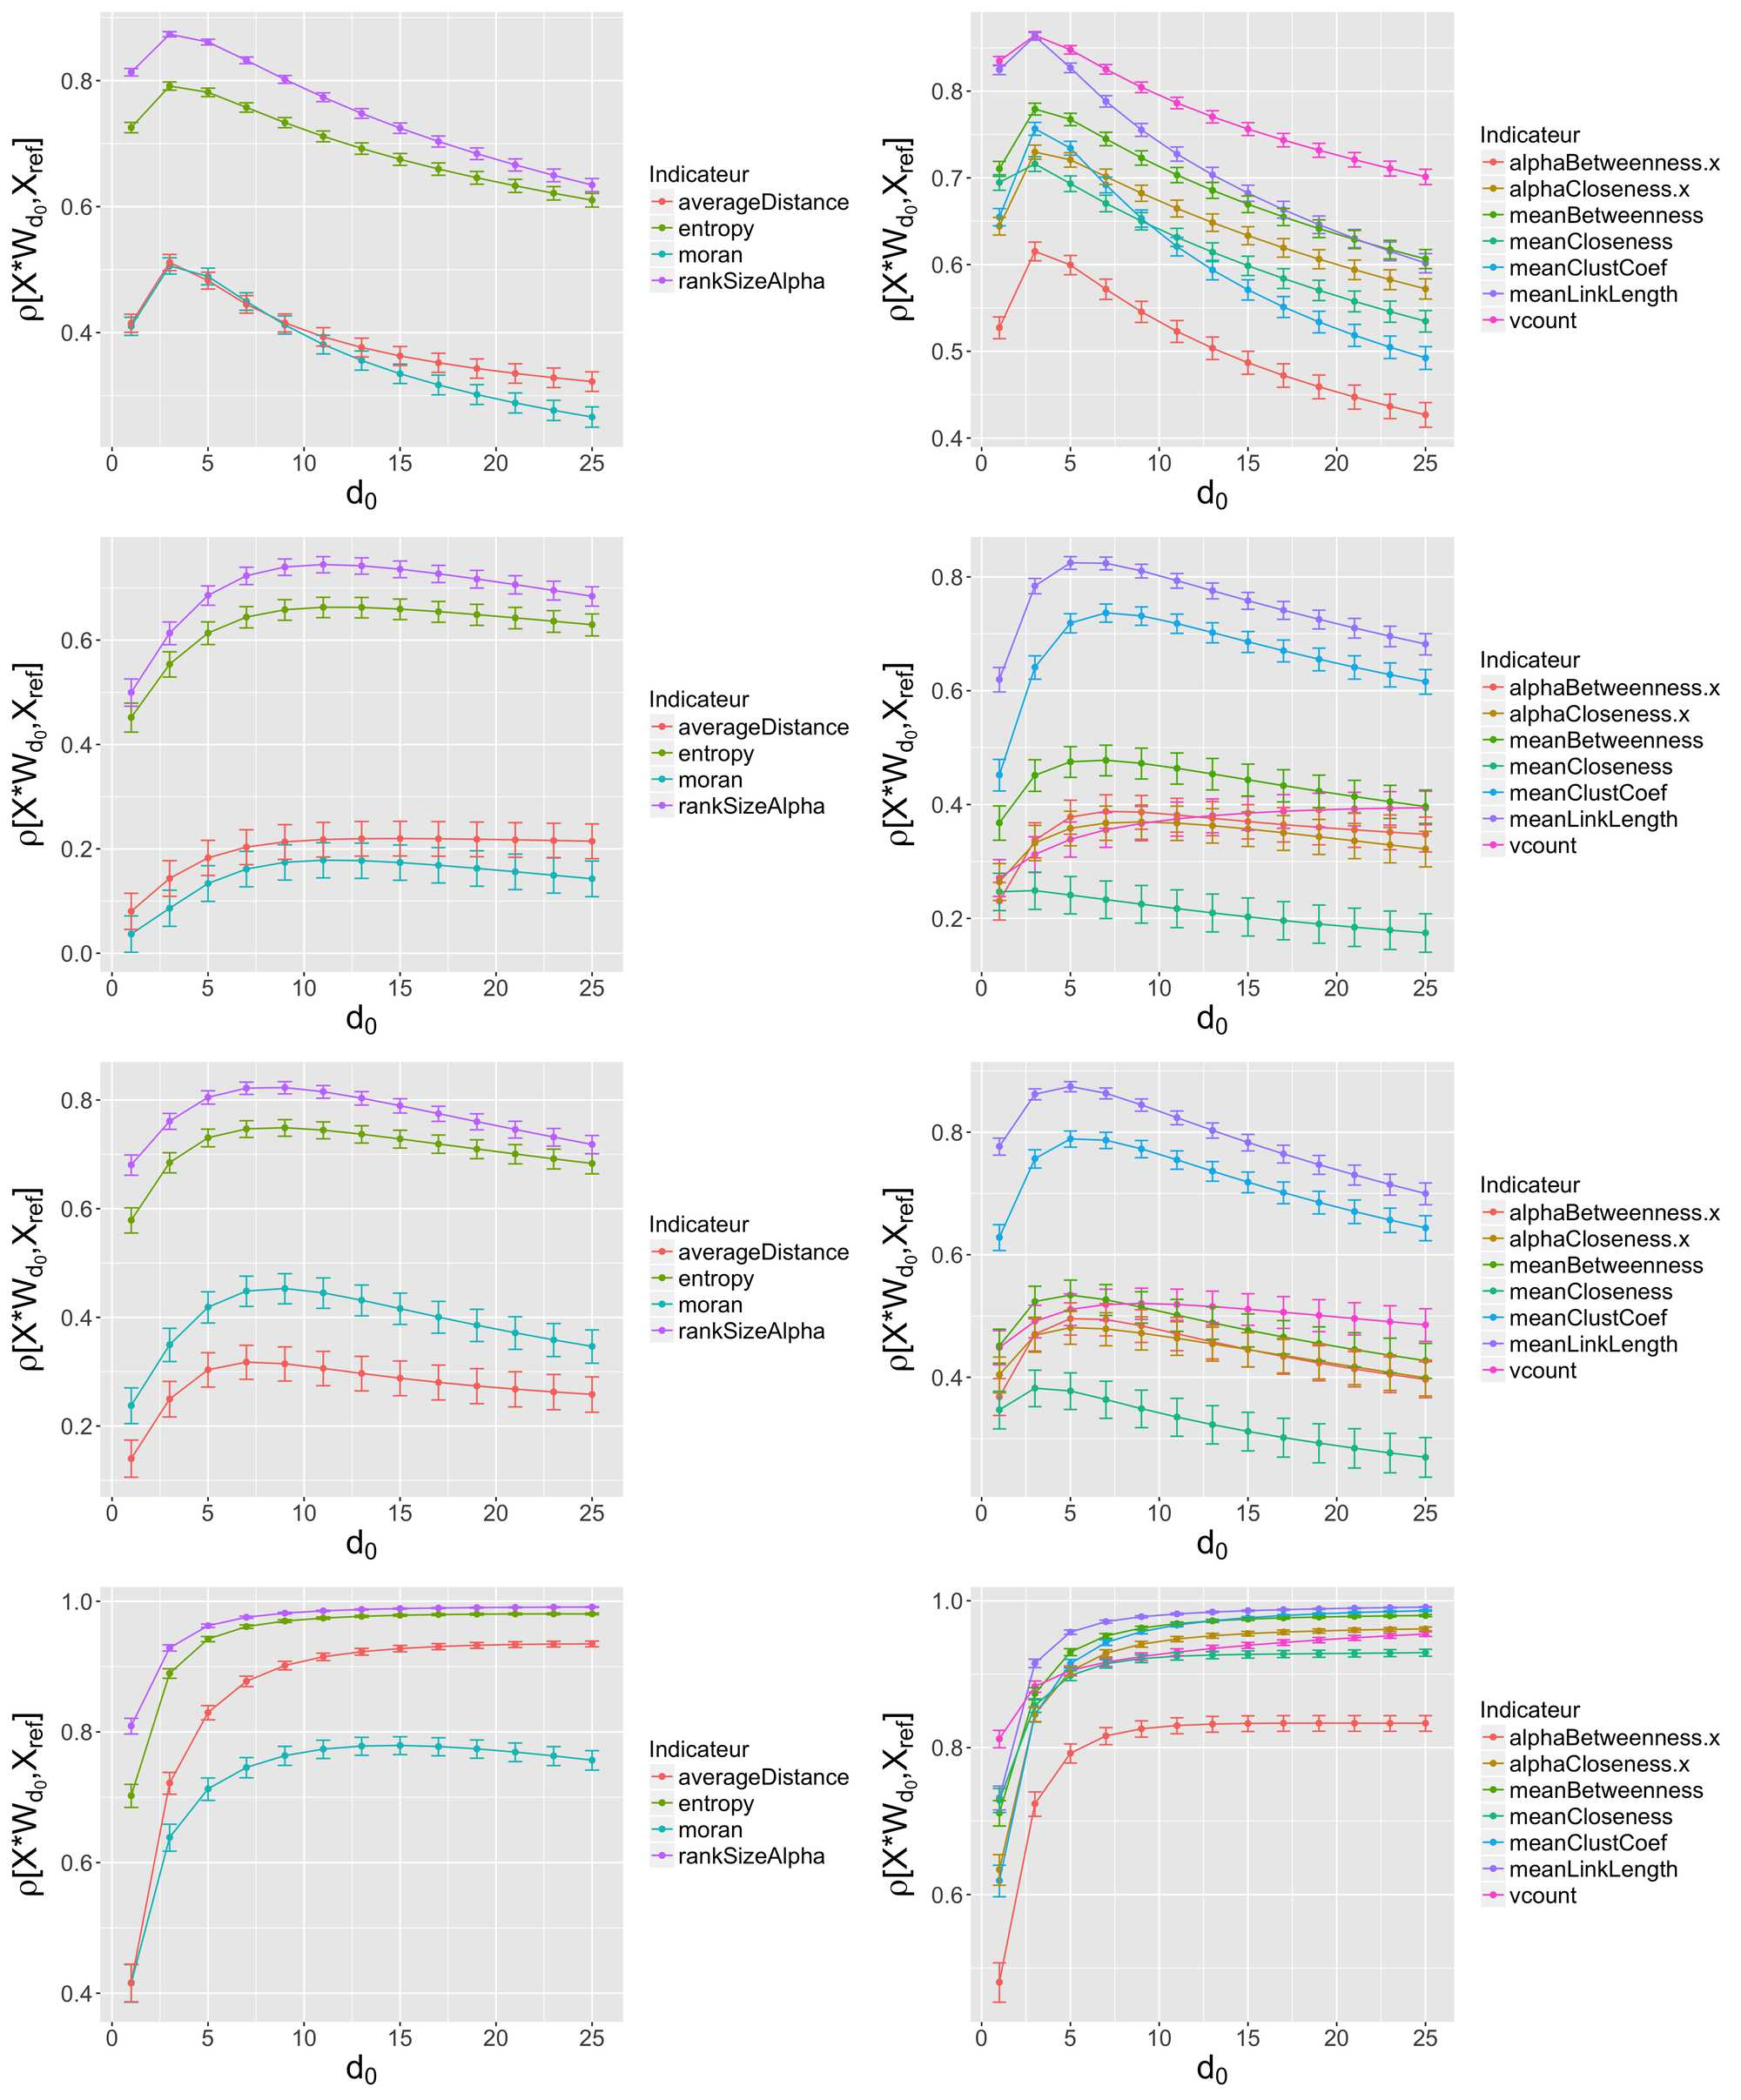
\includegraphics[width=\linewidth,height=0.9\textheight]{Figures/Final/A-staticcorrelations-sensitivity-corrs.jpg}
	\appcaption{\label{fig:app:staticcorrelations:sensitivity-corrs}}{\textbf{Corrélations entre indicateurs à différentes échelles.} \label{fig:app:staticcorrelations:sensitivity-corrs}}
\end{figure}
%%%%%%%%%%%%












\subsection{Spatial Correlations}{Corrélations Spatiales}

La Fig.~\ref{fig:app:staticcorrelations:europe_correlations} donne la distribution spatiale pour l'ensemble de l'Europe, d'un échantillon de corrélations entre indicateurs : $\rhob{\alpha_{cl}}{I}$, $\rhob{\gamma}{\alpha}$, $\rhob{\bar{bw}}{\gamma}$.

%%%%%%%%%%%%%%
\begin{figure}
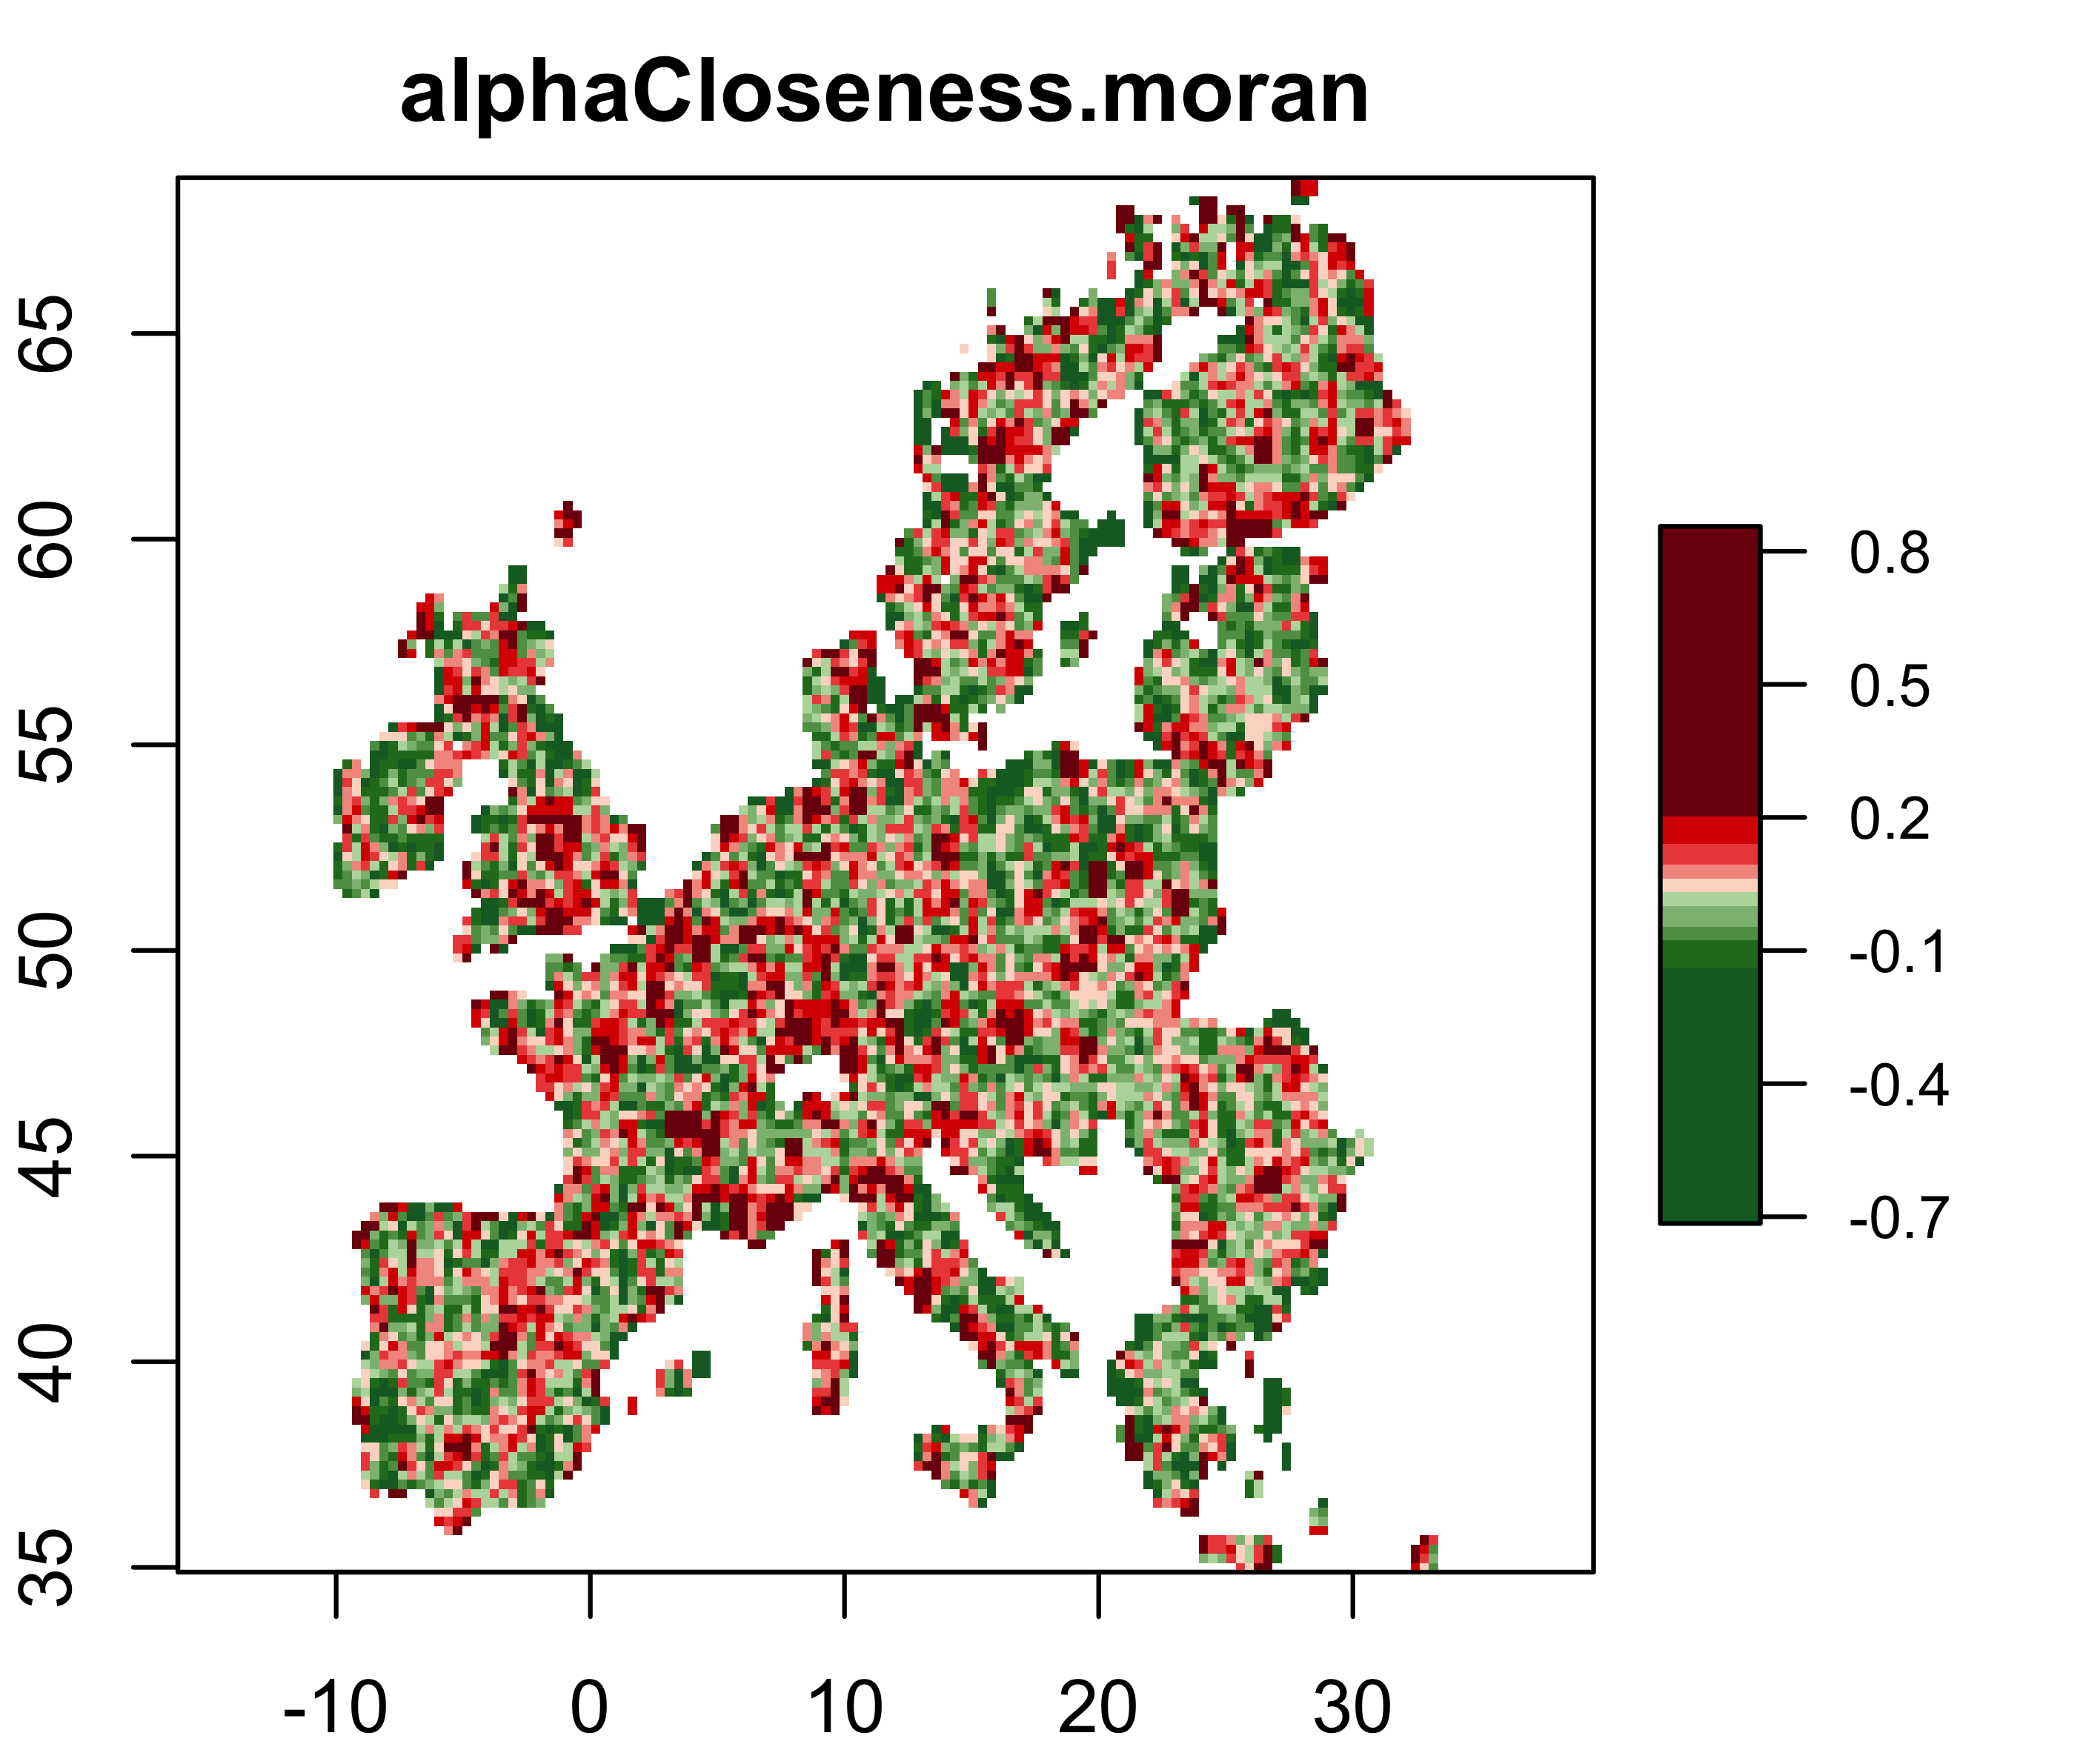
\includegraphics[width=0.48\linewidth]{Figures/StaticCorrelations/EU_corr_alphaCloseness_moran_rhoasize12}
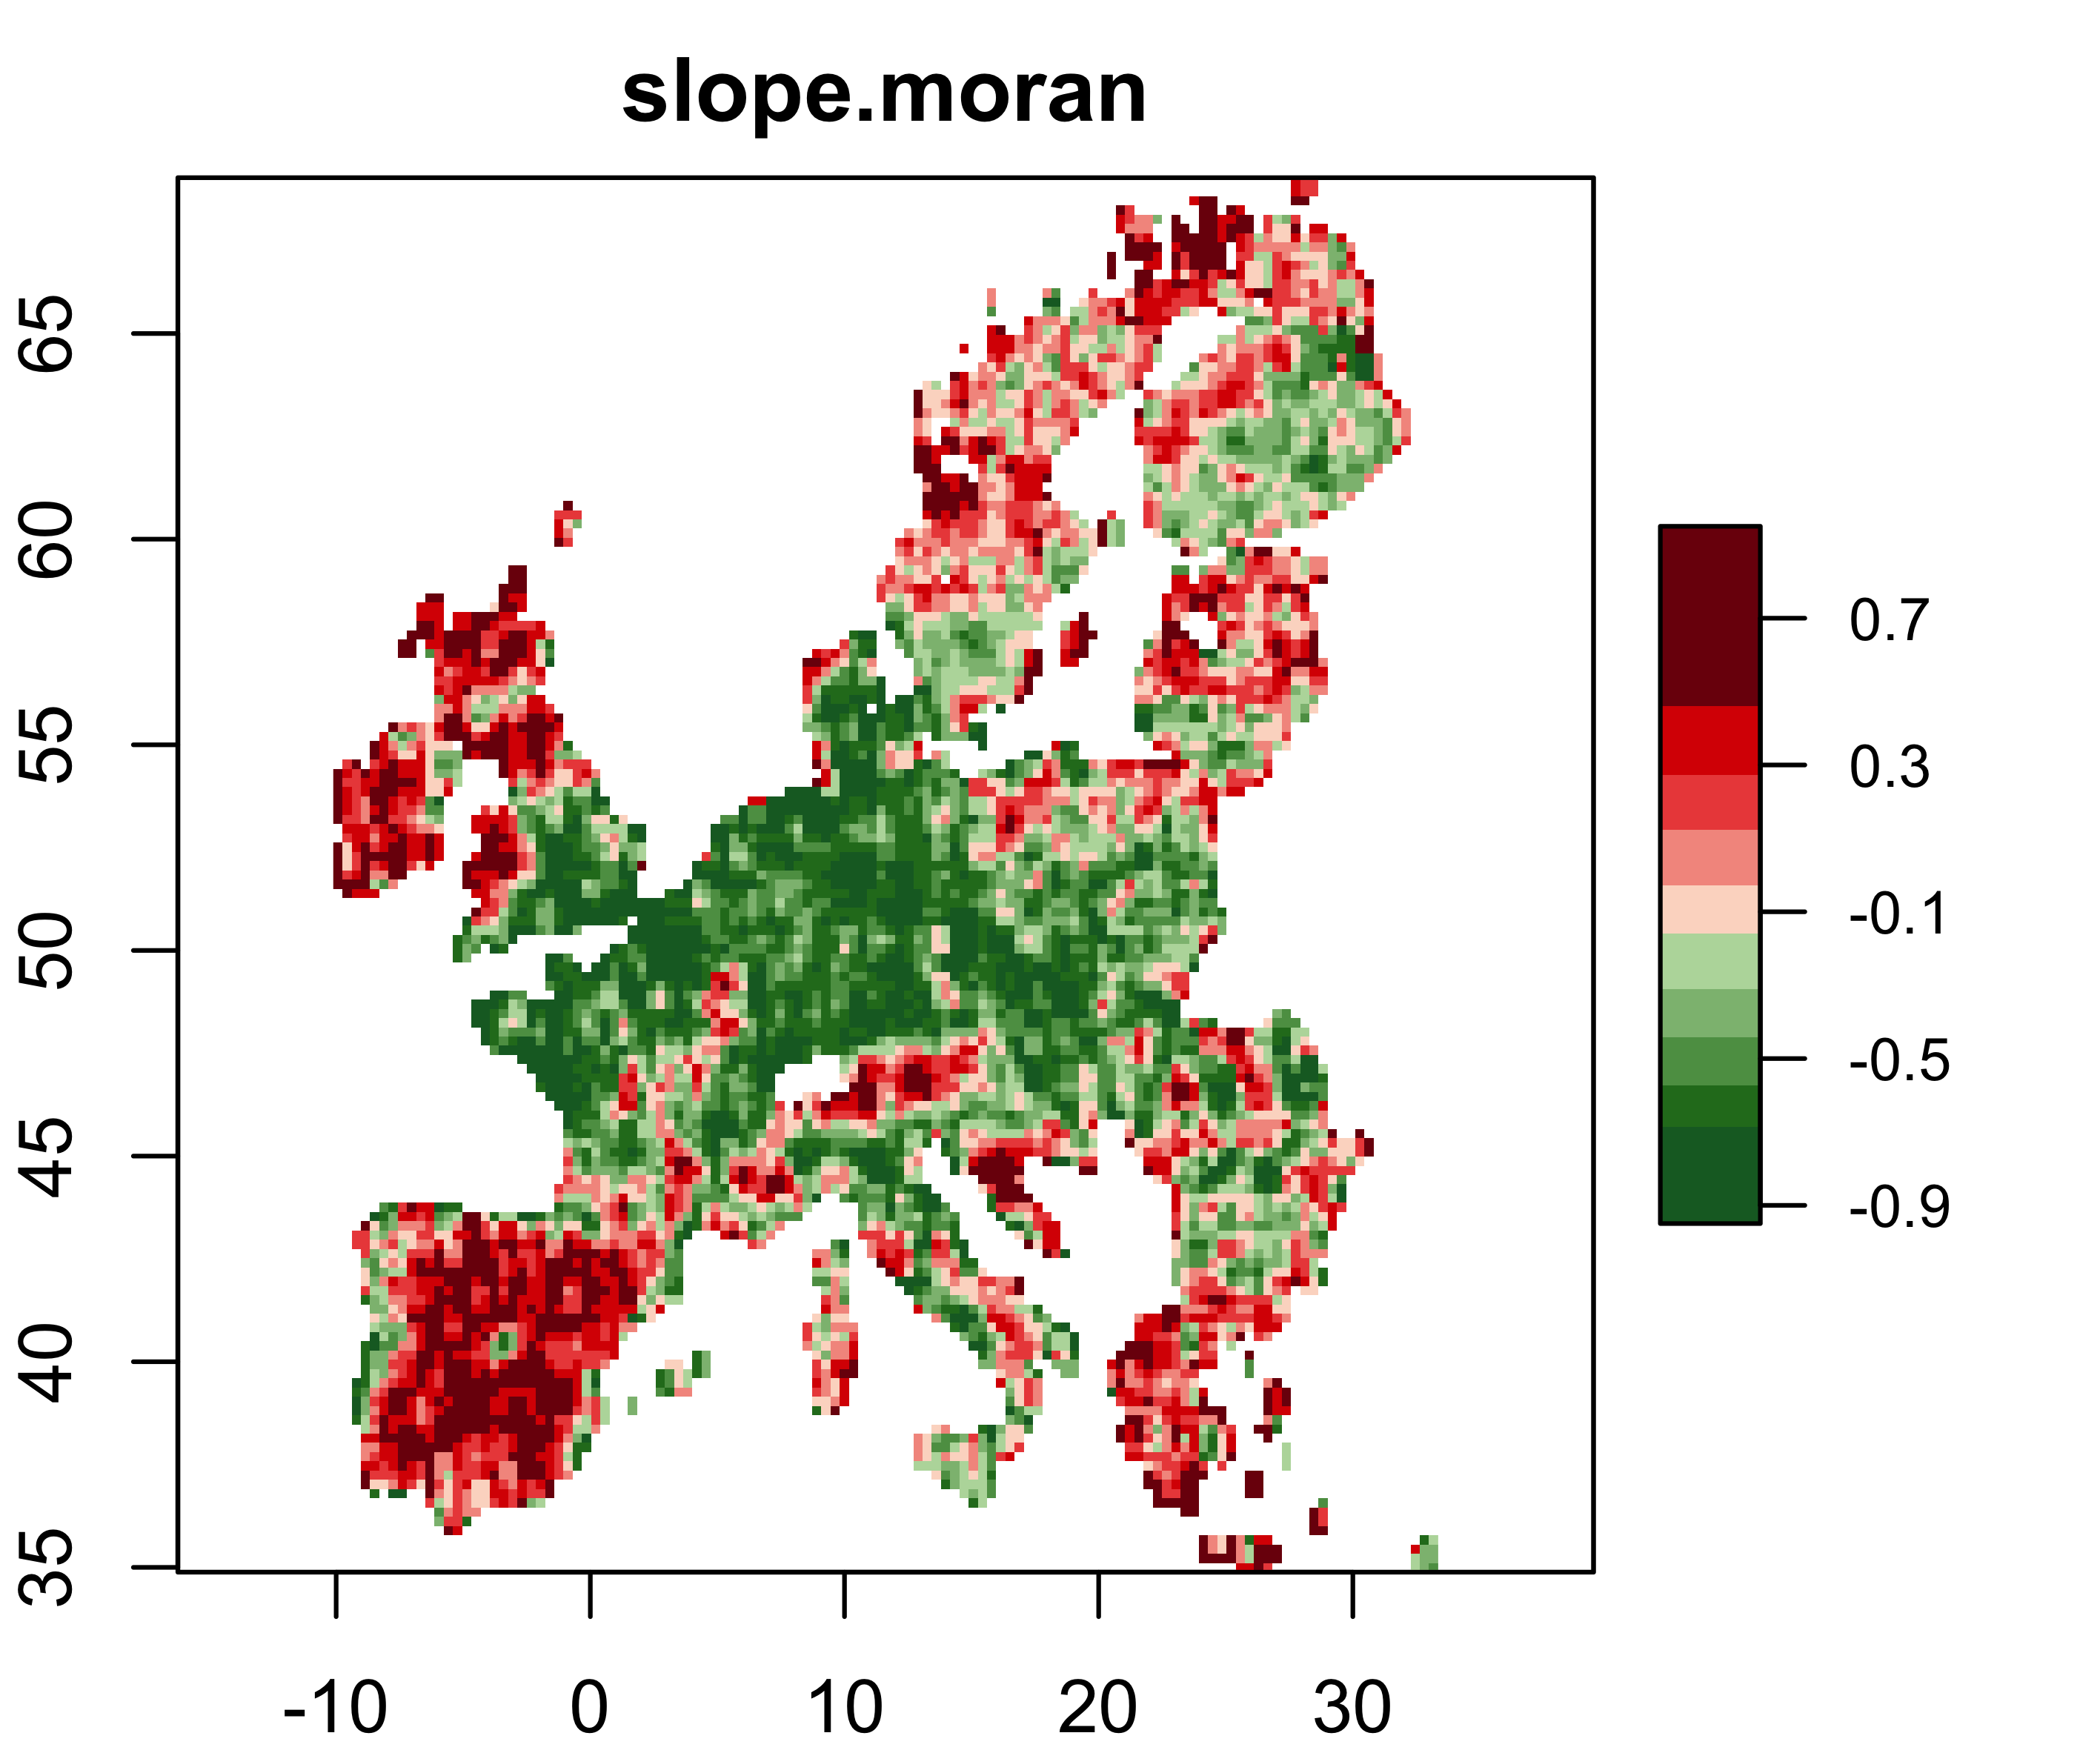
\includegraphics[width=0.48\linewidth]{Figures/StaticCorrelations/EU_corr_slope_moran_rhoasize12}\\
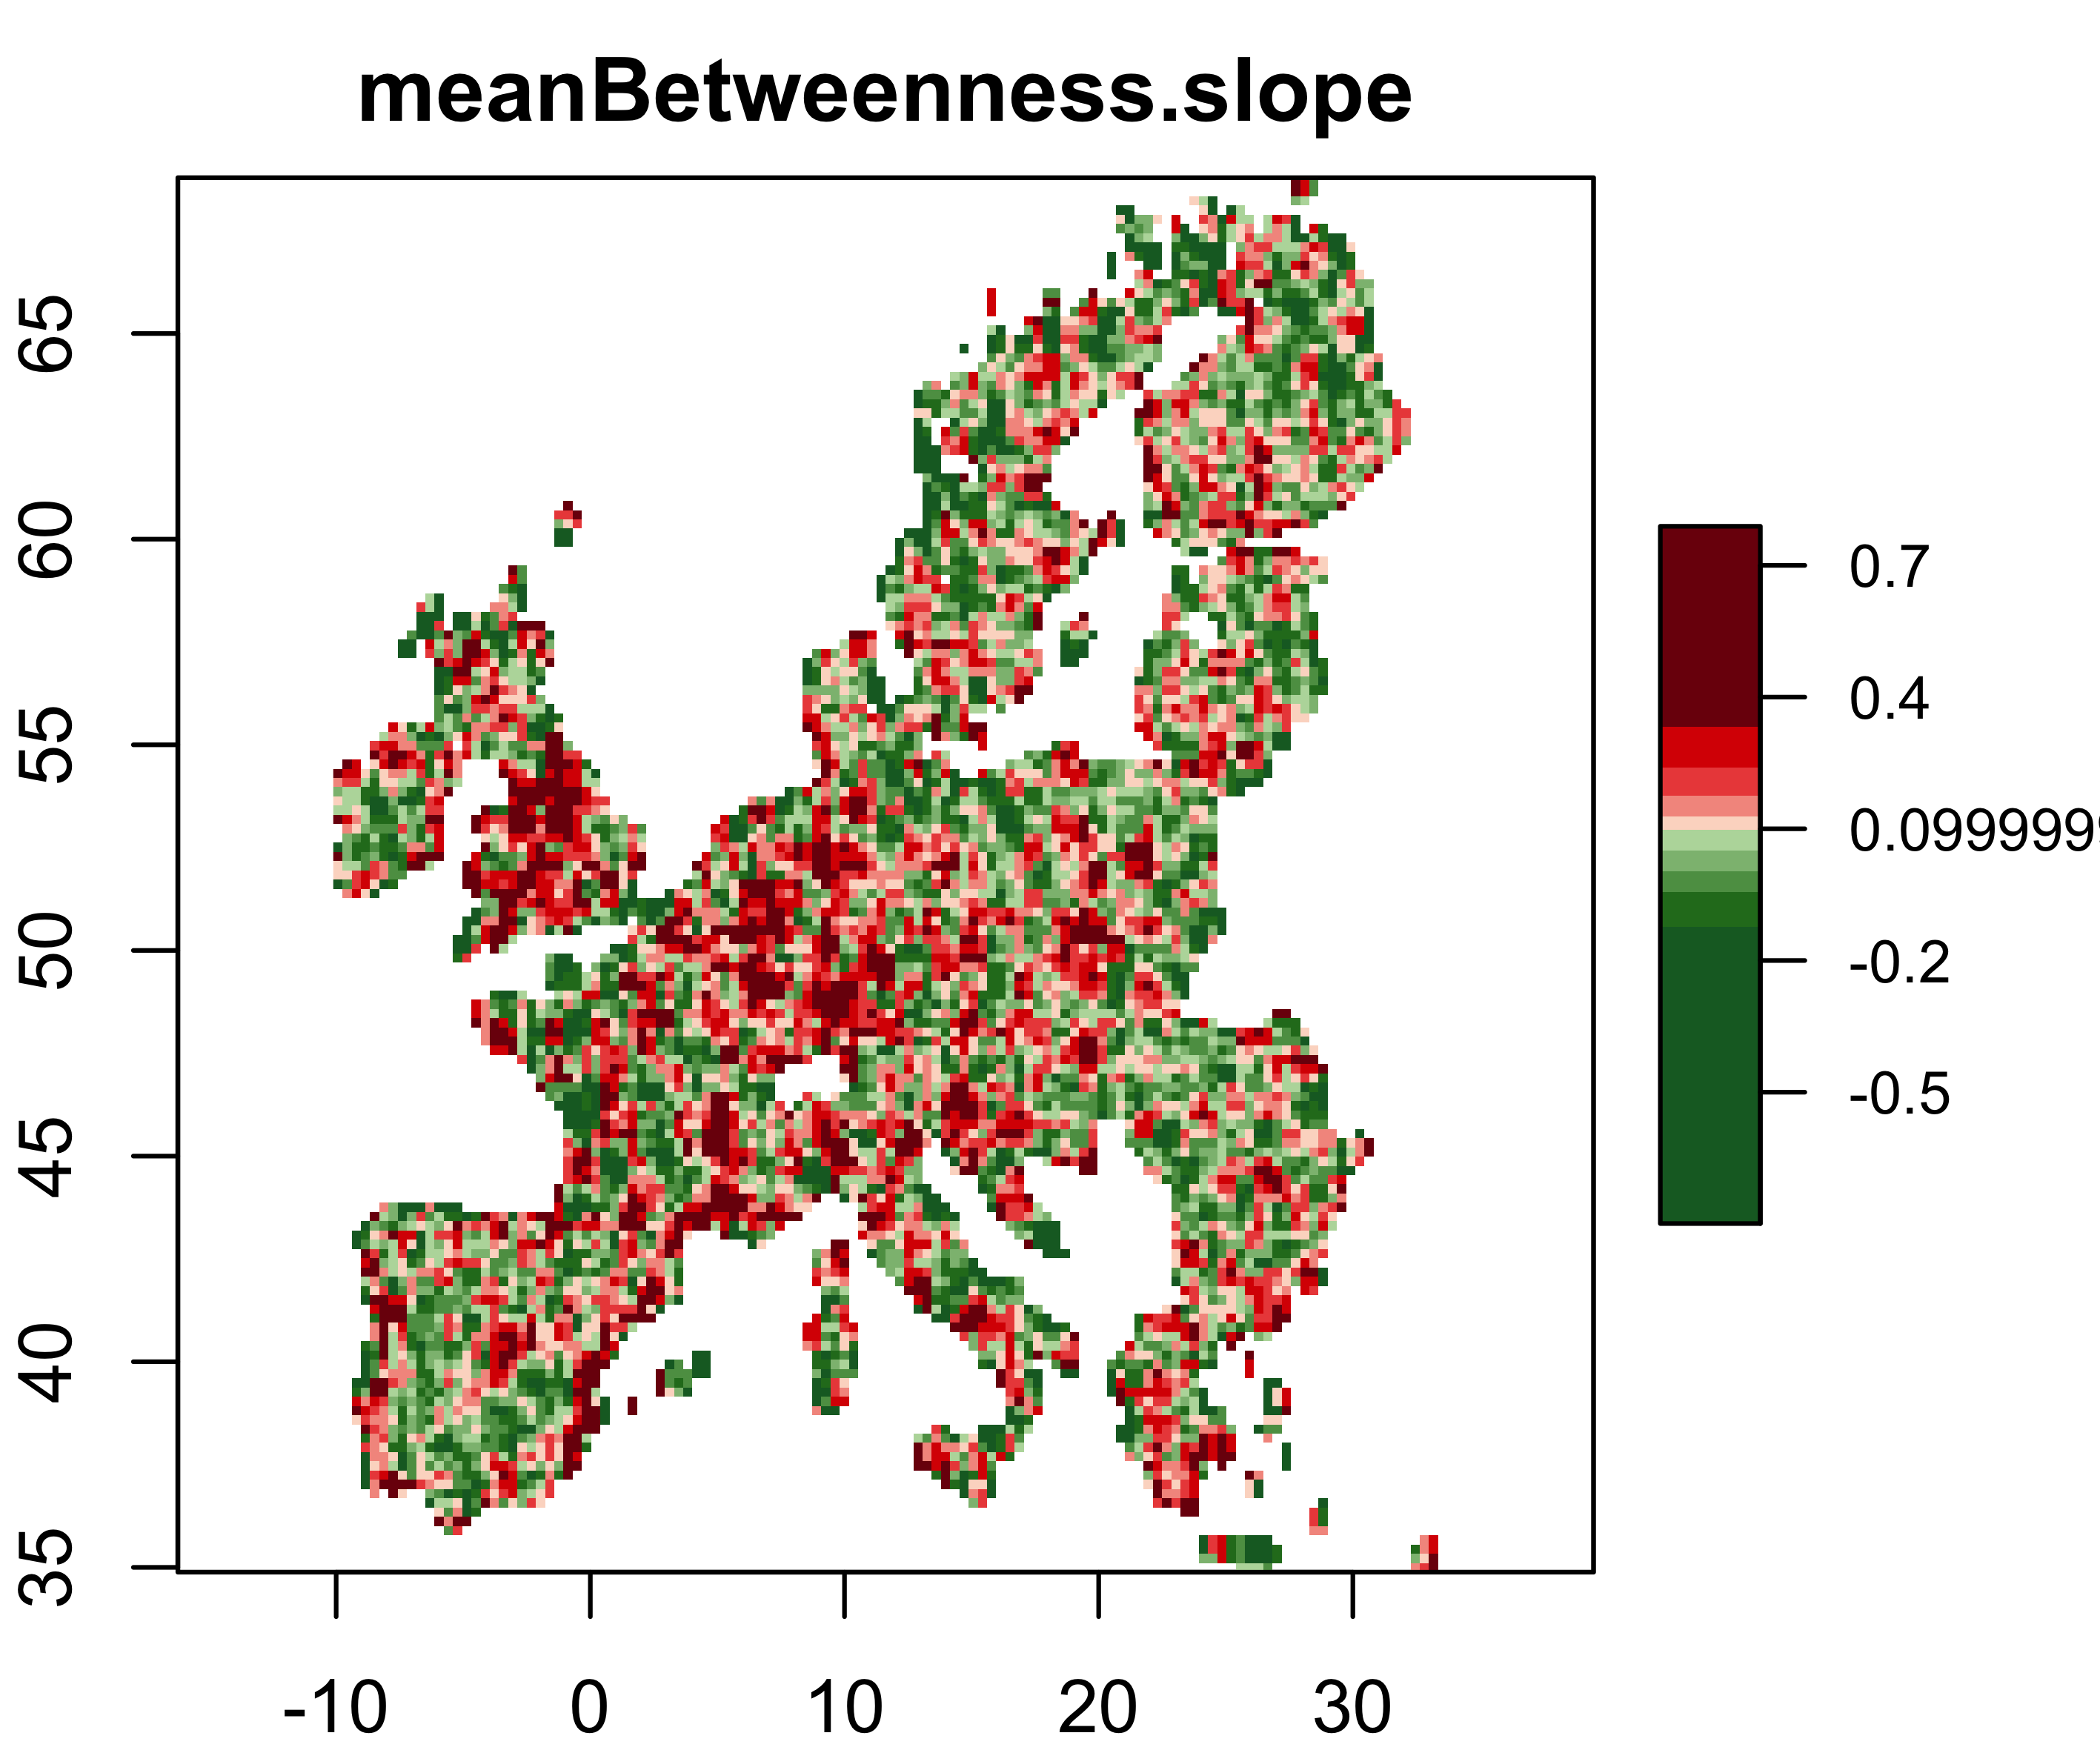
\includegraphics[width=0.48\linewidth]{Figures/StaticCorrelations/EU_corr_meanBetweenness_slope_rhoasize12}
\appcaption{}{\textbf{Correlations spatiales pour l'Europe.}\label{fig:app:staticcorrelations:europe_correlations}}
\end{figure}
%%%%%%%%%%%%%%



La Fig.~\ref{fig:app:staticcorrelations:corr-distribs} donne les distributions statistiques des correlations estimées, pour différentes valeurs de $\delta$.


%%%%%%%%%%%%%%
\begin{figure}
%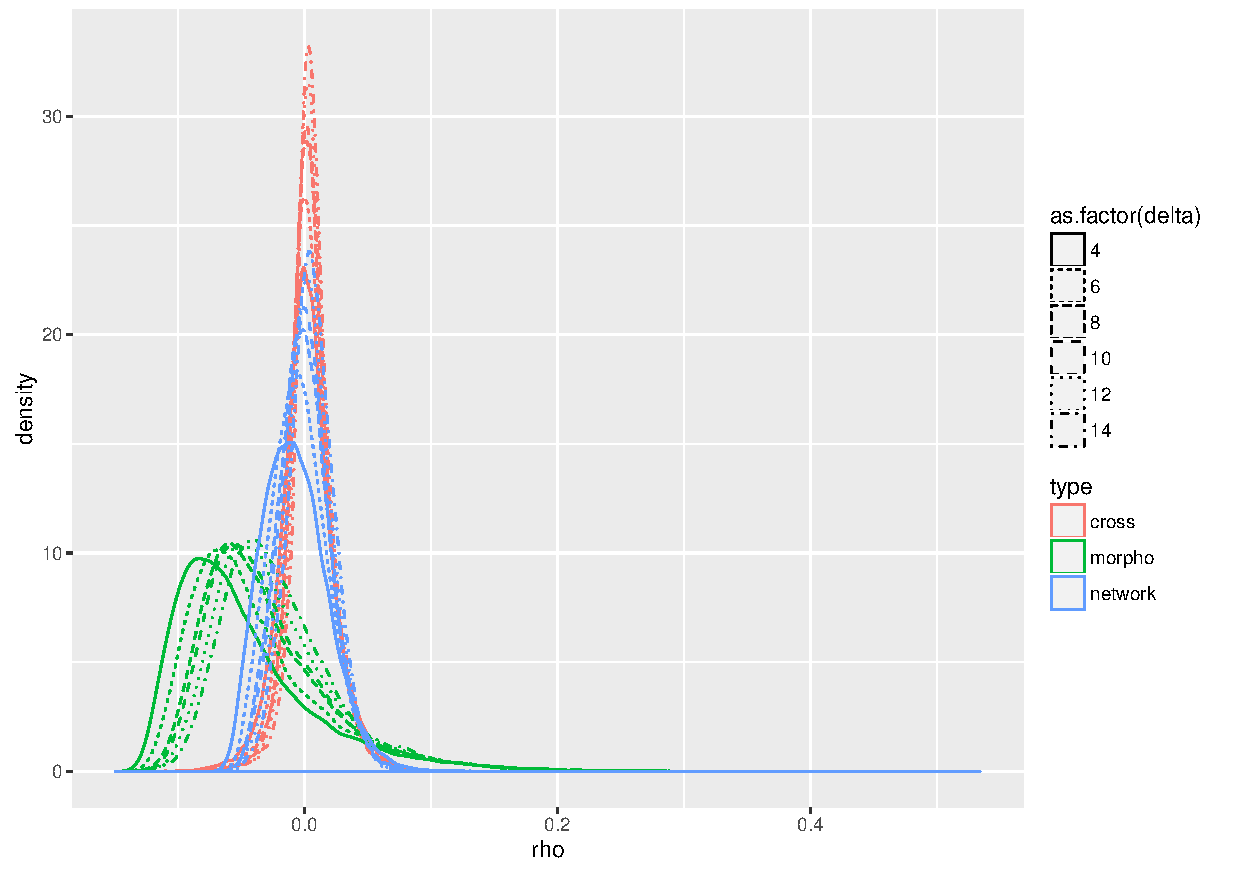
\includegraphics[width=0.48\linewidth]{Figures/StaticCorrelations/corrs-distrib_varyingdelta_bytype}
%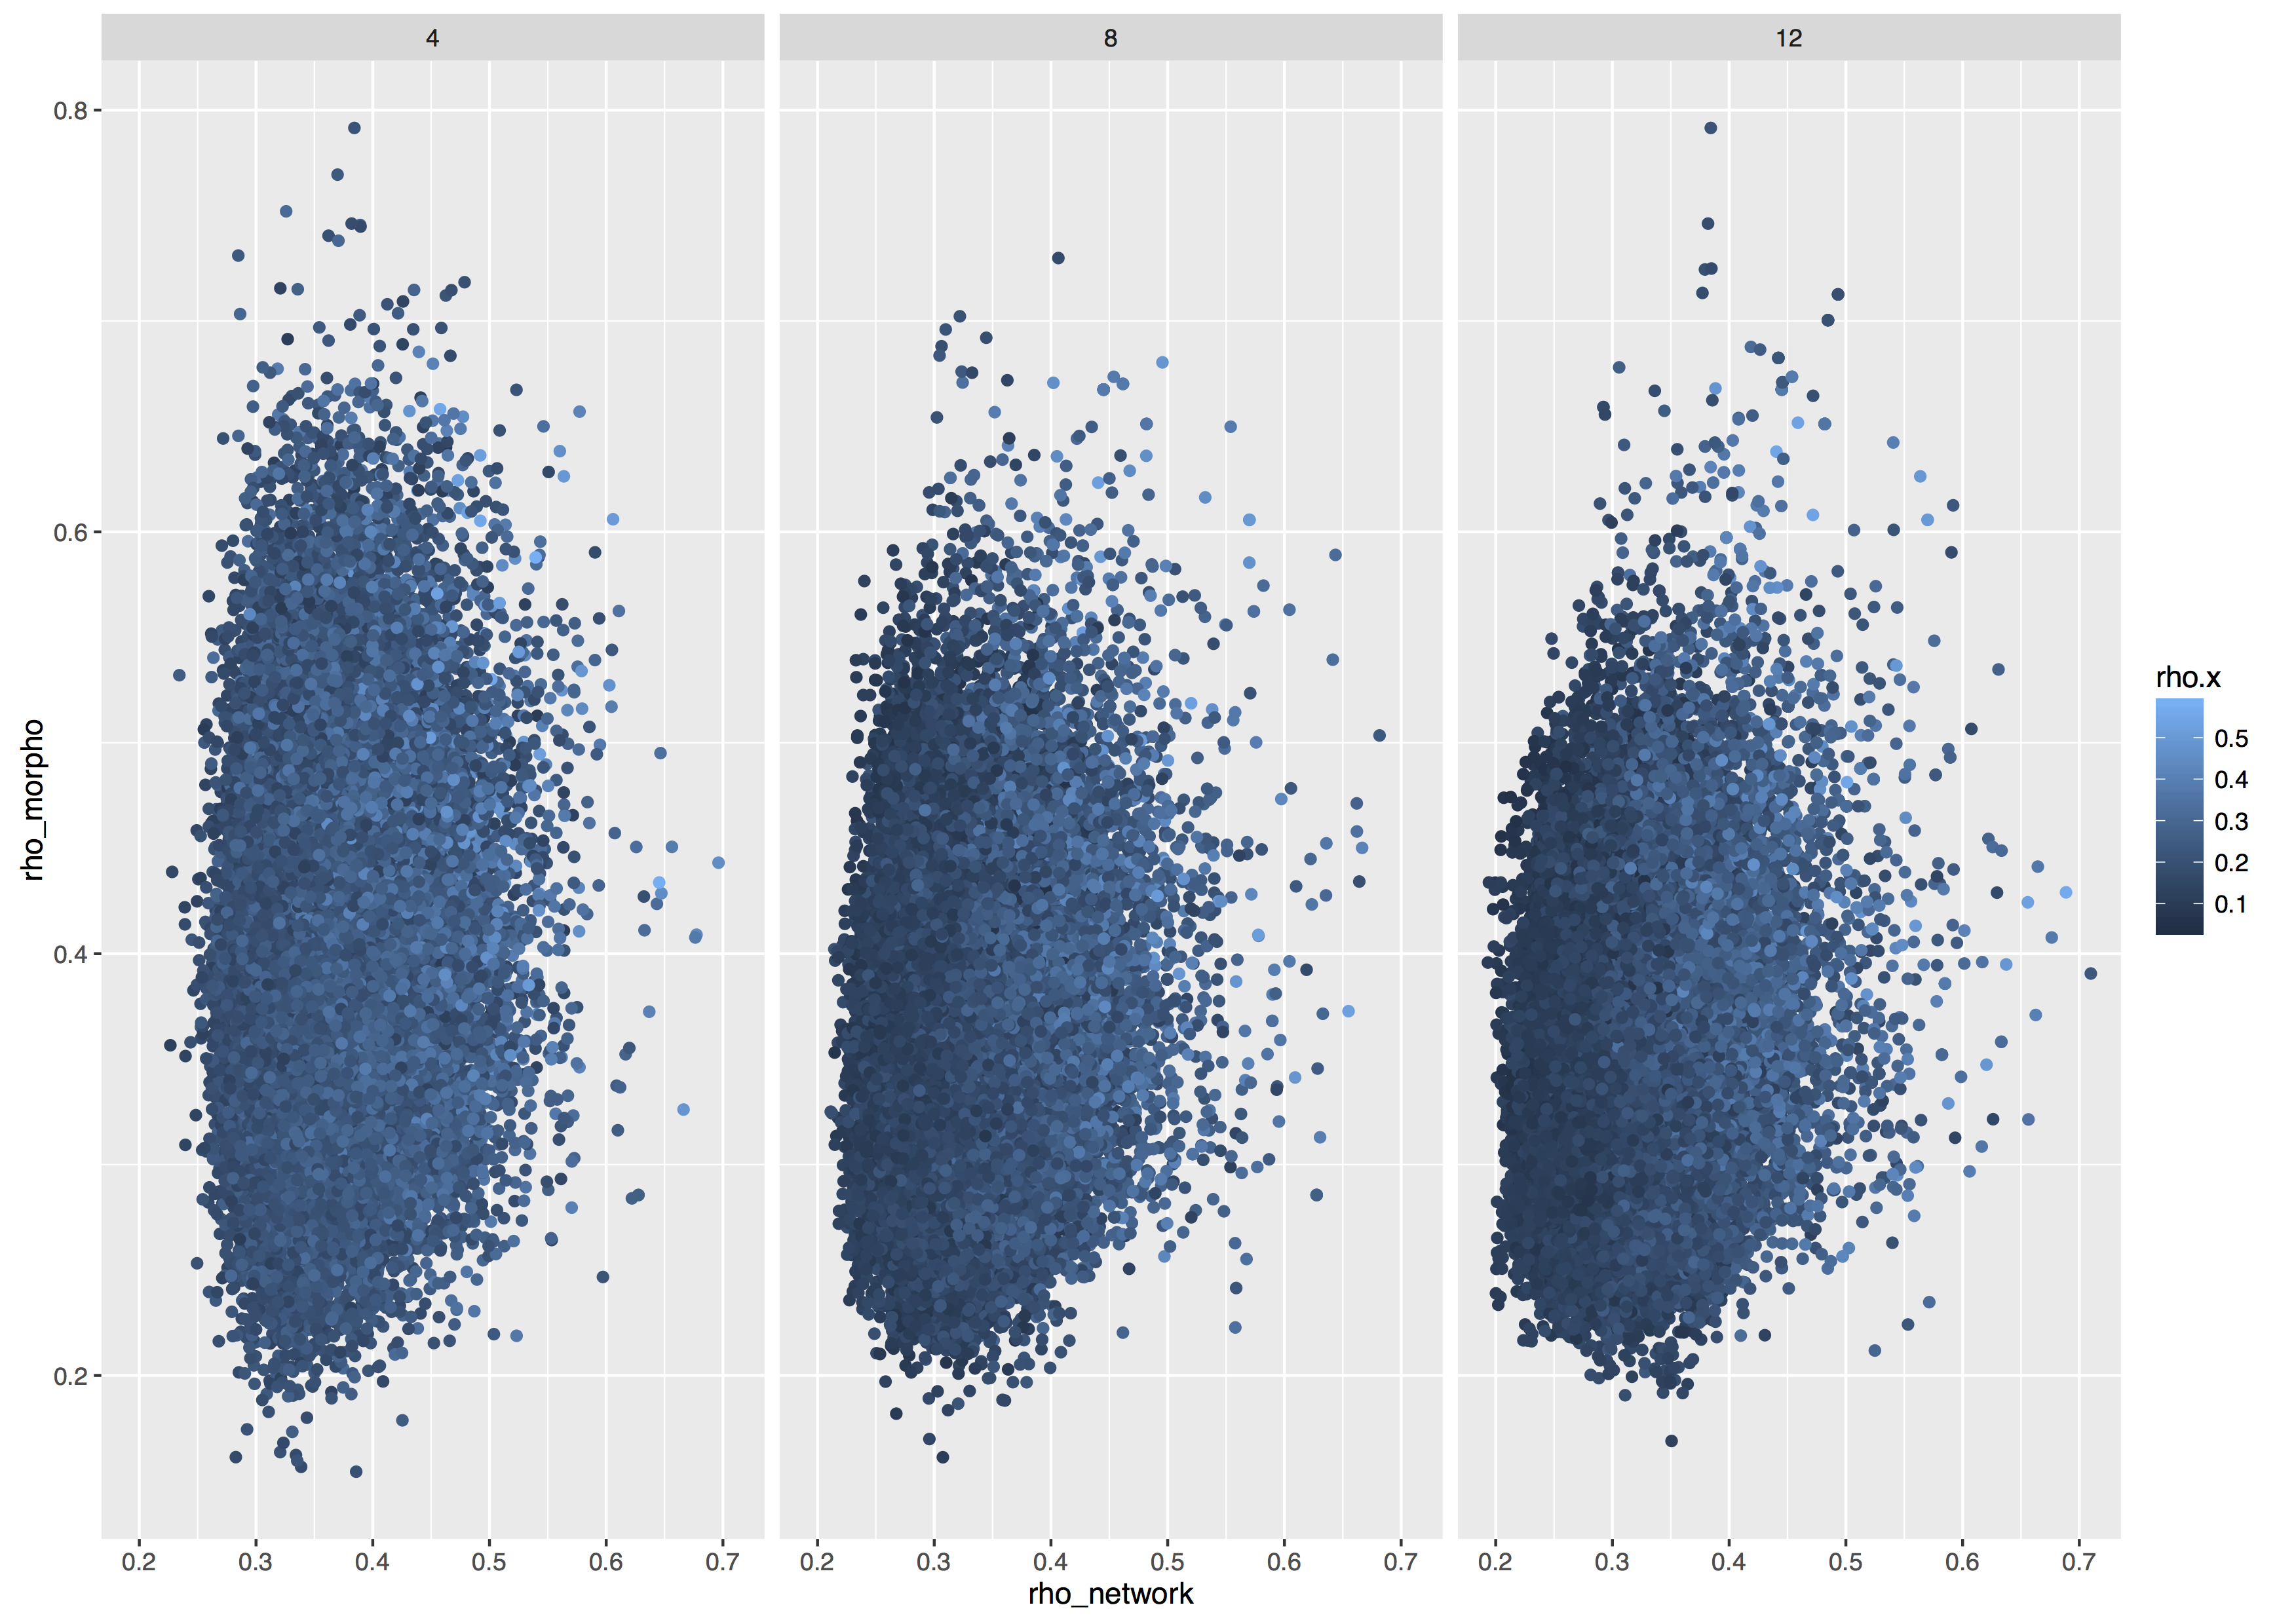
\includegraphics[width=0.48\linewidth]{Figures/StaticCorrelations/scatter_meanabs_colcross}
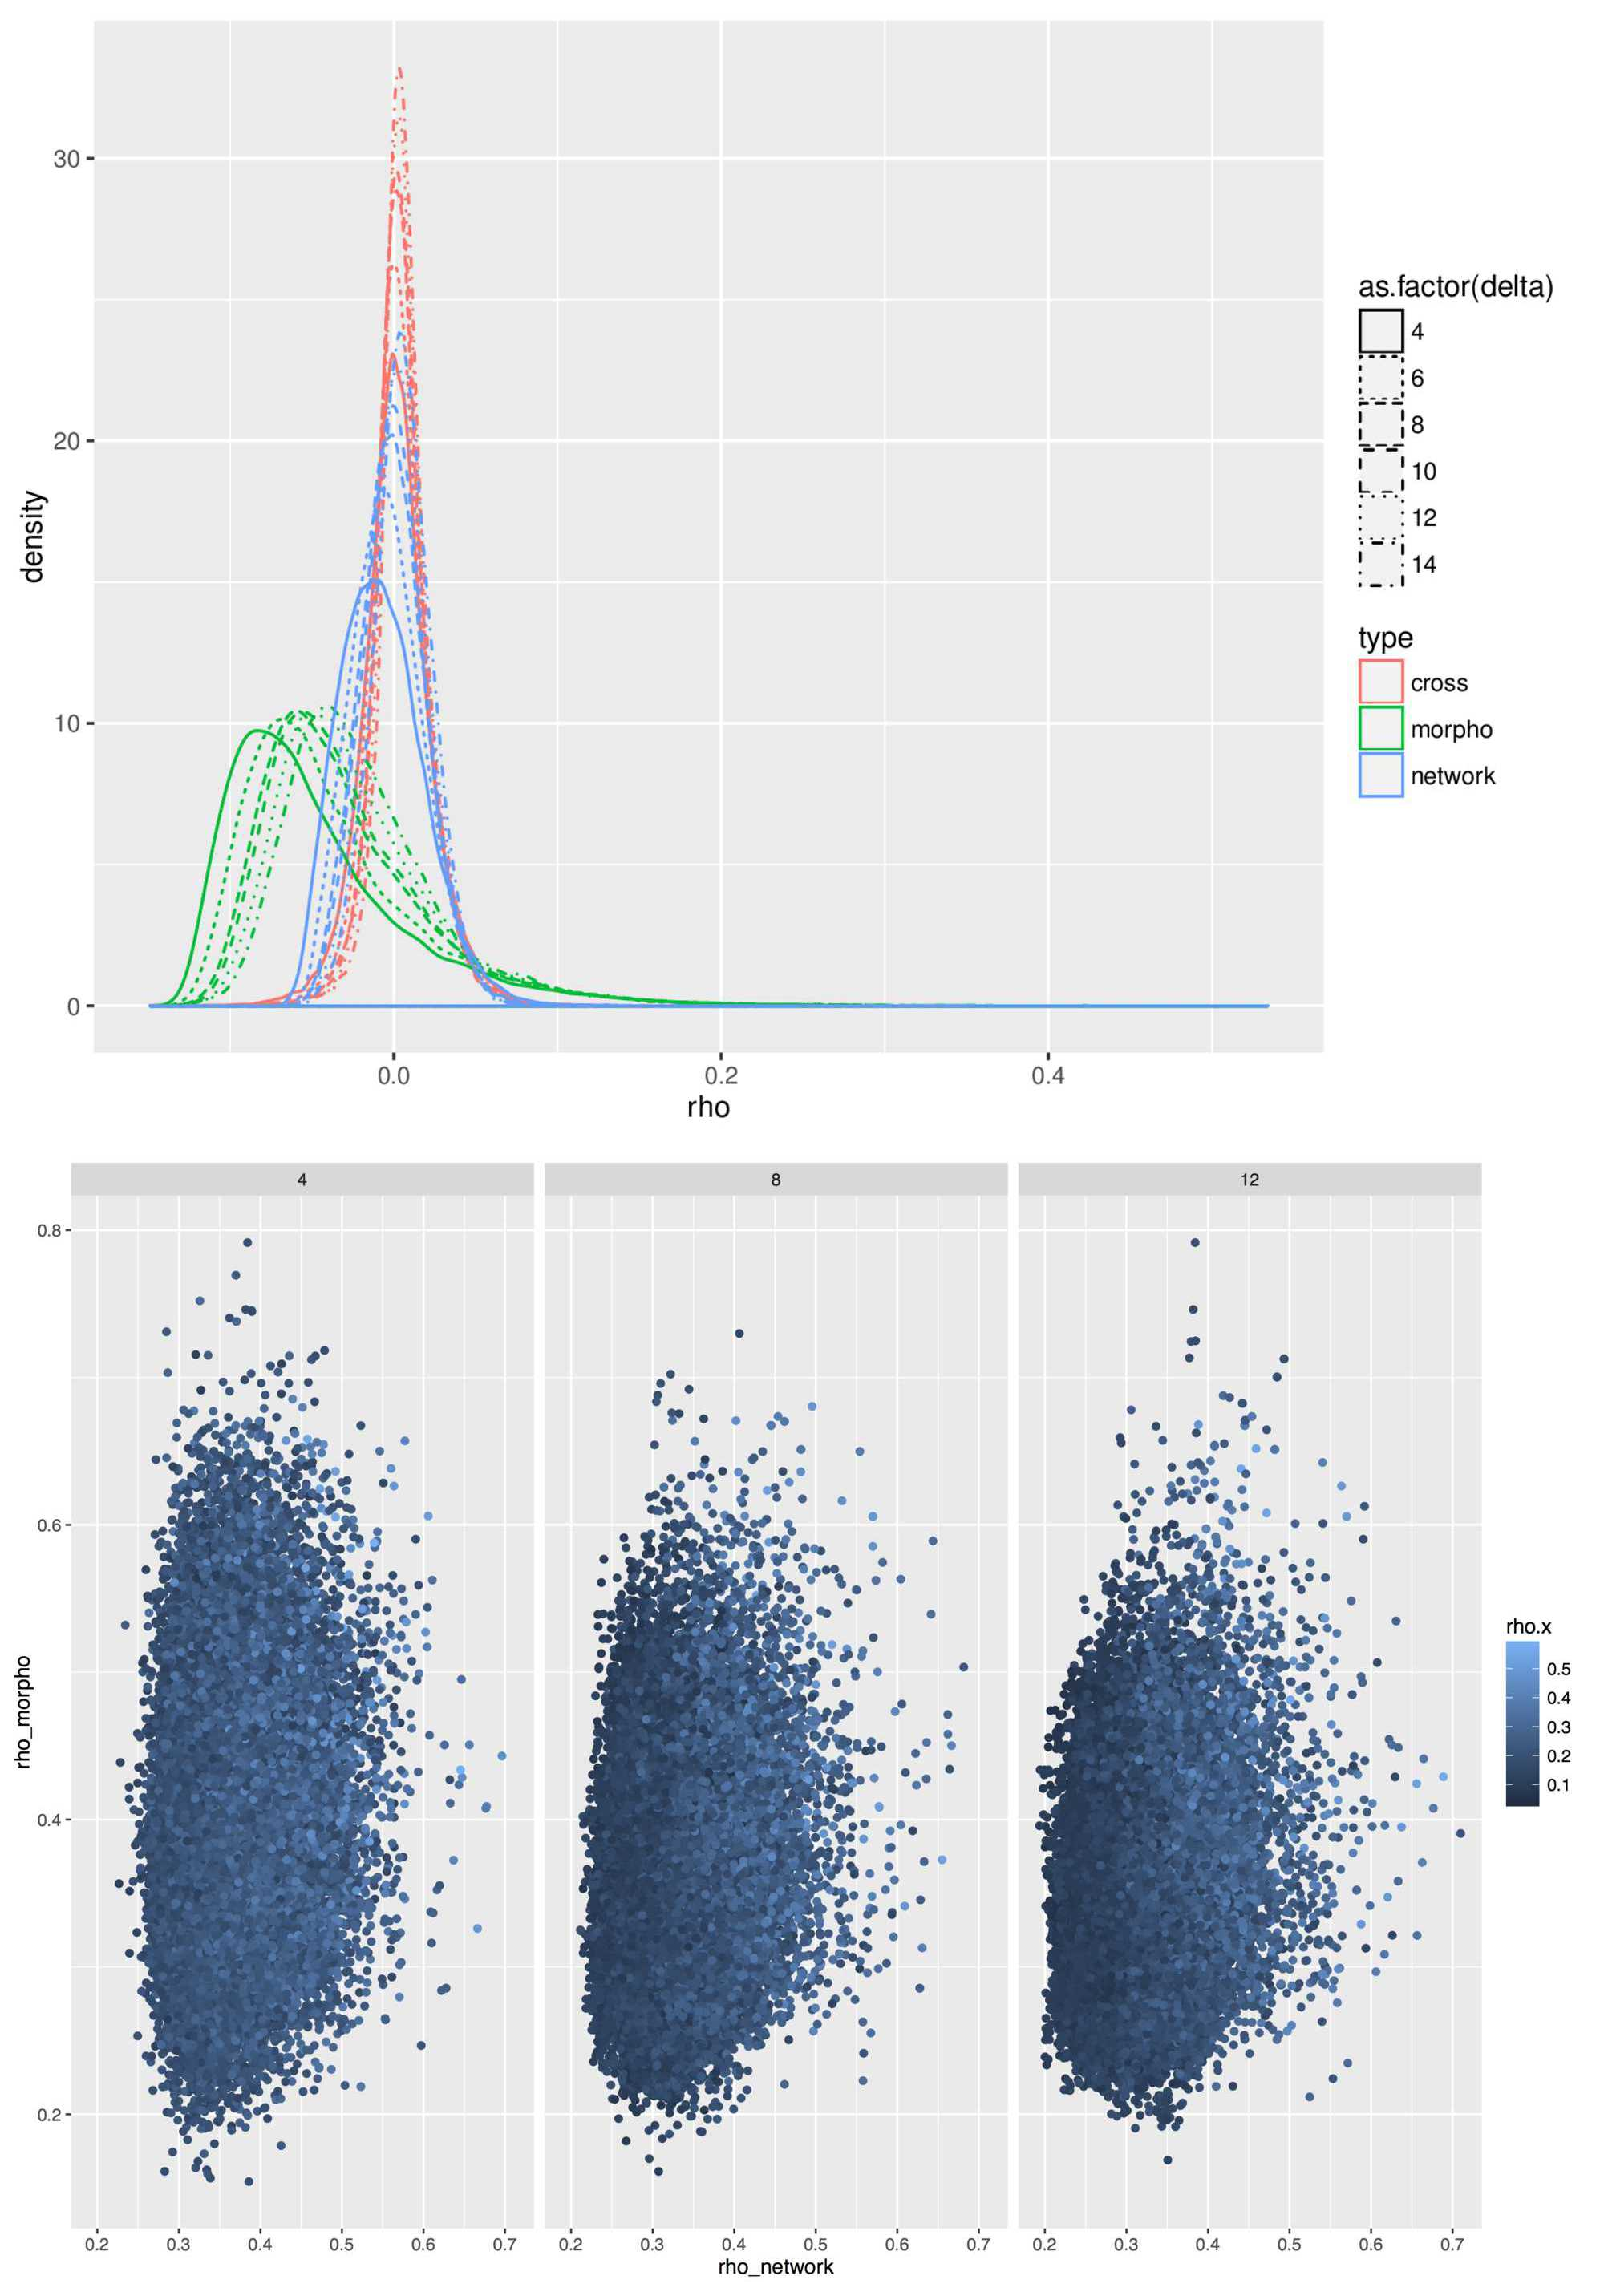
\includegraphics[width=\linewidth,height=0.9\textheight]{Figures/Final/A-staticcorrelations-corr-distribs.jpg}
\appcaption{}{\textbf{Distribution des corrélations.} \textit{(Haut Gauche)} Distribution statistique des corrélations, pour les différents blocs morphologiques, réseau et corrélations croisées (couleur), pour différentes valeurs de $\delta$ (type de ligne) ; \textit{(Bas Droite)} Correlation absolues moyennes pour le réseau en fonction de la morphologie, niveau de couleur donnant la corrélation croisée, pour différentes valeur de $\delta$.\label{fig:app:staticcorrelations:corr-distribs}}
\end{figure}
%%%%%%%%%%%%%%


%%%%%%%%%%%%%%
%% -- ON HOLD --

%%%%%%%%%%%%%%
%\begin{figure}
%
%\caption[][]{}{Correlations spatiales pour la Chine.}
%\label{fig:app:staticcorrelations:morphocn}
%\end{figure}
%%%%%%%%%%%%%%




%%%%%%%%%%%%%%
\subsection{Multi-scale}{Multi-scalarité}


\subsubsection{Estimation of correlations for a multi-scalar process}{Estimation des corrélations pour un processus multi-scalaire}

Nous proposons ici de relier le caractère multi-scalaire d'un processus stochastique spatio-temporel avec l'estimation de sa matrice de correlation. Pour simplifier et dans le cadre où ce résultat est utilisé en texte principal, nous considérons des corrélations statiques estimées dans l'espace. Pour simplifier également, considérons des processus ayant deux échelles caractéristiques se superposant linéairement, c'est à dire s'écrivant sous la forme
\[
X_i = X_i^{(0)} + \tilde{X}_i
\]
avec $X_i^{(0)}$ tendance aux petites échelles ayant une distance caractéristique d'évolution $d_0$, et $\tilde{X}_i$ signal évoluant à une distance caractéristique $d \ll d_0$.

Nous pouvons alors calculer la décomposition de la corrélation entre deux processus, de manière similaire à ce qui est fait en~\ref{app:sec:syntheticdata-finance}. En supposant que $\Covb{X_i^{(0)}}{\tilde{X}_j}$ pour tous $i,j$, et en notant $\varepsilon_i = \frac{\sigma\left[X_i^{(0)}\right]}{\sigma\left[\tilde{X}_i\right]}$ le rapport des écarts type entre tendance et signal, il y a
\[
\begin{split}
	\rho\left[X_1,X_2\right] & = \rho\left[X_1^{(0)} + \tilde{X}_1,X_2^{(0)} + \tilde{X}_2\right]\\
	& = \frac{\Covb{\tilde{X}_1}{\tilde{X}_2} + \Covb{X_1^{(0)}}{X_2^{(0)}}}{\sqrt{\left(\Varb{X_1^{(0)}} + \Varb{\tilde{X}_1}\right)\left(\Varb{X_2^{(0)}} + \Varb{\tilde{X}_2}\right)}}\\
	& = \frac{\varepsilon_1 \varepsilon_2\rho\left[X_1^{(0)},X_2^{(0)}\right] + \rho\left[\tilde{X}_1,\tilde{X}_2\right]}{\sqrt{\left(1 + \varepsilon_1^2\right)\left(1 + \varepsilon_2^2\right)}}
\end{split}
\]

En supposant $\varepsilon_i \ll 1$, on peut développer cette expression au premier ordre et obtenir

\begin{equation}
	\rho\left[X_1,X_2\right] = \left( \varepsilon_1 \varepsilon_2\rho\left[X_1^{(0)},X_2^{(0)}\right] + \rho\left[\tilde{X}_1,\tilde{X}_2\right]\right)\cdot\left(1 - \frac{1}{2}(\varepsilon_1^2 + \varepsilon_2^2)\right)
\end{equation}

L'ajout de la tendance au signal introduit ainsi une correction sur la corrélation, d'une part par la prise en compte directe de la corrélation entre tendance atténuée, et d'autre part par le terme d'interférence en facteur.

Pour appliquer ce résultat à notre problématique, supposons que $d \simeq l_0$,$l_0$ étant la distance minimale d'estimation des corrélations. On a par ailleurs l'échelle de stationnarité $d_s$ qui correspond à l'échelle de variation des corrélations, et selon les résultats empiriques vérifie $d_s > l_0$, significativement au moins pour certains indicateurs (par exemple hiérarchie et Moran, pour laquelle elle est de l'ordre du pays). Enfin, notons $\delta_0 = d_0/d$ l'échelle de la tendance en termes de $\delta$. On suppose donc

\[
d < d_s < d
\]

Pour les valeurs de $\delta$ telles que $\delta \cdot d < d_s$, on devrait avoir $\hat{\Cov}_{\delta}\left[\tilde{X}_1,\tilde{X}_2\right] \simeq \hat{\Cov}_{\delta = 1}\left[\tilde{X}_1,\tilde{X}_2\right]$ si $\hat{\Cov}_{\delta}$ est l'estimateur sur la zone de taille $\delta$.

Par ailleurs, on peut supposer raisonnablement que $\hat{\Var}_{\delta = 1}\left[X_i^{(0)}\right] \ll \hat{\Var}_{\delta = d_s / d}\left[X_i^{(0)}\right]$, c'est à dire que la tendance est constante à la plus petite échelle en comparaison des variations aux échelles intermédiaires.

Sous ces hypothèses, l'estimateur de $\rho$ devrait varier en fonction de $\delta$ selon les variations de $\varepsilon_i$ en fonction de $\delta$. En supposant enfin les tendances très peu corrélées (effets structurels indépendants), on conserve la correction d'interférence dans l'expression de $\rho$, et donc que $\rho(\delta)$ décroit pour des faibles valeurs de $\delta$.


Nous avons ainsi démontré qu'une structure simple multi-scalaire du processus implique une variation de la corrélation estimée en fonction de $\delta$, sous un certain nombre d'hypothèse. La réciproque n'a a priori pas de raison d'être vraie. Le lien que nous opérons ici est ainsi une illustration pour renforcer une hypothèse, qui est par ailleurs également soutenue par les résultats sur la variation de l'intervalle de confiance décrits par la suite.



\subsubsection{Confidence interval for correlation}{Intervalle de confiance pour la corrélation}

Nous dérivons ici le comportement de l'estimateur de corrélation en fonction de la taille de l'échantillon. Sous l'hypothèse de distribution normale de deux variables aléatoire $X,Y$, alors la transformée de Fisher de l'estimateur de Pearson $\hat{\rho}$ telle que $\hat{\rho} = \tanh (\hat{z})$ a une distribution normale. Si $z$ est la transformée de la corrélation réelle $\rho$, alors un intervalle de confiance pour $\rho$ est de taille

\[
\rho_{+} - \rho_{-} = \tanh (z + k / \sqrt{N}) - \tanh (z - k / \sqrt{N})
\]

où $k$ est une constante. Comme $\tanh{z} = \frac{\exp (2z) - 1}{\exp (2z) + 1}$, on peut développer puis réduire cette expression, pour obtenir

\[
\begin{split}
	\rho_{+} - \rho_{-} & = 2\cdot \frac{\exp (2k/\sqrt{N})-\exp (-2k/\sqrt{N})}{\exp (2z)-\exp (-2z) + \exp (2k/\sqrt{N}) + \exp (-2k/\sqrt{N})}\\
	& = 2\cdot \frac{\sinh{(2k/\sqrt{N})}}{\cosh{(2z)} + \cosh{(2k/\sqrt{N})}}
\end{split}
\]

En utilisant le fait que $\cosh u \sim_0 1 + u^2/2$ et que $\sinh u \sim_0 u$, on obtient bien que $\rho_{+} - \rho_{-} \sim_{N\gg 0} k' / \sqrt{N}$.\qed





%%%%%%%
%% -- ON HOLD --
% ergod spatio-temporelle


%\bpar{
%Analytical Deductions
%1. \textbf{Regimes of temporal correlations.} Let assume local ergodicity in $\vec{x}_0$ at scale $\delta \cdot l_0$ (reasonable with urban growth and network extension in recent times). The Ergodic theorem implies that $\exists \mathcal{T}$ such that
%
%\[<Y_i (t) >_{\norm{\vec{x}-\vec{x}_0} < \delta\cdot l_0} = <Y_i (\vec{x}_0)>_{t\in \mathcal{T}}\] 
%
%With spatial stationarity, $<Y_i>_{\vec{x}_0}=<Y_i>_{\vec{x}_1}$, thus $\mathcal{T}$ must be constant to be invariant by translation. By contraposition and (2), processes have different dynamical characteristics.
%% if translate in a given direction, looses a small part, must be compensated by the area translated by delta (overlap), thus must be constant.
%}{
%Nous suggérons que la non-stationnarité spatiale est reliée d'une part à différentes échelles de temps impliquées, et d'autre part à une non-ergodicité globale\comment[FL]{le lecteur ne te suit plus : c'est trop rapide}, sous l'hypothèse de stationnarité et d'ergodicité locale.
%
% Supposons ergodicité locale en $\vec{x}_0$ à l'échelle $\delta \cdot l_0$ à laquelle nous estimons les corrélations. Alors le théorème ergodique fournit un échantillonnage temporel $\mathcal{T}$ tel que 
%\[
%<Y_i (t) >_{\norm{\vec{x}-\vec{x}_0} < \delta\cdot l_0} = <Y_i (\vec{x}_0)>_{t\in \mathcal{T}}
%\]
%\comment[FL]{c'est du raisonnement de matheux, ca n'est pas comprehensible dans ce contexte}
%En se plaçant en un autre point $\vec{x}_1$ assez loin\comment[FL]{?}, la stationnarité spatiale devrait impliquer $<Y_i>_{\vec{x}_0}=<Y_i>_{\vec{x}_1}$ et $\mathcal{T}$ sera similaire pour garder invariance par translation. Par contraposition comme on a montré la non-stationnarité, les processus ont ainsi nécessairement des caractéristiques dynamiques différentes.
%
%}



%%%%%%%%%%%%%%
%\begin{figure}
%\begin{mdframed}
%	Montrons que la non-stationnarité spatiale implique des caractéristiques dynamiques différentes, au sens que $\frac{\partial Y}{\partial t}(x_0,t) \neq \frac{\partial Y}{\partial t}(x_1,t)$ pour tous $t$ et $x_0,x_1$ tels que $\norm{x_0 - x_1} \gg \delta $.
%
%	\medskip
%\noun{Encadré : } \textit{Non-stationnarité spatiale et non-ergodicité}
%\end{mdframed}
%\end{figure}
%%%%%%%%%%%%%%

%\bpar{
%2. \textbf{Global non-ergodicity.} Let $X_k$ a partition of space into local areas. We have $<\cdot>_x = \sum_k w_k <\cdot>_{x_k} =_{(1)} \sum_k w_k <\cdot>_{\mathcal{T}_k} $. On the other hand, global ergodicity would give $<\cdot>_t = <\cdot>_{\mathcal{T}} = \sum_k w_k <\cdot>_{\mathcal{T}}$ and $\sum_k w_k \left(<\cdot>_{\mathcal{T}} - <\cdot>_{\mathcal{T}_k}\right) = 0$. Being true on each subset implies $\mathcal{T}=\mathcal{T}_k$, what contradicts (1).
%}{
%Concernant la non-ergodicité globale, soit $X_k$ une partition de l'espace en zones locales. On a  $<\cdot>_x = \sum_k w_k <\cdot>_{x_k} = \sum_k w_k <\cdot>_{\mathcal{T}_k} $. Mais d'autre part, l'ergodicité globale impliquerait que  $<\cdot>_t = <\cdot>_{\mathcal{T}} = \sum_k w_k <\cdot>_{\mathcal{T}}$ et donc $\sum_k w_k \left(<\cdot>_{\mathcal{T}} - <\cdot>_{\mathcal{T}_k}\right) = 0$.\comment[FL]{notations non comprehensibles} Pour que cette relation soit vraie sur la totalité des sous-ensembles, il est nécessaire que $\mathcal{T}=\mathcal{T}_k$, ce qui contredit la propriété montrée précédemment, et le système global est nécessairement non-ergodique. Ces résultats dépendent des hypothèses théoriques, mais nous postulons qu'ils devraient rester vrais de manière empirique vu les suggestions\comment[FL]{???} de la Théorie Evolutive. \comment[FL]{je ne suis pas certain que ton raisonnement soit entierement valide. il faut en discuter car ta demonstration ecrite n'est pas assez claire pour que je puisse en juger.}
%}

















\stars





%----------------------------------------------------------------------------------------

\newpage


%%%%%%%%%%%%%%%%%%%%%%%
\section{Causality regimes}{Régimes de causalité}

\label{app:sec:causalityregimes}




%%%%%%%%%%
%% -- Digressions : not useful --

%\subsubsection{Context Formalization}{Formalisation}

%\subsubsection{Variables}

%\paragraph{Description}

%We assume a dynamic transportation network $n(\vec{x},t)$ within a dynamic territorial landscape $\vec{T}(\vec{x},t)$, which components are to simplify population $p(\vec{x},t)$ and employments $e(\vec{x},t)$. Data is structured the following way :
%\begin{itemize}
%\item Observation of territorial variables are discretized in space and in time, i.e. the spatial field $\vec{T}$ is summarized by $\mathbf{T} = \left(\vec{T}(\vec{x}_i,t_j^{(T)})\right)_{i,j}$ with $1\leq i \leq N$ and $1\leq j \leq T$. They concretely correspond to census on administrative units (\emph{communes} in our case) at different dates.
%\item Network has a continuous spatial position but is represented by the vector of network distances $\mathbf{N}$ \comment{(Florent) vol d'oiseau/distance temps ? second faisable et à privilégier je pense}
%\end{itemize}

%\paragraph{Definitions}

%\subsubsection{On Accessibility}{Sur l'accessibilité}

% accessibility : need to introduce it ?
%  -> read Weibull

%The notion of accessibility has been central to regional science since its introduction and systematization in planning around 1970. 

%\paragraph{Existence of accessibility}

%An elegant axiomatic definition is derived in~\cite{weibull1976axiomatic}. Starting from expected properties of an accessibility function $A$ that associate a value to \emph{attraction} $a$ and distance $d$, defined on the set of discrete spatial configurations $\mathcal{C} = \cup_{n\in \mathbb{N}}{(d_i,a_i)_{1\leq i \leq n}}$. These properties include (among technical others with no thematic meaning) :
%\begin{enumerate}
%\item $A$ is invariant regarding the order of the configuration
%\item $A$ decrease with distance at fixed attraction and increase with attraction at fixed distance
%\item $A$ is invariant when adding null attractions and constant configurations
%\end{enumerate}

%A canonical decomposition of any accessibility function 


%As already introduced in the first chapter, we question the notion of accessibility : \textit{Is the notion of accessibility crucial for statistical analysis ?}

%Weibull has proposed an axiomatic approach to accessibility~\cite{weibull1976axiomatic}, deriving a canonical decomposition for any \emph{attraction-accessibility} function $A(a,d)$, assuming expected thematic axioms among others technical ones that are :
%\begin{enumerate}
%\item $A$ is invariant regarding the order of the configuration
%\item $A$ decrease with distance at fixed attraction and increase with attraction at fixed distance
%\item $A$ is invariant when adding null attractions and constant configurations
%\end{enumerate}
%Then $A$ verifies these if and only if it is of the form

%\[
%A\left[(a_i,d_i)\right] = T\left(\bigoplus_i z(d_i,a_i)\right)
%\]

%where $T$ is increasing with null origin, $z$ is a \emph{distance substitution function} (i.e. verifying axiom 2) and $\oplus$ a \emph{standard composition} associating two attractions at zero distance to th corresponding unique one. 

%It means that well suited matrices of autocorrelation should capture accessibility in regressions ; \comment{(Florent)pas sur de comprendre, à discuter}
% or it must be captured by non-linear regression on $\mathbf{N}$. It may reveal some kind of intrinsic accessibility that is related to real phenomena (that we expect to fit with calibrated functions of accessibility based on Hedonic models e.g.) Seeing accessibility as a potential field is an equivalent vision : given any stationary dynamic for $n,\vec{T}$, Helmoltz theorem states that it derives from a potential (can be adapted to non-stationary dynamics with a time-varying potential).

%\paragraph{Continuous approach and accessibility potential}

% Paul : Helmoltz-Hodge theorem to infer potential field from speed spatial field ?
%  Q : what are trajectories ? dirac field has no rotational -> continuous approach does not work ?


%\subsubsection{Data}{Données}

%We will work on a novel dataset provided by \noun{Le Nechet}, that consists in main road infrastructures with their opening dates and train network for network dynamics, and in population and employments of communes at census dates, for Bassin Parisien on the last fifty year. The temporal granularity due to census temporal step may be an obstacle to obtain good dynamical statistics. \comment{(Florent) enfin c'est surtout INSEE, IGN, et Wiki[?] qu'il faut citer (c'est vrai qu'il y a du formatage, mais en tout cas il faut citer les sources de première main)}


%\subsubsection{Statistical Tests}{Tests Statistiques}

% Spatial Statistics / causalities ?

%The following large set of analysis are to be tested (non exhaustive) :

%\comment{(Florent) interprétation ? si O/N}

%\begin{itemize}
%\item On raw data :
%\begin{itemize}
%\item Multivariate models
%\[\mathcal{L}\left[\mathbf{T},\mathbf{N}\right]\sim \varepsilon\]
%\item Autocorrelated univariate models
%\[(\mathbf{I} - \Sigma R W) \mathbf{X} \sim \varepsilon\]
%\item Autocorrelated multivariate models \[(\mathcal{L}' - \Sigma R W)\left[\mathbf{T}+\mathbf{N}\right] \sim \varepsilon\]
%\item Geographically Weighted Regression~\cite{brunsdon1998geographically}
%\[
%\mathcal{L}\left[\mathcal{G}\left(\mathbf{T},\mathbf{N}\right)\right] \sim \varepsilon
%\]
%\item Granger causality tests : \cite{xie2009streetcars} use for example Granger causality to link transit with land-use changes.
%\end{itemize}
%\item On data returns :
%\begin{itemize}
%\item Autoregressive multivariate models
%\[\mathcal{L}\left[(\Delta \mathbf{T}(t_{j'}))_{j'\leq j},(\Delta \mathbf{N}(t_{j'}))_{j'\leq j}\right] \sim \varepsilon\]
%\item Autoregressive autocorrelated multivariate models : idem with spatial autocorrelation term.
%\item Synthetic Instrumental Variables : static territory and/or network ?
%\end{itemize}
%\end{itemize}

%\subsubsection{Bivariate linear models}

%\subsubsection{Autocorrelated univariate models}

%\subsubsection{Autocorrelated multivariate models}

%\subsubsection{Granger causality tests}

%\cite{xie2009streetcars} use Granger causality to link transit with land-use changes.

%\subsubsection{Autoregressive multivariate models}

%\subsubsection{Autoregressive autocorrelated multivariate models}



%\subsection{Expected results}

%We expect from these analyses to test at these spatial and temporal scales, and on a particular metropolitan case study, the assumption on network necessity for the territorial system of functional job commutings.


\subsection{Synthetic data}{Données Synthétiques}


\subsubsection{Time series}{Séries temporelles}

% autocorrelation structure : http://www.jstor.org/stable/pdf/2984853.pdf

Calculons ici les valeurs théoriques des corrélations retardées pour un processus auto-régressif simple. Nous rappelons le cadre, à savoir $\vec{X}(t)$ qui est un processus stochastique suivant l'équation d'auto-régression
\[
\vec{X}(t) = \sum_{\tau > 0} \mathbf{A}(\tau) \cdot \vec{X}(t - \tau ) + \vec{\varepsilon}(t)
\]
et nous nous plaçons dans le cas où $\mathbf{A}(\tau) = 0$ pour $\tau \neq \tau_0$ et 
\[
\mathbf{A}(\tau_0) = \left( {\begin{array}{cc} 0 & a \\ a & 0 \\ \end{array}} \right)\]
avec $-1<a<1$. Nous supposons de plus $\vec{\varepsilon}$ bruit blanc et notons $\vec{\varepsilon} = (\varepsilon_X,\varepsilon_Y)$ et supposons $\Varb{\varepsilon_X} = \Varb{\varepsilon_Y} = \sigma^2$.

En notant $\vec{X} = (X,Y)$, le processus est spécifié par
\[
\begin{cases}
	X(t) = a\cdot Y(t-\tau_0) + \varepsilon_X \\
	y(t) = a\cdot X(t-\tau_0) + \varepsilon_Y
\end{cases}
\]


En prenant la variance dans les deux équations et en faisant la différence, on obtient que nécessairement $\Varb{X} = \Varb{Y}$ car $\alpha^2 \neq 1$. La somme donne alors $\Varb{X} = \Varb{Y} = \frac{\sigma^2}{1 - a^2}$.

Nous calculons alors 

\[
\begin{split}
	\rhob{X(t)}{Y(t-\tau_0)} & = \rhob{aY(t-\tau_0)+\varepsilon_X}{Y(t-\tau_0)}\\
	& = \frac{\Covb{aY(t-\tau_0)+\varepsilon_X}{Y(t-\tau_0)}}{\sqrt{(a^2\Varb{Y} + \sigma^2)\Varb{Y}}} \\
	& = \frac{a\Varb{Y}}{\left|a\right|\Varb{Y}\sqrt{1 + \frac{\sigma^2}{a^2\Varb{Y}}}} = \frac{a}{\left|a\right|\sqrt{1 + \frac{1 - a^2}{a^2}}}\\
	& = a
\end{split}
\]

Il est en fait possible de calculer la corrélation retardée pour $\tau$ quelconque. Par stationnarité du processus, on a pour $\tau > 0$, $\rhob{X(t)}{Y(t-\tau)} = \rhob{X(\tau)}{Y(0)}$.

De la même manière que précédemment, nous développons pour $\tau > 0$

\[
\begin{split}
	\rhob{X(\tau)}{Y(0)} & = \rhob{aY(\tau - \tau_0) + \varepsilon_X}{Y(0)}\\
	 & = \rhob{a^2 X(\tau - 2\tau_0) + a \varepsilon_Y + \varepsilon_X}{Y(0)}\\
	 & = \frac{a^2\Covb{X(\tau - 2\tau_0)}{Y(0)}}{\sqrt{(a^4\Varb{X} + (1+a^2)\sigma^2)\Varb{Y}}}\\
	 & = \frac{\rhob{X(\tau-2\tau_0)}{Y(0)}}{\sqrt{1 + (1+a^2)(1-a^2)/a^4}}
	 & = a^2\cdot \rhob{X(\tau-2\tau_0)}{Y(0)}
\end{split}
\]

et donc par récurrence, pour $k\in \mathbb{N}$, 

\[
\rhob{X(\tau)}{Y(0)} = a^{2k}\cdot \rhob{X(\tau-2k\tau_0)}{Y(0)}
\]

Si $\tau \notin (2 \mathbb{N} + 1) \tau_0$, on descend à $\rhob{X(\tau')}{Y(0)}$ tel que $\tau' < \tau_0$ et la corrélation est donc nulle.

Si $\tau \in (2 \mathbb{N} + 1) \tau_0$, on a alors

\[
\rhob{X((2k+1)\tau_0)}{Y(0)} = a^{2k+1}
\]

Pour $\tau < 0 $, le calcul est similaire en échangeant les variables.


Ce modèle simple auto-régressif permet ainsi de contrôler simplement les corrélations retardées à des ordres donnés.




\subsubsection{Urban Morphogenesis}{Morphogenèse Urbaine}


La Fig.\ref{fig:app:causalityregimes:clustering} donne, pour l'analyse non-supervisée menée sur les caractéristiques issues des corrélations retardées, le comportement des résultats du clustering en fonction du nombre de cluster $k$, qui permet de lire une transition en fonction de $k$. Nous donnons aussi que la répartition des clusters dans un plan principal pour $k=6$.

%%%%%%%%%%%%%%
\begin{figure}
%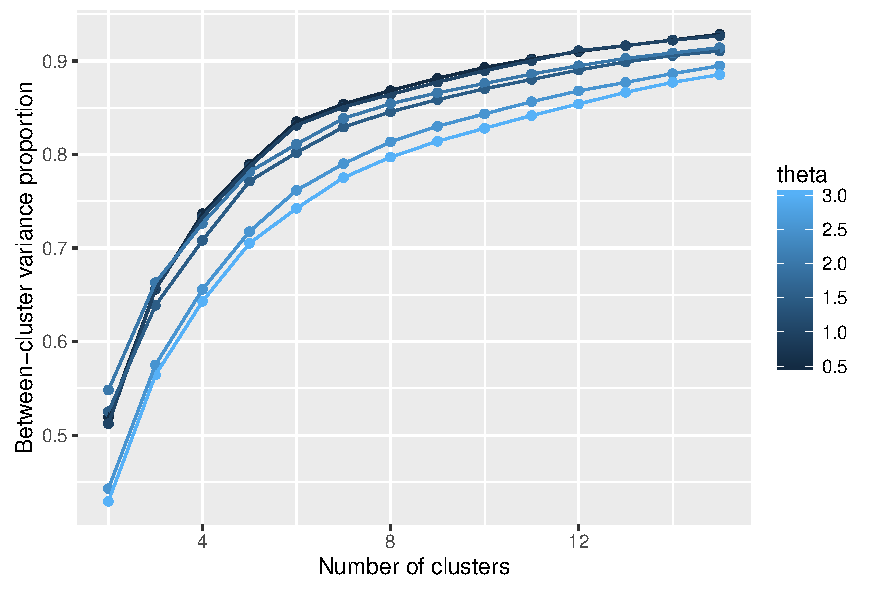
\includegraphics[width=0.49\linewidth]{Figures/CausalityRegimes/ccoef-knum_valuesFALSE_theta05-3.pdf}
%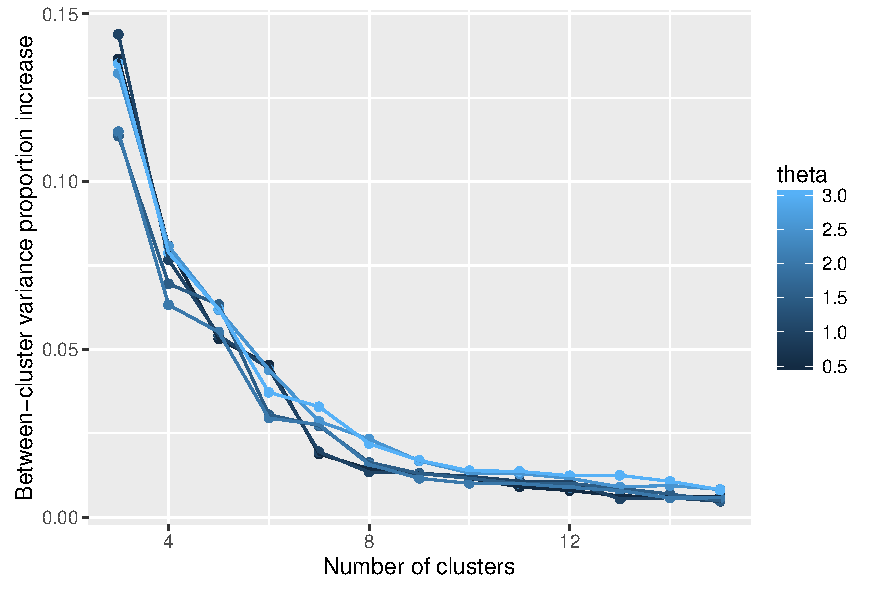
\includegraphics[width=0.49\linewidth]{Figures/CausalityRegimes/dccoef-knum_valuesFALSEtheta05-3.pdf}\\
%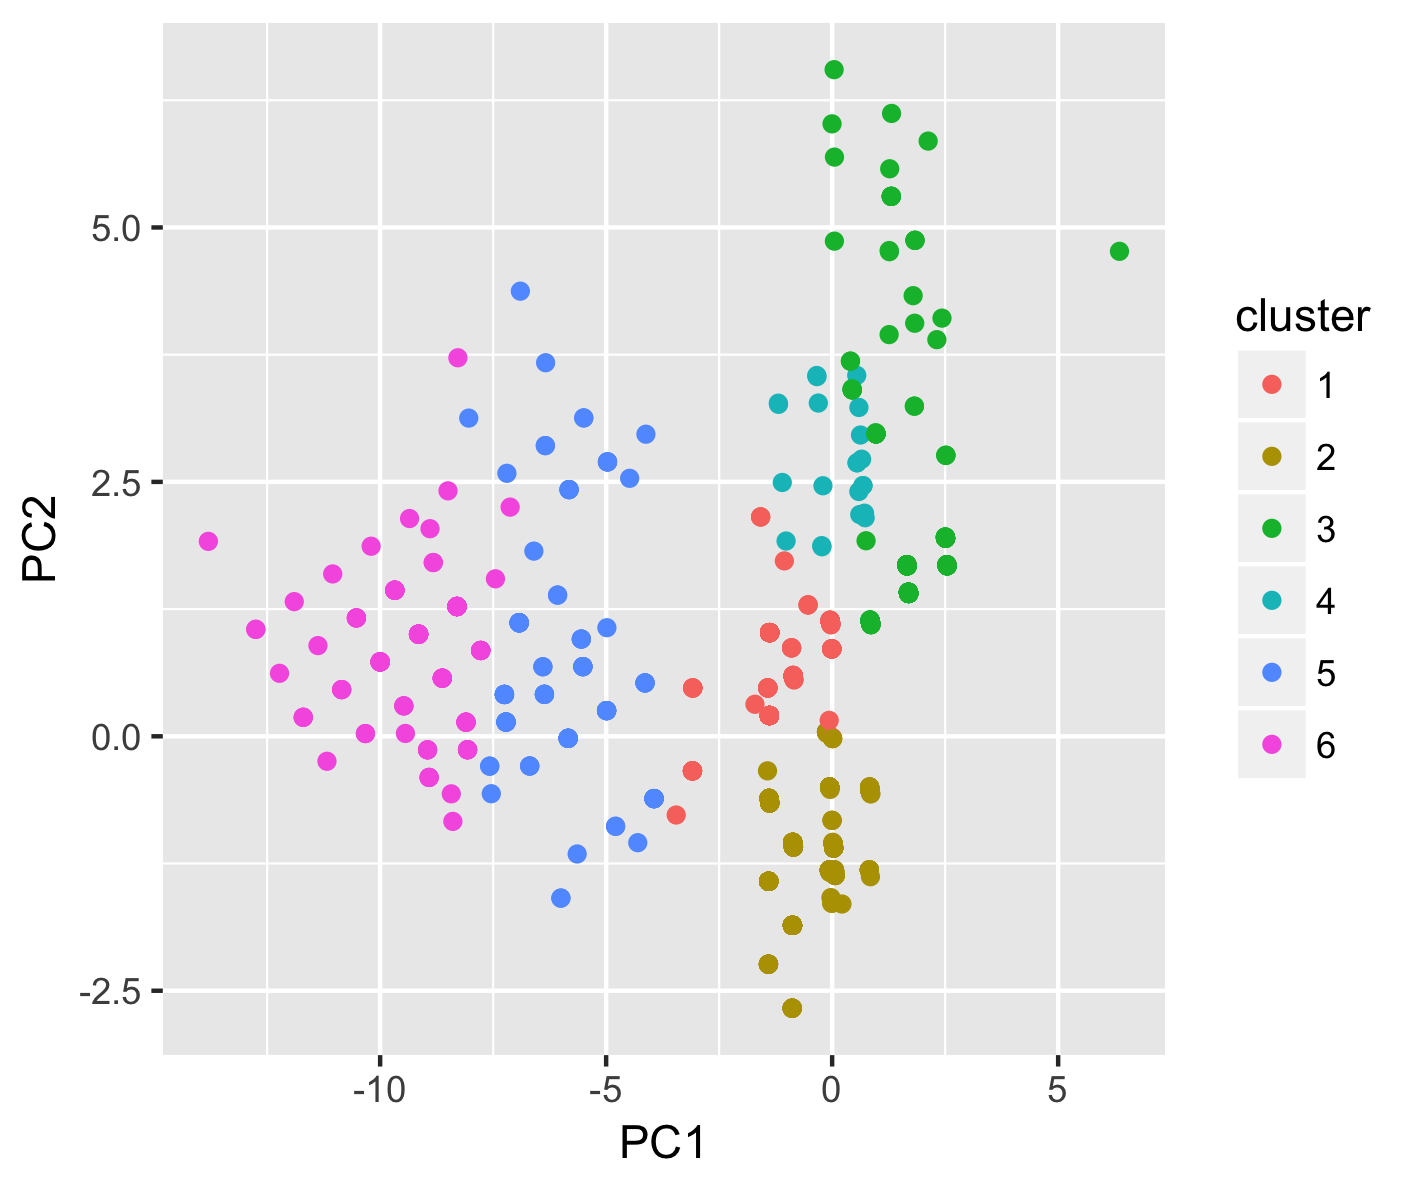
\includegraphics[width=0.4\linewidth]{Figures/CausalityRegimes/clusters-PCA-features_valuesFALSEtheta2_k6}
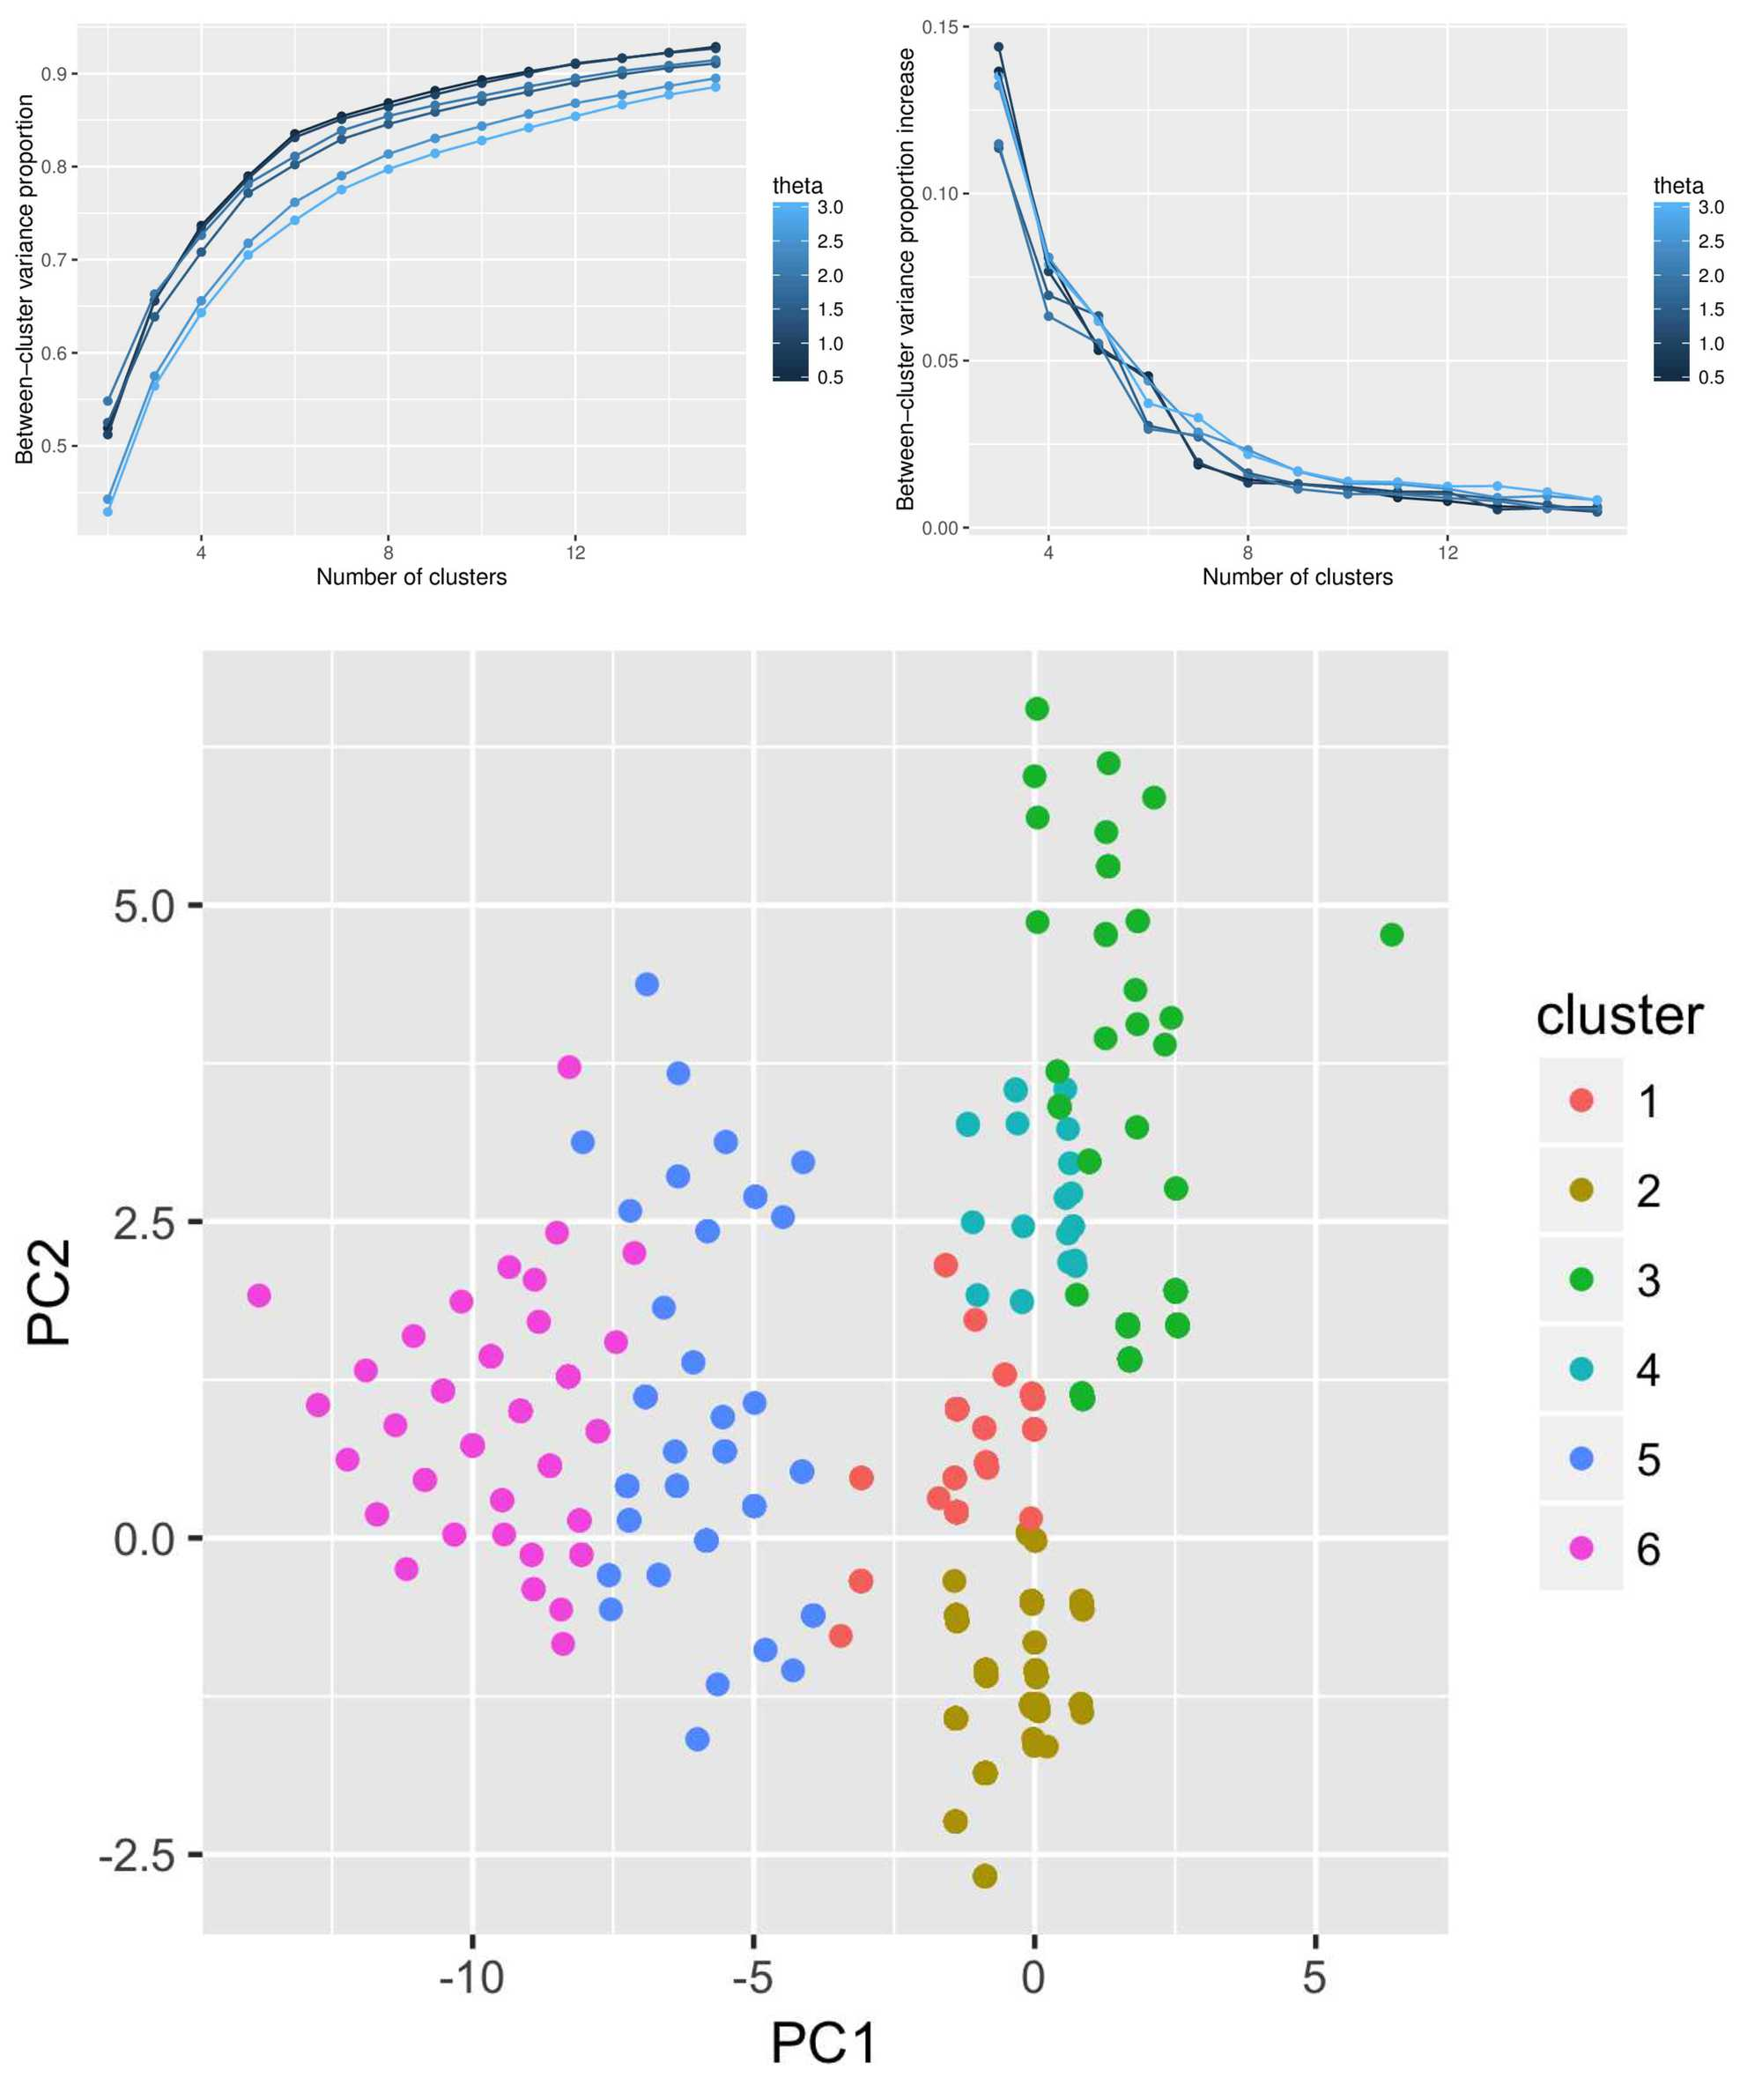
\includegraphics[width=\linewidth]{Figures/Final/A-causalityregimes-clustering.jpg}
\appcaption{\label{fig:app:causalityregimes:clustering}}{\textbf{Identification de régimes d'interactions endogènes par classification non-supervisée.} \textbf{(Haut Gauche)} Variance inter-cluster comme fonction du nombre de clusters. \textbf{(Haut Droite)} Dérivée de la variance inter-cluster. \textbf{(Bas)} \emph{Features} dans un plan principal (81\% de variance expliquée par les deux premières composantes).\label{fig:app:causalityregimes:clustering}}
\end{figure}
%%%%%%%%%%%%%%



\subsection{South Africa}{Afrique du Sud}


La Fig.~\ref{fig:app:causalityregimes:sudafcorrs} donne le comportement des corrélations estimées, en termes de corrélation absolue moyenne, et de proportion de corrélations significatives, en fonction de $d_0$ et de $T_W$. Elle donne également les profils de corrélations retardées pour les accessibilité pondérées, à l'origine et à la destination.


%%%%%%%%%%%%%%
\begin{figure}
%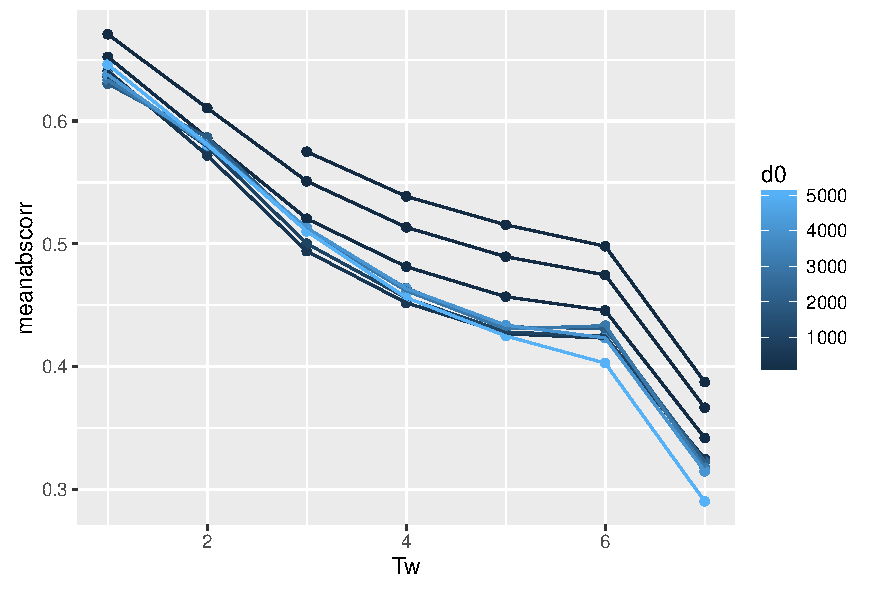
\includegraphics[width=0.49\linewidth]{Figures/CausalityRegimes/meanabscorrs}
%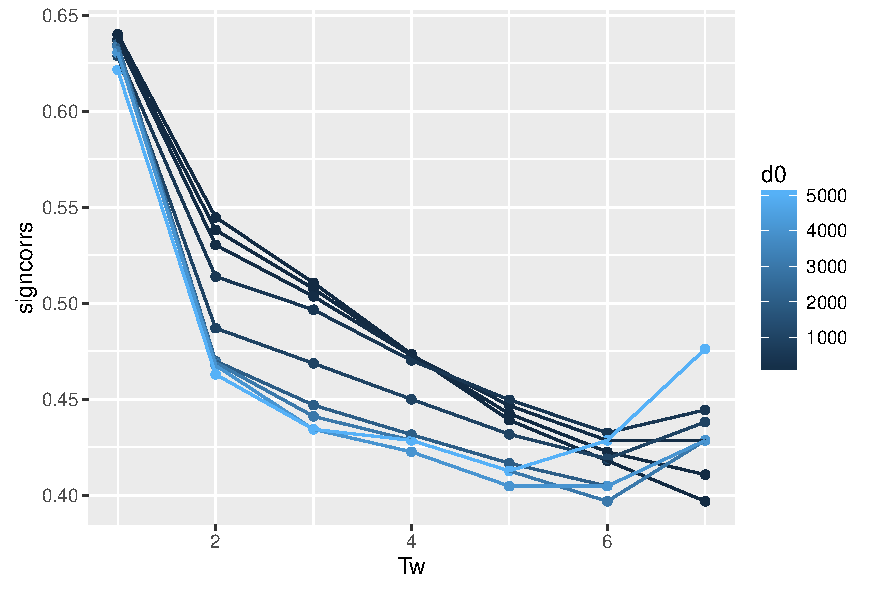
\includegraphics[width=0.49\linewidth]{Figures/CausalityRegimes/significantcorrs}\\
%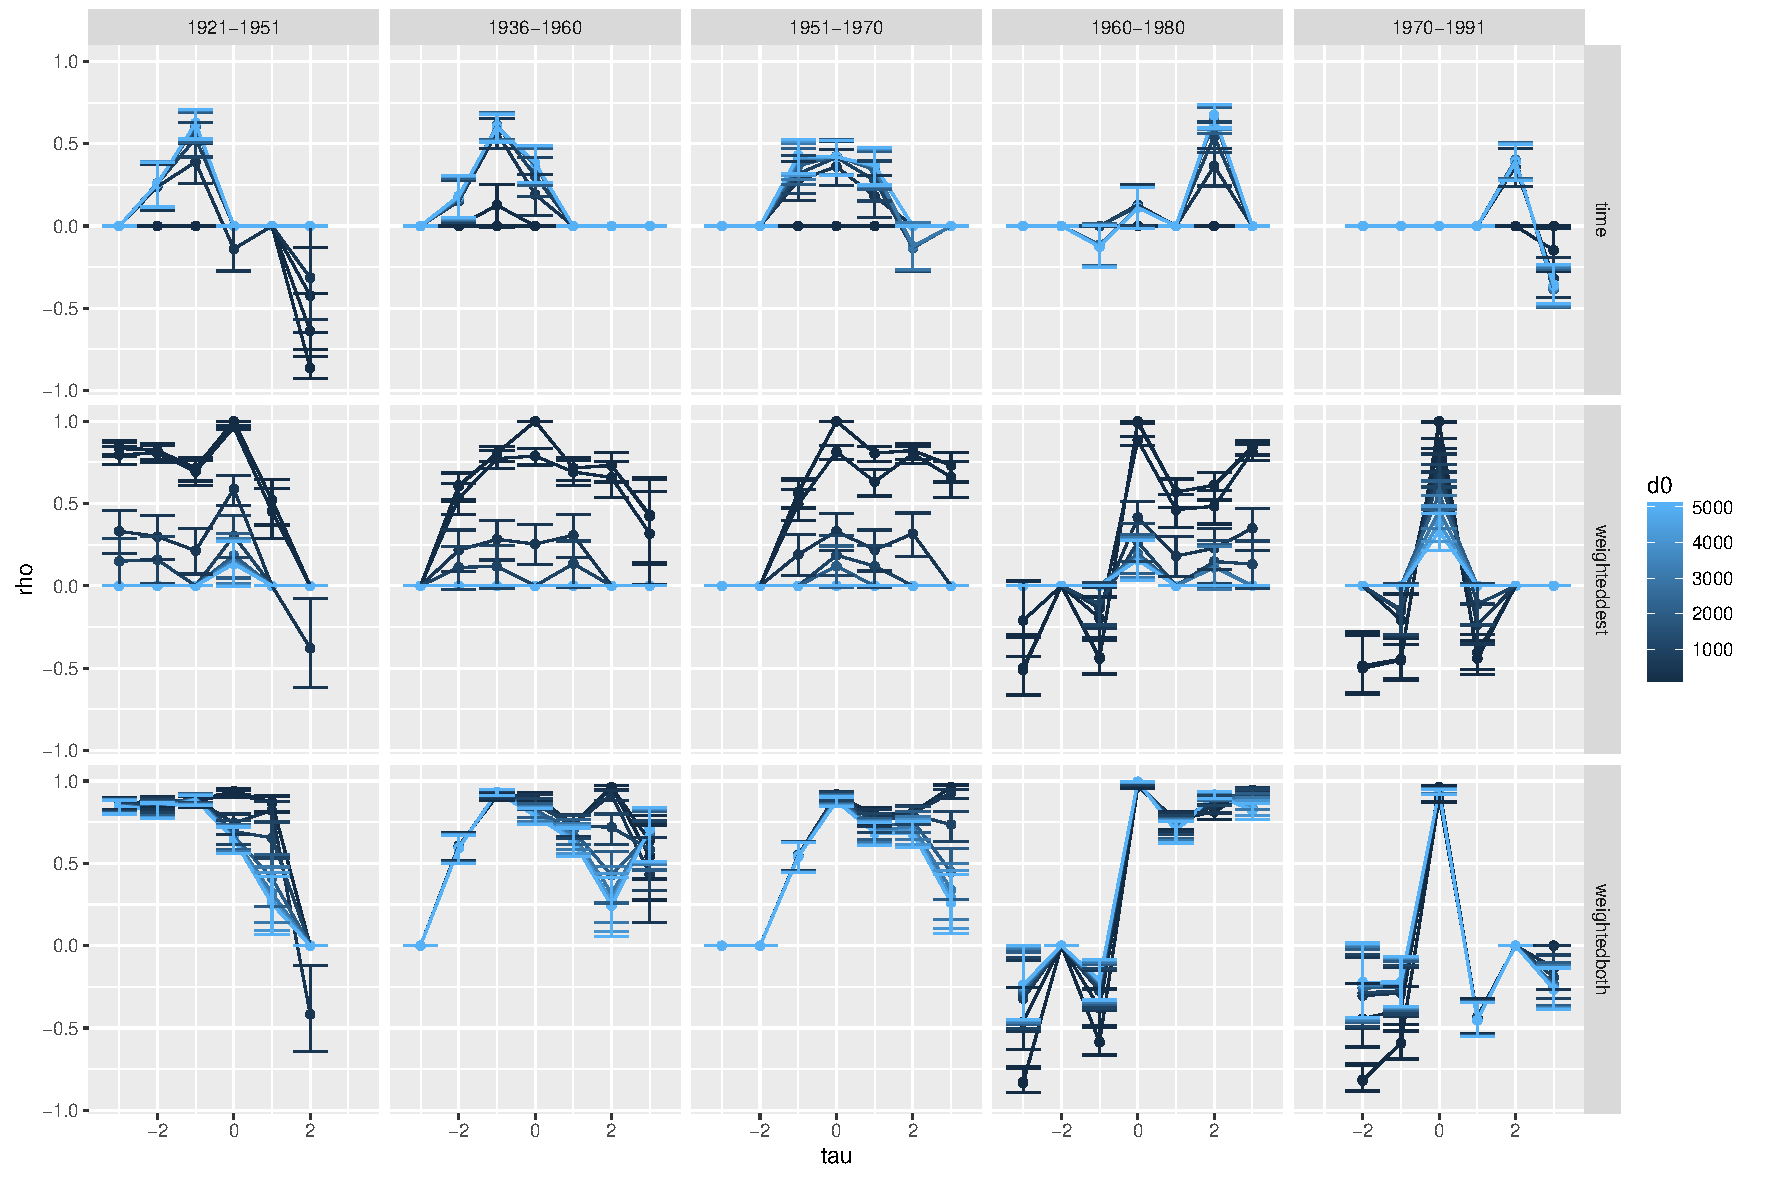
\includegraphics[width=\linewidth]{Figures/CausalityRegimes/laggedCorrs_Tw3}
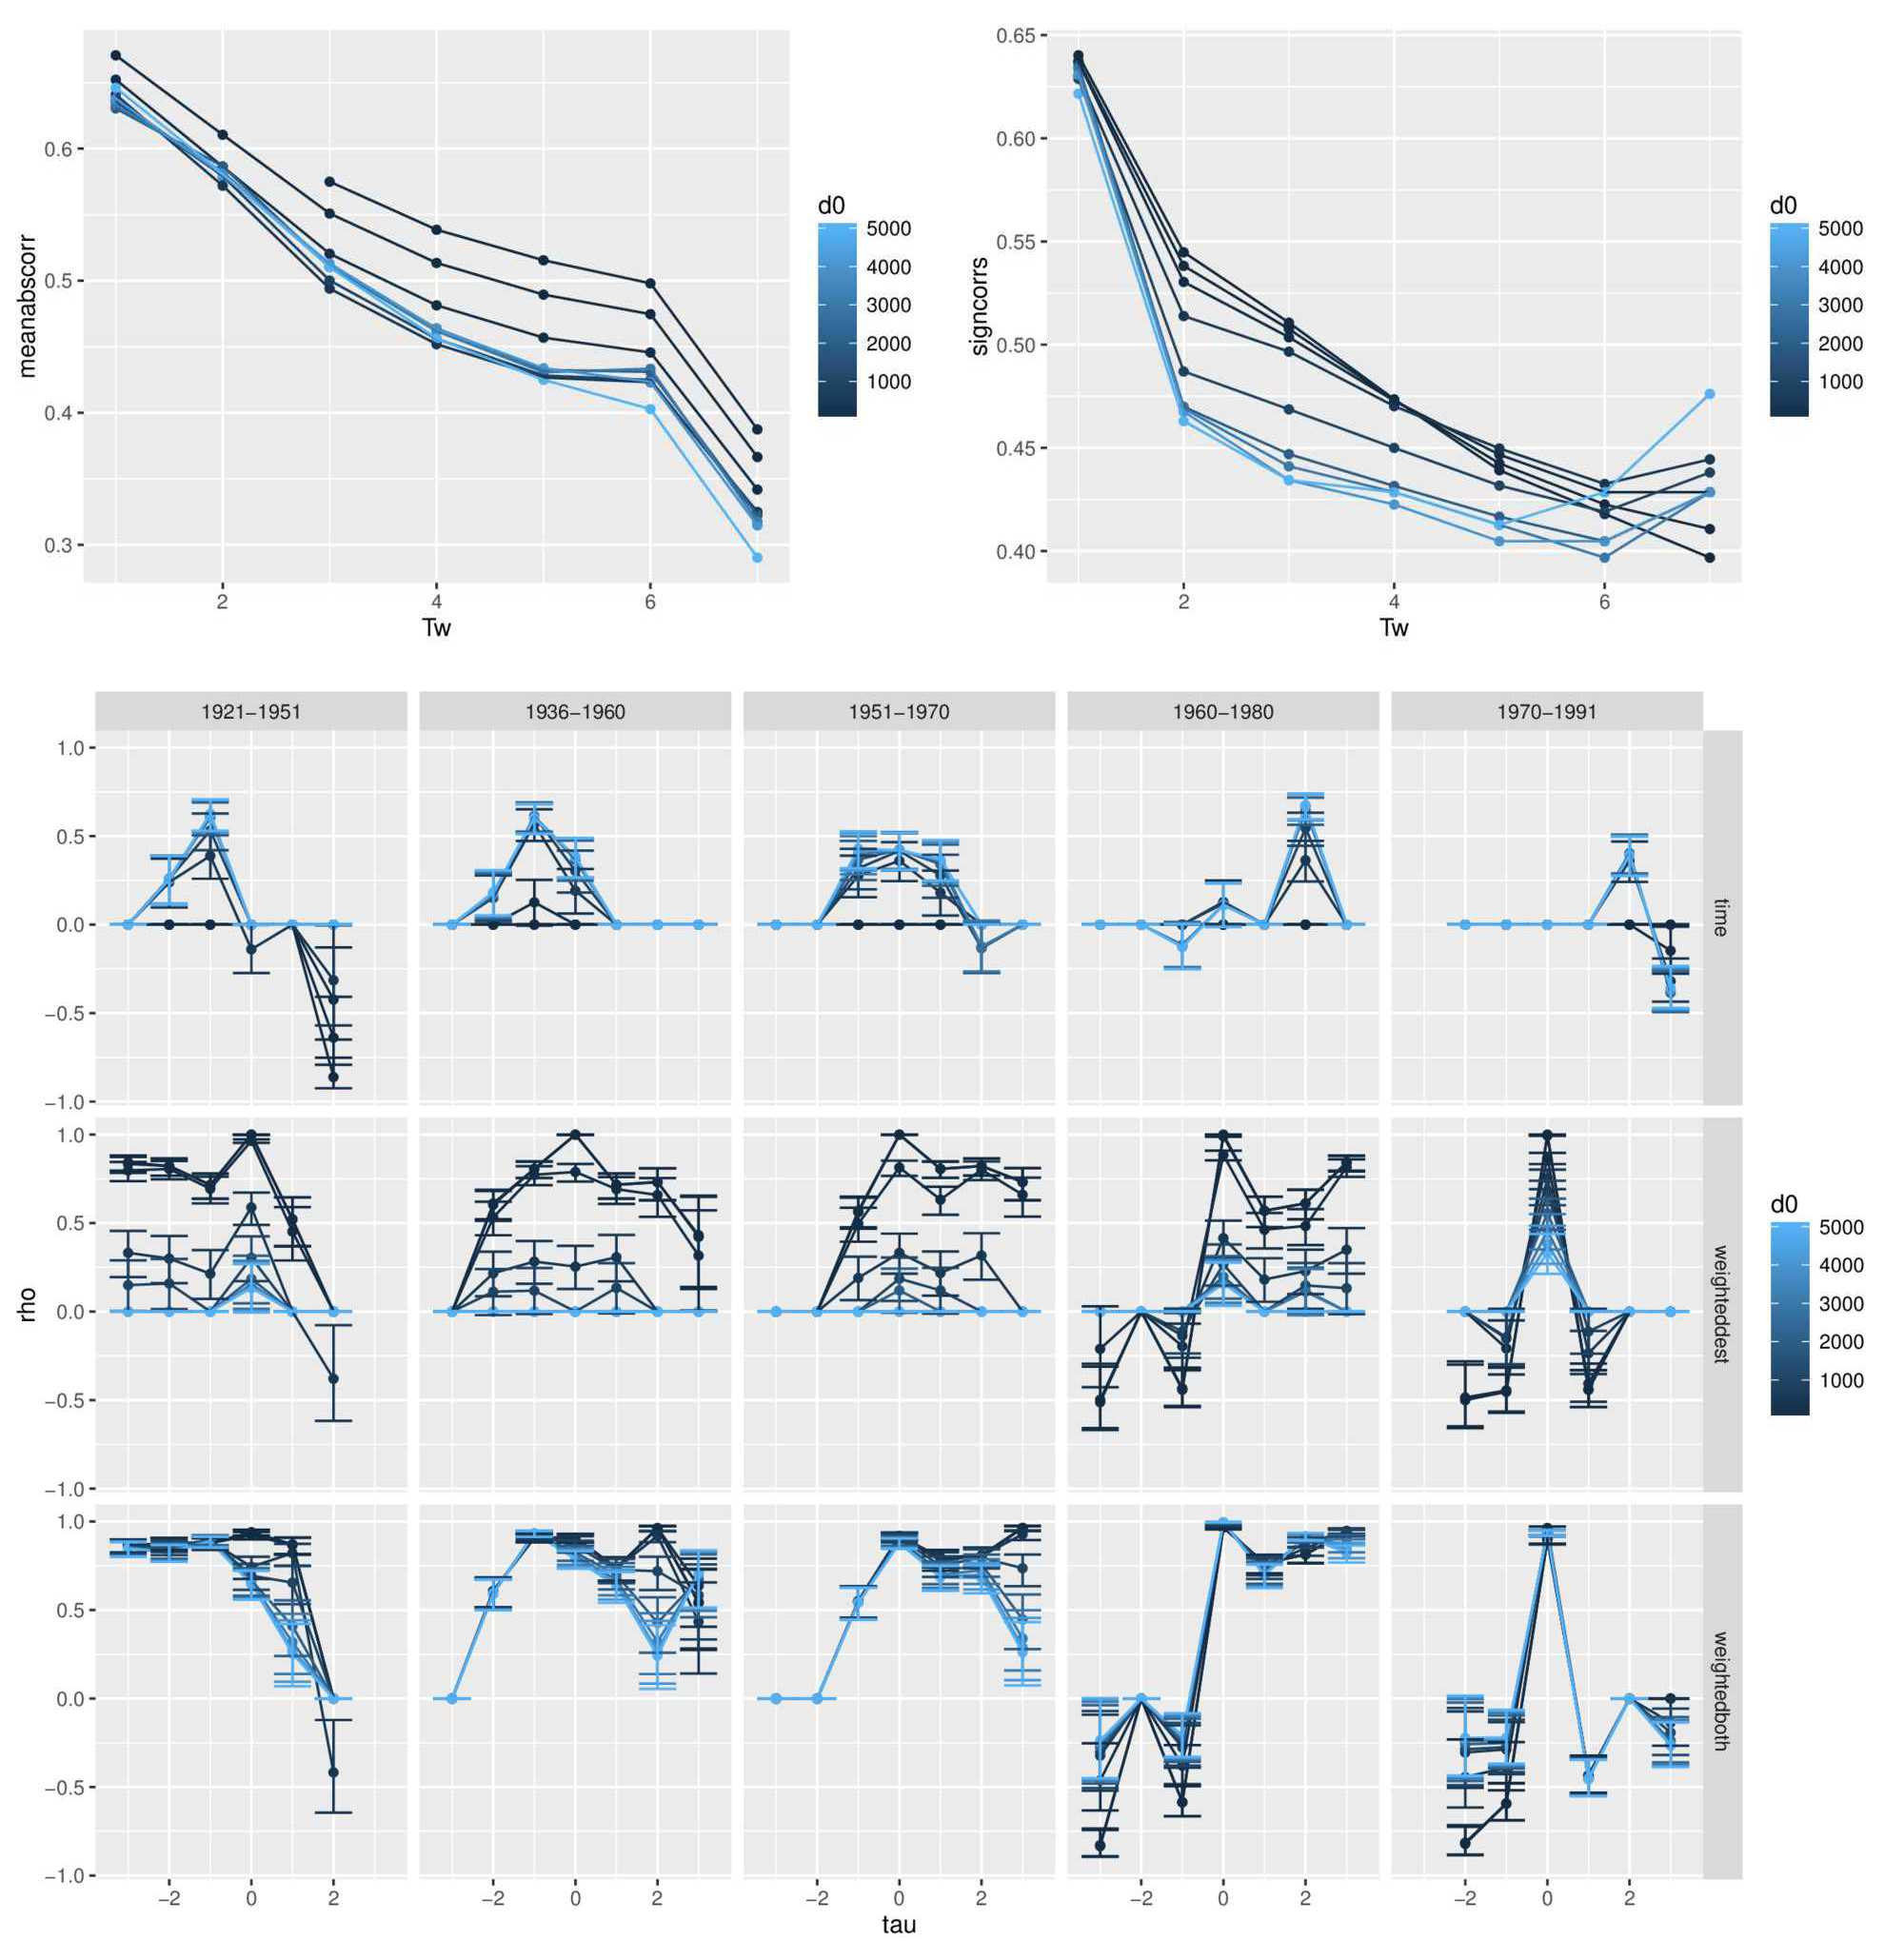
\includegraphics[width=\linewidth]{Figures/Final/A-causalityregimes-sudafcorrs.jpg}
\appcaption{\label{fig:app:causalityregimes:sudafcorrs}}{\textit{(Haut Gauche)} Corrélations absolues moyennes sur l'ensemble des retards, en fonction de la taille de la fenêtre temporelle $T_W$ (en nombre d'observations temporelles), pour différentes valeurs du paramètre de décroissance $d_0$ ; \textit{(Haut Droite)} Proportion de corrélations significatives, en fonction de $T_W$ pour $d_0$ variable ; \textit{(Bas)} Corrélations retardées en fonction du délai $\tau$, pour la taille optimale $T_W=3$, sur les différentes périodes successives (colonnes), pour les différents degrés de pondérations (première ligne $w_i=1$, deuxième ligne $w_i = 1,w_j=P_j/\sum_k P_k$, troisième ligne $w_i = P_i/\sum_k P_k,w_j=P_j/\sum_k P_k$), et pour $d_0$ variable (couleur).\label{fig:app:causalityregimes:sudafcorrs}}
\end{figure}
%%%%%%%%%%%%%%





\stars




%----------------------------------------------------------------------------------------


%\newpage

%%%%%%%%%%%%%%%%%%%%%%%
%\section{Spatio-temporal causalities}{Causalités spatio-temporelles}

%\label{app:sec:causalityregimes}




%%%%%%%%%%%%%%%
%\begin{figure}
%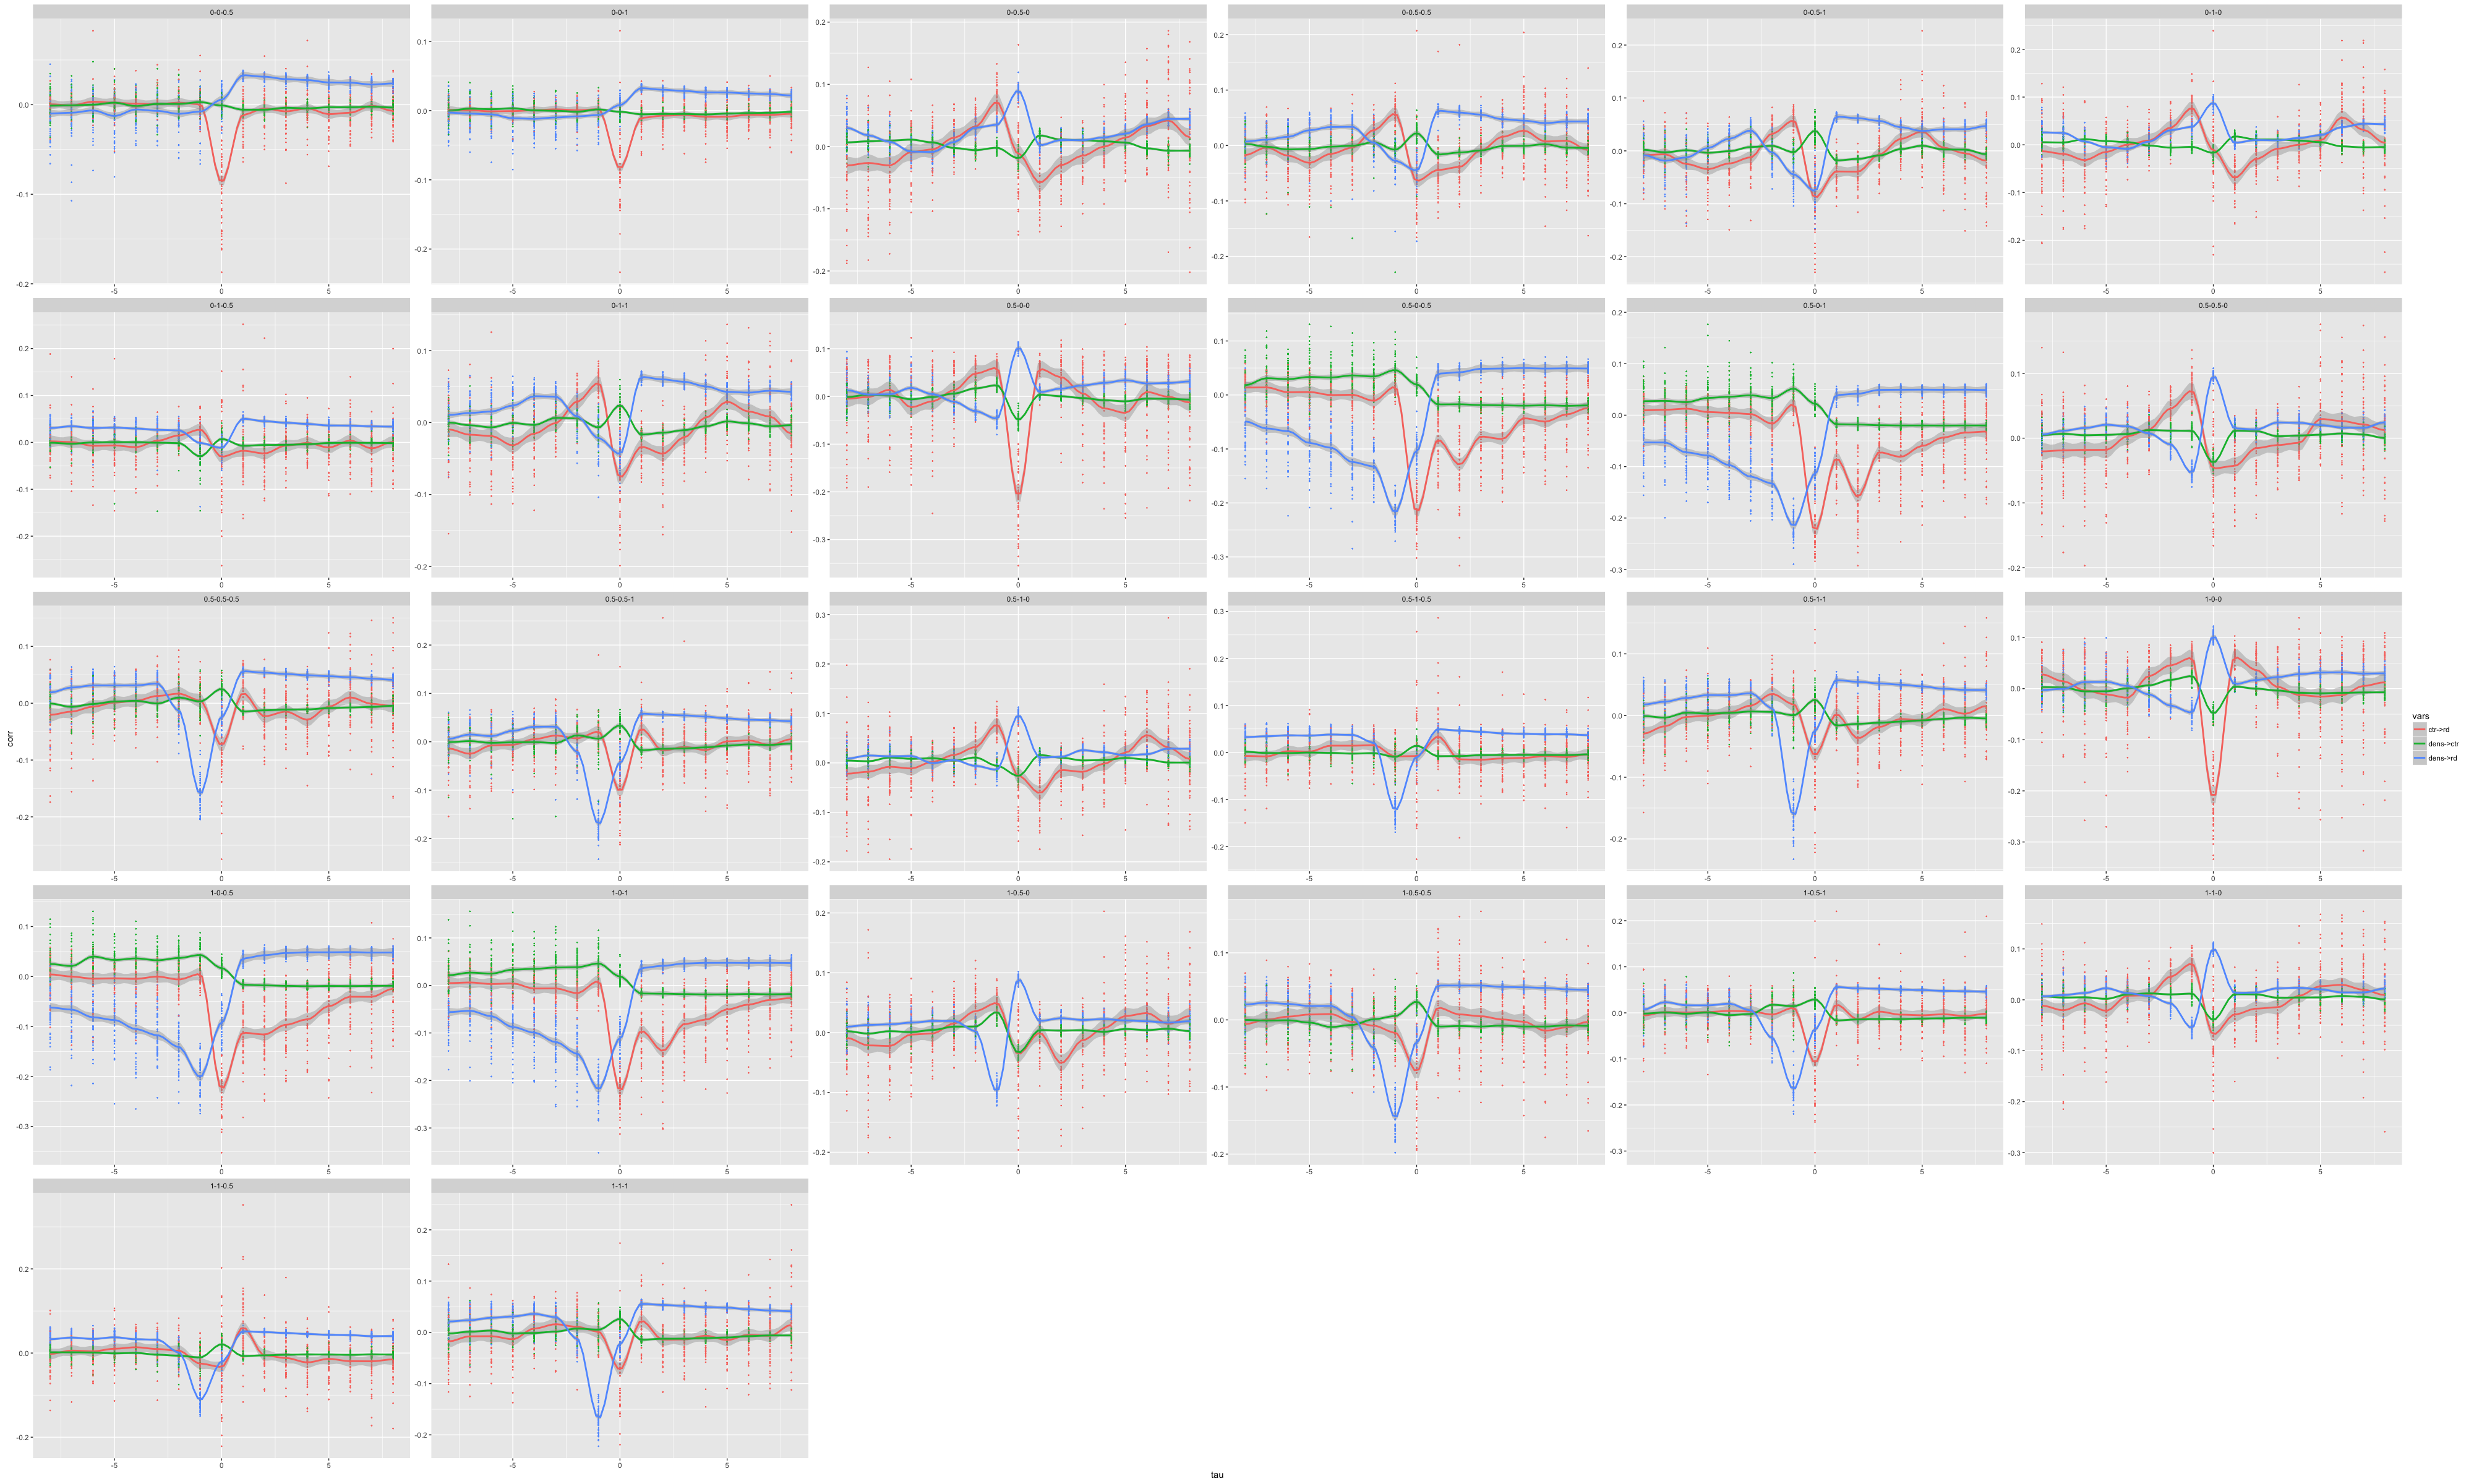
\includegraphics[height=\textwidth,angle=90]{Figures/SynthRBD/laggedcorrs_facet.png}
%\caption[][]{}{}
%\end{figure}
%%%%%%%%%%%%%%%



%----------------------------------------------------------------------------------------


\newpage

%%%%%%%%%%%%%%%%%%%%%%%
\section{Network Effects}{Effets de réseau}

\label{app:sec:interactiongibrat}








%We can develop the difference in information between two computational models, given by the difference of Kullback-Leibler information, 

%\[
%\Delta D_{KL} \left(M^{(1)}|M^{(2)}\right) = \Delta D_{KL} \left(S^{(1)}|S^{(2)}\right) + \left[ \Delta D_{KL} \left(S^{(2)}|M^{(1)}\right) + \Delta D_{KL} \left(S^{(1)}|M^{(2)}\right) \right]
%\]
 

%Under certain assumptions, the order of magnitude of second term appears to be negligible. More precisely, with $s^{(k)} = S^{(k)} - M^{(k)}$ and $f$ the probability density of reality the models try to approach, we have

%\[
%\begin{split}
%\Delta D_{KL} \left(S^{(k)}|M^{(k')}\right) & = \norm{\int f \cdot\log{\left(\frac{S^{(k)}}{M^{(k')}}\right)}} = \norm{\int f\cdot \log{\left(1 + \frac{s^{(k)}}{M^{(k')}}\right)}}\\
%& \simeq \norm{\int f \cdot \frac{s^{(k)}}{M^{(k')}}} \leq \frac{\sqrt{s_k}}{\norm{M^{(k')}}} \int f \leq 
%\end{split}
%\]
%



%%%%%%%%%%%%%%%%%%%%%%%%%%%
%\subsection*{Methodological implications}
%  - reflexions on iterative calibration, here ?
% no
%  - multimodeling ; back to the simple
% - bayesian iterative formulation ? (mcmc)
% - how does formulation influence ? equivalence in certain cases between stoch-cov and interdependent expectancies ? : under which conditions we can impose a covariance structure that produces interdependencies between expectancies ? seems to be a very broader question, need to do some thinking on that.











